% \begin{savequote}[75mm]
% Nulla facilisi. In vel sem. Morbi id urna in diam dignissim feugiat. Proin molestie tortor eu velit. Aliquam erat volutpat. Nullam ultrices, diam tempus vulputate egestas, eros pede varius leo.
% \qauthor{Quoteauthor Lastname}
% \end{savequote}

\chapter{Chapters}
\newpage

%%%%%%%%%%%%%%%%%
%%% PROTOCOLS %%%
%%%%%%%%%%%%%%%%%

\section[Integration of diverse bioactivity data into the Chemical Checker compound universe]{Chapter 3.1 -- Integration of diverse bioactivity data into the Chemical Checker compound universe}
\label{Chapter_3.1}
\setcounter{figure}{0}
\renewcommand{\thefigure}{3.\arabic{section}.\arabic{figure}}
% \hspace*{\fill} Work submitted to Nature Protocols (March 2024).
\hl{Work submitted to Nature Protocols (March 2024).}


% \addcontentsline{toc}{section}{Chapter 3.2 -- Protocols}
\subsection{Abstract}

Chemical signatures encode the physicochemical and structural properties of small molecules into numerical descriptors, forming the basis for chemical comparisons and search algorithms. The increasing availability of bioactivity data has improved compound representations to include biological effects, although bioactivity descriptors are often limited to a few well-documented molecules. However, unlike static chemical descriptors, these bioactivity signatures dynamically evolve with new data and processing strategies. Here, we present a python package aimed at modifying and generating novel bioactivity spaces and signatures, describing the main steps needed to leverage diverse bioactivity data with the current knowledge, as catalogued in the Chemical Checker (CC), using the predefined data curation pipeline. We illustrate the functioning of the protocol through four specific examples, including the incorporation of new compounds to an already existing bioactivity space, a change in the data pre-processing without altering the underlying experimental data, and the creation of two novel bioactivity spaces from scratch. Overall, this protocol offers a guideline for installing, testing and running the CC data integration approach on user-provided data, with the aim of extending the annotation presented for a limited number of small molecules to a larger chemical landscape.

\subsection{Introduction}

Small molecules are excellent tools for probing biological functions and continue to be the cornerstone of pharmaceutical companies. Synthetic chemical compounds present a complex structural code that, for the most part, has not been explored by the principles of natural evolution. Many pharmacological compounds are imperfect human inventions with sub-optimal bioactivities that lack a clear connection to their chemical structure. Often, the only way to approach the biological characterization of a compound is to assume it will have comparable bioactivities to compounds with similar chemical properties. The so-called ‘similarity principle’ has been the driving force of drug discovery efforts\cite{kumar_advances_2018}, and the measurement of compound similarities lays behind most of the approaches used to explore the vast drug-like chemical space (estimated in the range of 10\textsuperscript{33}-10\textsuperscript{66} molecules\cite{polishchuk_estimation_2013, bohacek_art_1996}). To assess such similarities, molecules are usually characterized using numerical fingerprints or descriptors\cite{cereto-massague_molecular_2015}, which encapsulate their main topological and physicochemical properties representing them in a format amenable for computational applications (e.g. QSAR\cite{yang_concepts_2022}).

In the last years, the extensive gathering and release of bioactivity data have shown that the similarity principle applies beyond standard chemical features, reaching to functional properties. For instance, small molecules that show similar sensitivity profiles across human tumor cell-lines or drugs that cause comparable side effects in patients tend to share mechanisms of action (MoA), even when they are structurally dissimilar\cite{holbeck_analysis_2010, seashore-ludlow_harnessing_2015, campillos_drug_2008}. Thus, bioactivity similarities offer an alternative means to functionally characterize small molecules, potentially providing insights closer to clinical observations and surpassing what is expected from merely inspecting chemical analogues\cite{petrone_rethinking_2012}.

%%%%%%%%%%%%%%%%
%%% FIGURE 1 %%%
%%%%%%%%%%%%%%%%


\begin{figure}[t!]
  \centering
  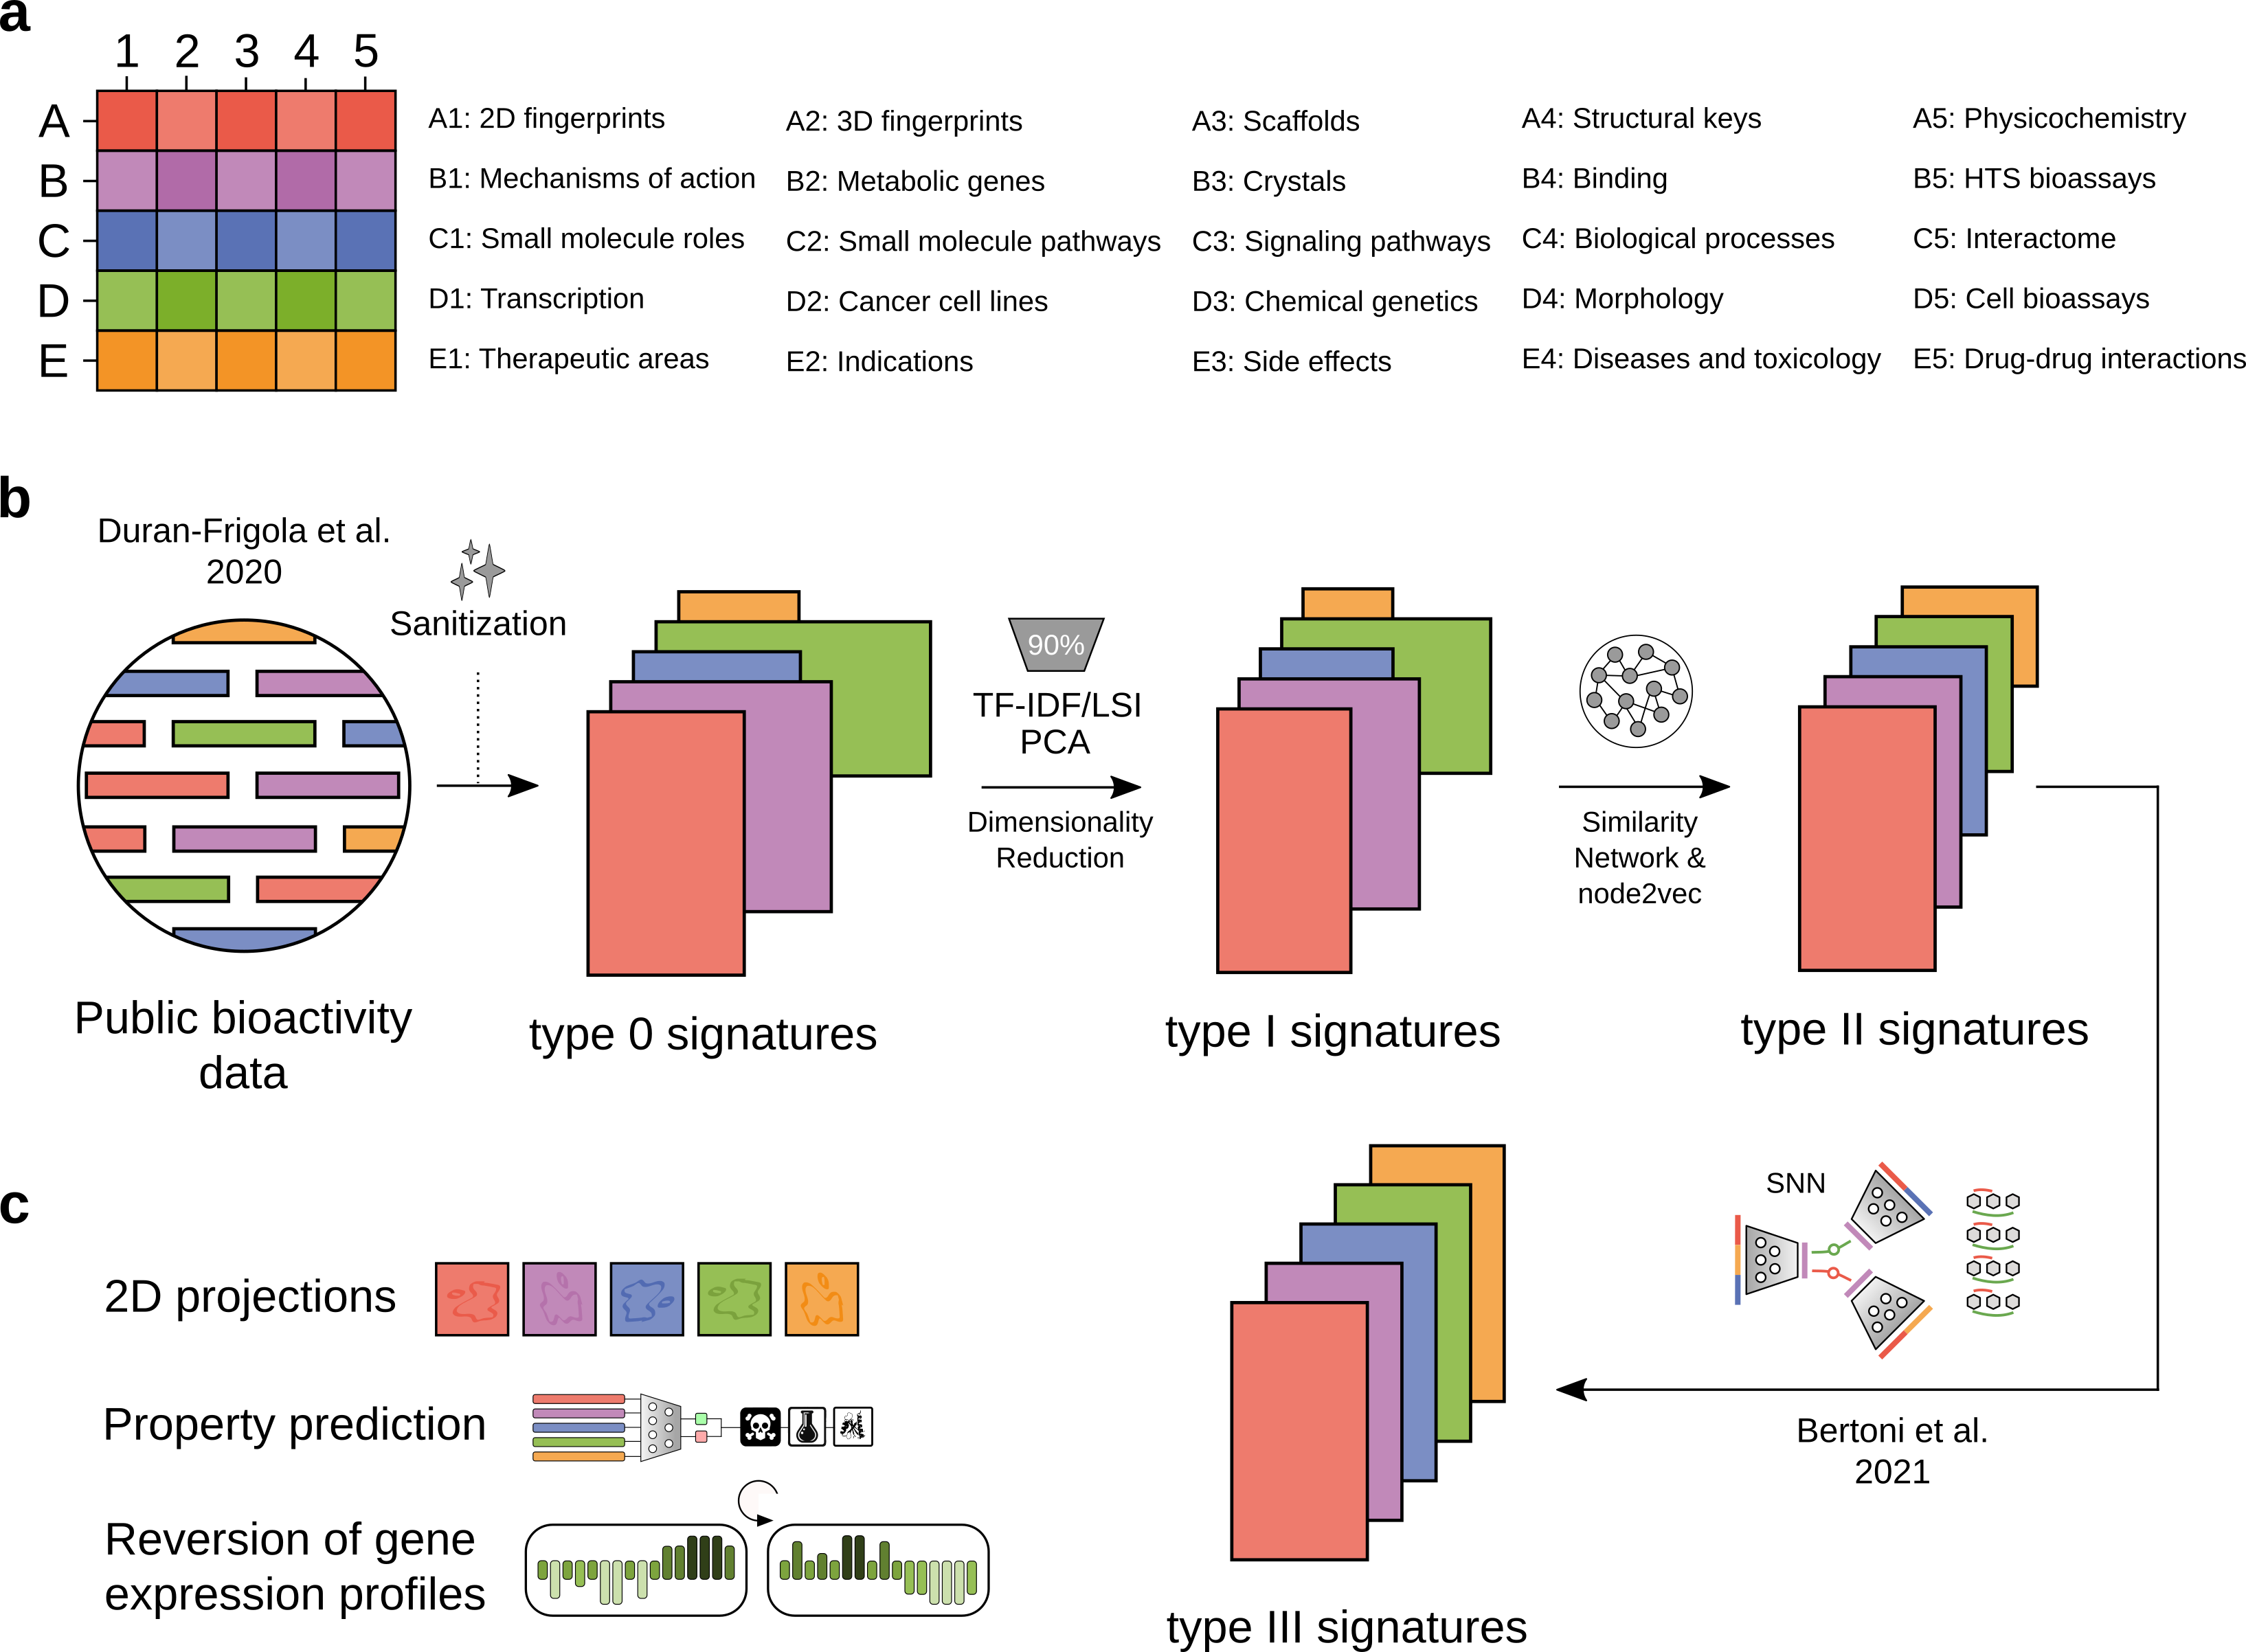
\includegraphics[width=\linewidth]{figures/Protocols/Main/CC.png}
  \caption{
    \textbf{CC Overview.} 
    \textbf{a)} Organization of the 25 CC spaces.
    \textbf{b)} Computational pipeline to build the CC and procedure to integrate bioactivity data in the CC universe. In brief, bioactivity data is sanitized (type 0 signatures), compressed (type I signatures), harmonized (type II signatures) and integrated with all the other data within the CC (type III signatures).
    \textbf{c)} Compound signatures are used in a variety of tasks, such as the characterization and visualization of large small molecule libraries, the prediction of multiple properties (e.g. toxicity, physicochemical properties, protein binding, etc.) and the reversion of gene expression profiles associated with specific disease states, among many others. 
    \rule[0ex]{\textwidth}{0.5pt}
  }
  \label{Protocols_Fig1}
\end{figure}



\phantomsection
\subsubsection{The Chemical Checker}

We recently developed the Chemical Checker (CC, Fig \ref{Protocols_Fig1}a), the largest collection to date of processed, harmonized and integrated bioactivity signatures for over 1 million compounds, whose biological effects had been experimentally determined\cite{duran-frigola_extending_2020}. Following the way in which we understand drug action, we organized data in 25 bioactivity spaces grouped in 5 levels of increasing biological complexity: from physicochemical and structural properties of small molecules (A) to the clinical effects they exert in human patients (E). In between, we collect the set of biological targets they bind (B), the perturbations they trigger in biological pathways (C) and the phenotypic effects they induce in cell-based assays (D). Unfortunately, bioactivity data become scarcer and more difficult to obtain as biological complexity increases (i.e. we have direct protein-binding data for \textasciitilde630k small molecules but only \textasciitilde6k compounds are annotated with clinical indications), meaning that bioactivity information remains limited for poorly characterized compounds. To address this problem, we developed a collection of deep neural networks to infer CC bioactivity signatures for any compound of interest\cite{bertoni_bioactivity_2021, comajuncosa-creus_stereochemically-aware_2024}, based on the observation that the different bioactivity spaces are not completely orthogonal, and thus similarities of a given bioactivity type (e.g. targets) can be transferred to other data kinds (e.g. therapeutic indications). Moreover, we showed that the inferred bioactivity signatures are useful to navigate the chemical space in a biologically relevant manner and improve the performance of biophysics and physiology activity prediction activities with respect to chemistry-only based classifiers. In general, we believe that bioactivity signatures associated to small molecules have the power to reintroduce the biological complexity at the early stages of the drug discovery process, overcoming some of the problems associated with target-based approaches. For instance, using CC signatures, we were able to identify three compounds able to revert transcriptional signatures related to Alzheimer’s disease \textit{in vitro} and \textit{in vivo}\cite{pauls_identification_2021}. Moreover, using CRISPR-Cas9 and shRNA perturbation experiments as templates, we also identified several small molecules that mimicked the phenotypic effects of biodrugs (e.g. daclizumab, ustekizumab, cetuximab, etc.), often through a different MoA that did not directly modulate the activity of their primary targets (e.g. IL-2R, IL-12 and EGFR)\cite{duran-frigola_extending_2020}, and targeted cancer proteins though to be undruggable\cite{bertoni_bioactivity_2021}.


The original 25 CC bioactivity spaces (Fig \ref{Protocols_Fig1}a) comprise data retrieved from publicly available databases at the time that were processed through a unified data curation and integration pipeline. Compound bioactivities are expressed in a vector-like format (i.e. signatures) and organized in increasing levels of abstraction: from raw data accounting for explicit knowledge (type 0 signatures) to inferred representations leveraging known bioactivity patterns (type III signatures). However, in the last years, new large-scale assays to capture biological responses to small molecule perturbations, and more efficient computational strategies to process them, are constantly appearing\cite{anglada-girotto_combining_2022, mitchell_proteome-wide_2023, offensperger_large-scale_2024}. Besides, there is an ever-growing number of laboratories and biotechnological companies that have their own in-house data and want to leverage it together with the bulk of known bioactivity information. Thus, in this manuscript, we present the complete computational protocol to generate novel bioactivity spaces and signatures, describing the main steps needed to leverage diverse bioactivity data with the Chemical Checker (type 0, type I, type II and type III signatures) using the predefined data curation and integration pipeline.

\phantomsection
\subsubsection{Overview of the Chemical Checker data integration pipeline}
\label{Overview of the Chemical Checker data integration pipeline}

The main input for the CC integration pipeline is a bioactivity data matrix encompassing compounds (rows, e.g. InChIKeys) and biological features (columns, unique strings: e.g. protein targets (B4), mechanisms of action (B1), clinical side effects (E3), etc.). Data might be categorical (e.g. binary), discrete or continuous.

\paragraph{-- Type 0 signatures --} \leavevmode

The very first step in the CC processing framework is to produce a sufficiently-curated and sanitized version of the raw bioactivity data (Fig \ref{Protocols_Fig1}b). To achieve this, features (columns) that are extremely sparse (i.e. occurring in few rows) or too prevalent (i.e. occurring in almost all rows) are removed from the matrix and those compounds (rows) showing no feature occurrences are discarded. In addition, not-available (NA) and infinite values are processed (median-imputed and max/min values, respectively) and low-Shannon entropy features are trimmed if the maximum number of allowed features is surpassed. Overall, type 0 signatures represent explicit knowledge, allowing direct interpretation while having variable dimensionality. 

\paragraph{-- Type I signatures --} \leavevmode

The second processing step implies a mild compression of type 0 signatures typically retaining 90\% of the original variance and thereby reducing the number of vector dimensions (Fig \ref{Protocols_Fig1}b). For discrete data, a term frequency–inverse document frequency (TF–IDF) transformation is used to weight features (columns) according to their information retrieval (i.e. more frequent features are less informative and thus become underweighted). After that, a Latent Semantic Indexing (LSI) dimensionality reduction technique is applied to the TF–IDF transformed data and LSI components explaining 90\% of the original variance are kept to build type I signatures. For continuous data, the matrix is first scaled column-wise (median 0, median absolute deviation 1 and capped at ±10) and then processed through a PCA. Analogously to discrete data, PCA components explaining 90\% of the original variance are kept to build type I signatures. Overall, type I signatures are better optimized for compound similarity calculations, although they no longer represent explicit knowledge and still have variable dimensionality.  

\paragraph{-- Type II signatures --} \leavevmode

The main purpose of type II signatures is to retain similarities at type I signature level while harmonizing the length of vectors among CC spaces (i.e. converting signatures of variable dimensionalities to 128-length vectors, Fig \ref{Protocols_Fig1}b). First, a similarity network is built considering nearest neighbors (NN) at type I signature level for each compound (small molecules represent the nodes in the graph and their similarities are the edges). Then, the node2vec algorithm is run to create an embedding for each molecule (node), encoding intrinsic relationships within the similarity graph. In this way and, although not directly interpretable, type II signatures capture explicit and implicit similarities in the data. Additionally, the fixed length (128) makes the concatenation of descriptors across bioactivity spaces cost-effective, while ensuring that each bioactivity space contributes equally to the overall representation.  


\paragraph{-- Type III signatures --} \leavevmode


The last step in the processing framework is the generation of type III signatures for the input compounds and for all the molecules in the CC, which capture and infer the similarity of the data at type I signature level (Fig 1b). The approach hinges on the insight that different CC spaces are not completely orthogonal and may show correlation to some extent. In short, for each CC space, a Siamese Neural Network (SNN) is trained over 10 million triplets of compounds (anchor, positive and negative molecules sampled at type I signature level) representing these input molecules by concatenating all available type II signatures. After being validated, the SNN generates novel signatures (type III) that retain the observed similarities at type I signature level and accounts for compound data present in every other bioactivity space of the CC, allowing the inference of a bioactivity signature even in the absence of data for the molecule of interest. It is worth mentioning that the generation of type III signatures is usually the most computationally expensive step in the CC data integration pipeline, and strongly benefits from parallelization (see \hyperref[Protocols_SupplementaryInformation]{Supplementary Information}).

Since most properties and similarities at type III signature level are inferred, each of them comes together with a measure of confidence called ‘applicability’ (from 0 to 1). Applicability scores evaluate the distance to training-set signatures, the robustness of the predicted signatures and the expectancy a priori given the known data. 

\paragraph{-- Additional remarks --} \leavevmode


The outlined pipeline includes numerous distinct steps, each possessing its own set of default options and parameters. For additional details on such parameters and further clarification of the mentioned steps we refer to the original publications\cite{duran-frigola_extending_2020, bertoni_bioactivity_2021} and our regularly maintained GitLab repository (\href{https://gitlabsbnb.irbbarcelona.org/packages}{https://gitlabsbnb.irbbarcelona.org/packages}). In addition, to monitor and evaluate data flow at each step of the CC integration pipeline, we have designed several analyses to assess the obtained results in a systematic manner. An exhaustive description of all benchmarking studies can be found in the \hyperref[Protocols_SupplementaryInformation]{Supplementary Information}. Finally, in order to generate CC type III signatures, the user needs to get all type II signatures from the current CC version. Signatures can be downloaded as plain data files from \href{https://chemicalchecker.com/downloads/root}{https://chemicalchecker.com/downloads/root}, or accessed through the CC REST API (\href{https://chemicalchecker.com/help}{https://chemicalchecker.com/help}, bottom of the page).


\phantomsection
\subsubsection{Building new Chemical Checker bioactivity spaces}
\label{Building_NEW_CC_BIOACTIVITY_SPACES}

To comprehensively illustrate the use of the protocol to build bioactivity spaces and signatures associated to small molecules, we adapt it to four distinct scenarios: i) introducing additional data into an existing CC bioactivity space (\textbf{B1.002} space), ii) creating a new version of an existing CC bioactivity space with a different strategy of input data processing (\textbf{D1.002} space), iii) creating a CC bioactivity space from a novel data type that fits the actual CC universe (i.e. human-derived data, \textbf{D6.001} space) and iv) creating a CC bioactivity space from a novel data type that does not fit the actual CC universe (i.e. measuring compound effects on bacterial species, \textbf{M1.001} space). The CC nomenclature to define the different bioactivity spaces first notes the space (i.e. A1-n, B1-n, etc) and then numbers the dataset or processing protocols used (i.e. 001, 002, etc).
\subsection{Results and discussion}


For each data integration task (4 in total) we first introduce the nature of the raw bioactivity data (Dataset description) and we then present and discuss the results obtained along the pipeline (Signaturization results). The implemented procedure is detailed in the \hyperref[Protocols_Methods]{Methods} section and illustrated in Fig \ref{Protocols_Fig2}.

%%%%%%%%%%%%%%%%
%%% FIGURE 2 %%%
%%%%%%%%%%%%%%%%


\begin{figure}[t!]
  \centering
  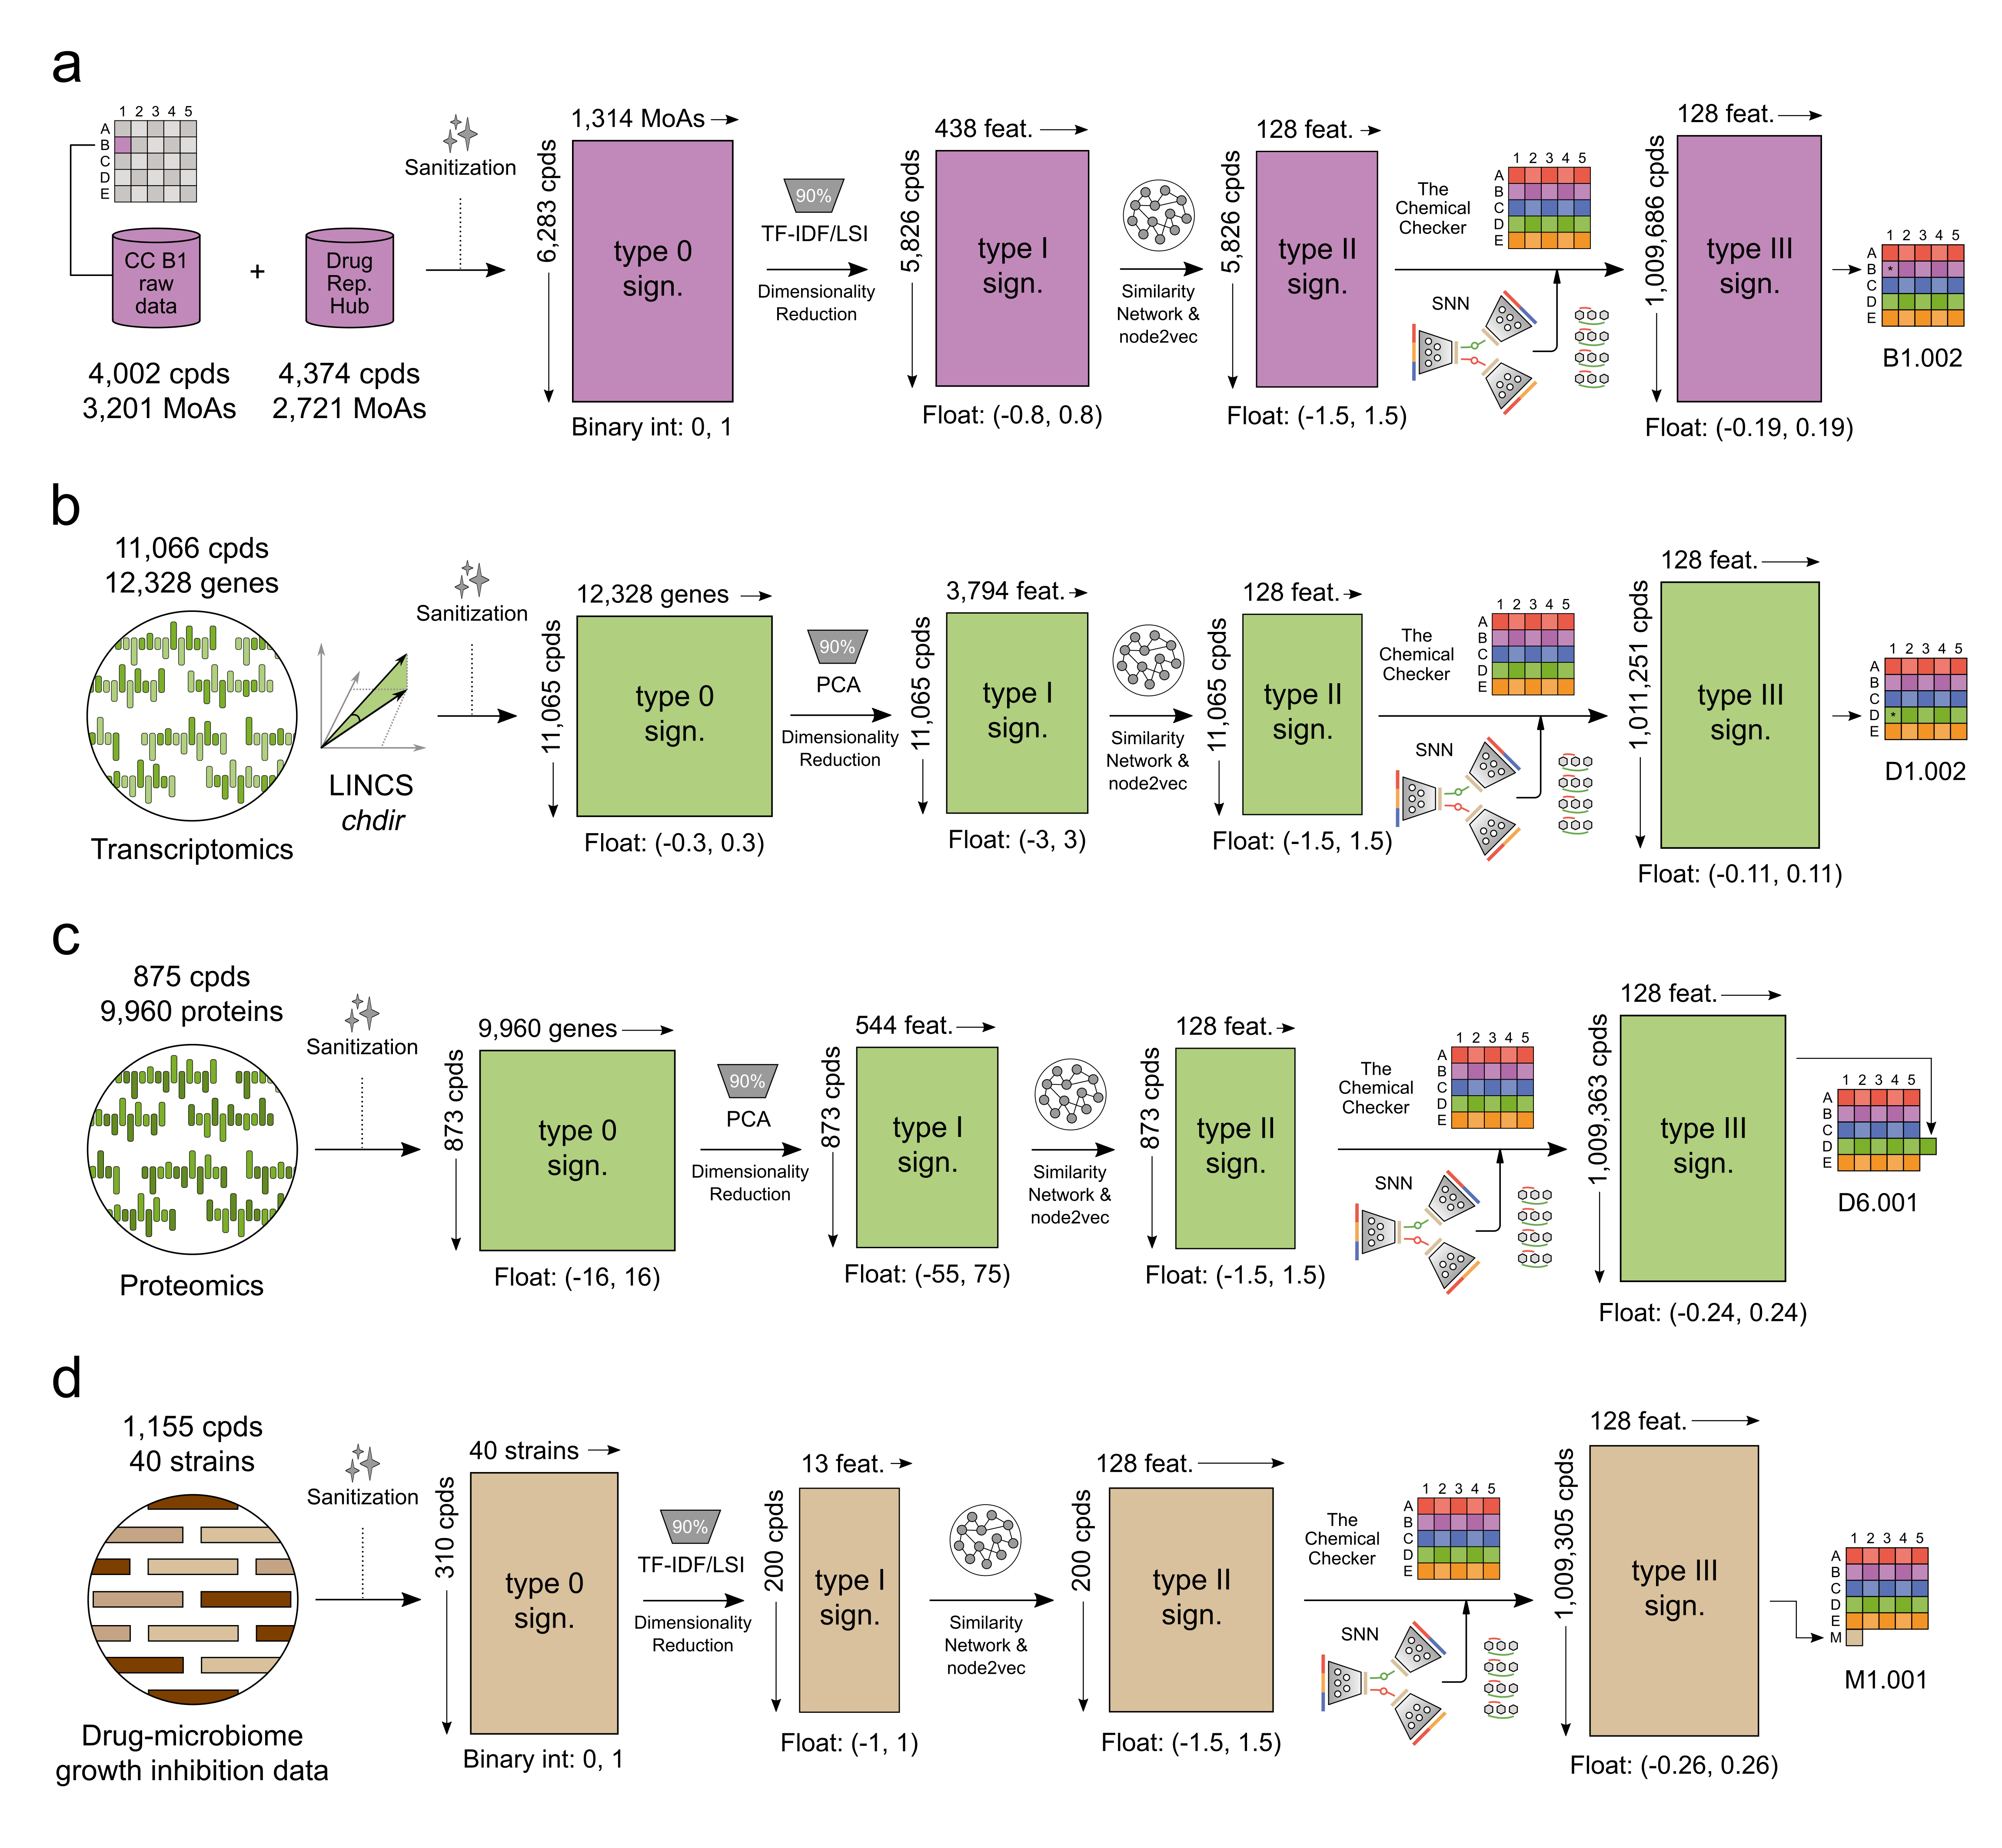
\includegraphics[width=\linewidth]{figures/Protocols/Main/Pipeline_v6.png}
  \caption{
    \textbf{CC Protocols case examples.} 
    \textbf{a)} Extending a preexisting CC space with additional bioactivity data (Task 1: B1.001).
    \textbf{b)} Rebuilding a preexisting CC space with a different strategy of processing the raw data (Task 2: D1.002).
    \textbf{c)} Create a new CC space from a novel data type that fits the current CC universe (i.e. human-derived data. Task 3: D6.001). 
    \textbf{d)} Create a new CC space from a novel data type that does not fit the current CC universe (i.e. measuring compound effects on bacterial species. Task 4: M1.001).
  }
  \rule[0ex]{\textwidth}{0.5pt}
  \vspace{-5mm}
  \label{Protocols_Fig2}
\end{figure}


%%%%%%%%%%%%%%%%%%%%%%%%%%%%
%%%%%%%%%%%%%%%%%%%%%%%%%%%%
%%%%%%%%  B1.002  %%%%%%%%%%
%%%%%%%%%%%%%%%%%%%%%%%%%%%%
%%%%%%%%%%%%%%%%%%%%%%%%%%%%


\phantomsection
\subsubsection{Task 1: Extending a preexisting CC space with additional bioactivity data (B1.002)}

\paragraph{-- Dataset description --} \leavevmode

The Drug Repurposing Hub\cite{corsello_drug_2017} is a centralized, comprehensive and curated collection of FDA-approved drugs, preclinical tool molecules, and clinically failed compounds for which safety has already been proven. All compounds are annotated with their chemical structures together with information about their mechanisms of actions (MoAs), approved disease indications and clinical trial status, if available.

The original CC B1 space (B1.001, MoA) was built using available data from ChEMBL (v.22) and DrugBank (v.4). The main purpose of this exercise is to extend the B1 space (namely B1.002) with the data from the Drug Repurposing Hub, accounting for 4,374 compounds and 2,721 mechanisms of action. 

\paragraph{-- Signaturization results -- \textasciitilde8 hours}  \leavevmode

First, we observed that the overlap between the original (ChEMBL and DrugBank) molecule-MoA pairs and those coming from the Drug Repurposing Hub was low, with only 3,342 out of the 11,971 new pairs already annotated in the original CC B1.001 space, which shows the value of incorporating this dataset. We merged all data (6,944 compounds and 4,626 mechanisms of action) and started the signaturization process. 3,312 seldom occurring MoAs and 661 compounds exhibiting null bioactivity profiles were filtered out in the first processing step (\textit{min\_feature\_abs} and \textit{min\_keys\_abs} parameters, respectively). Eventually, we obtained type 0 signatures for 6,283 compounds with 1,314 mechanisms of action. As illustrated in the diagnosis plots, the new B1.002 type 0 signatures were binary and highly redundant (Fig \ref{Protocols_FigS1}a). In the next step, we reduced data dimensionality and obtained type I signatures for 5,826 compounds, with 438 PCA components capturing 90\% of the variance. We then harmonized the number of features to match the CC data and generated type II signatures for these 5,826 molecules (128 features). Finally, we integrated the new B1.002 space together with the rest of the CC spaces and generated type III signatures for all 1,009,686 compounds (5,826 and 1,009,293 in B1.002 and the CC universe, respectively, with an overlap of 5,433 compounds). 

An important consideration is that similarities at the raw data level (type 0 signatures) may be partially diluted along the data contextualization pipeline (e.g. at type III signature level), when the data is eventually compressed and integrated with all the bioactivity data already contained in the CC. To further illustrate which spaces may be more affected in this regard, we have designed an evaluation process in which, for each new CC space and signature type, we assess the ability to recapitulate NN from a signature type at a lower level (Fig \ref{Protocols_Fig3}a). First, for the newly created B1.002 space, we defined a cutoff cosine distance for all signature types (0, 1, 2 and 3, i.e. 0, I, II and III) at a pvalue of 0.01 (10,000 randomly selected compounds x 10 subsamples, considering the average value). Then, for each combination of signA-signB, we evaluated the ability of signB to recapitulate NN defined at signA level with a pvalue of 0.01 (for each combination, 2,500 random molecules, 5 subsamples; totaling 6 combinations of signature type pairs). In the case of the B1.002 space, we observed that type III signatures were able to greatly recapitulate similarities observed at the raw bioactivity data level (type 0 signatures, AUROCs\textasciitilde0.85, Fig \ref{Protocols_Fig3}b). In addition, we also observed that applicability values associated with type III signatures were fairly in line with the values obtained for the original CC bioactivity spaces (Fig \ref{Protocols_Fig3}c).

Interestingly, we observed that, apart from including a higher number of compounds and MoAs, the new B1.002 space was less redundant than B1.001 (Fig \ref{Protocols_FigS1}, Fig \ref{Protocols_FigS2} and our \href{https://gitlabsbnb.irbbarcelona.org/packages/protocols}{Gitlab repository}). A tSNE 2D representation of these two spaces show how the incorporation of new data populates some areas of the target space not previously covered, and that the new B1.002 space was able to better recapitulate known MoAs and ATCs for annotated compounds (Fig \ref{Protocols_FigS3}). 

A global picture of the pipeline with detailed steps, numbers and timings is shown in Fig \ref{Protocols_Fig2}a. Diagnosis plots for all signatures are shown in Fig \ref{Protocols_FigS1} and Fig \ref{Protocols_FigS2}. B1.002 type 0, I, II and III signatures are available in \hyperlink{https://zenodo.org/records/14000467}{https://zenodo.org/records/14000467}. 

\begin{Figure_modified}
  \centering
  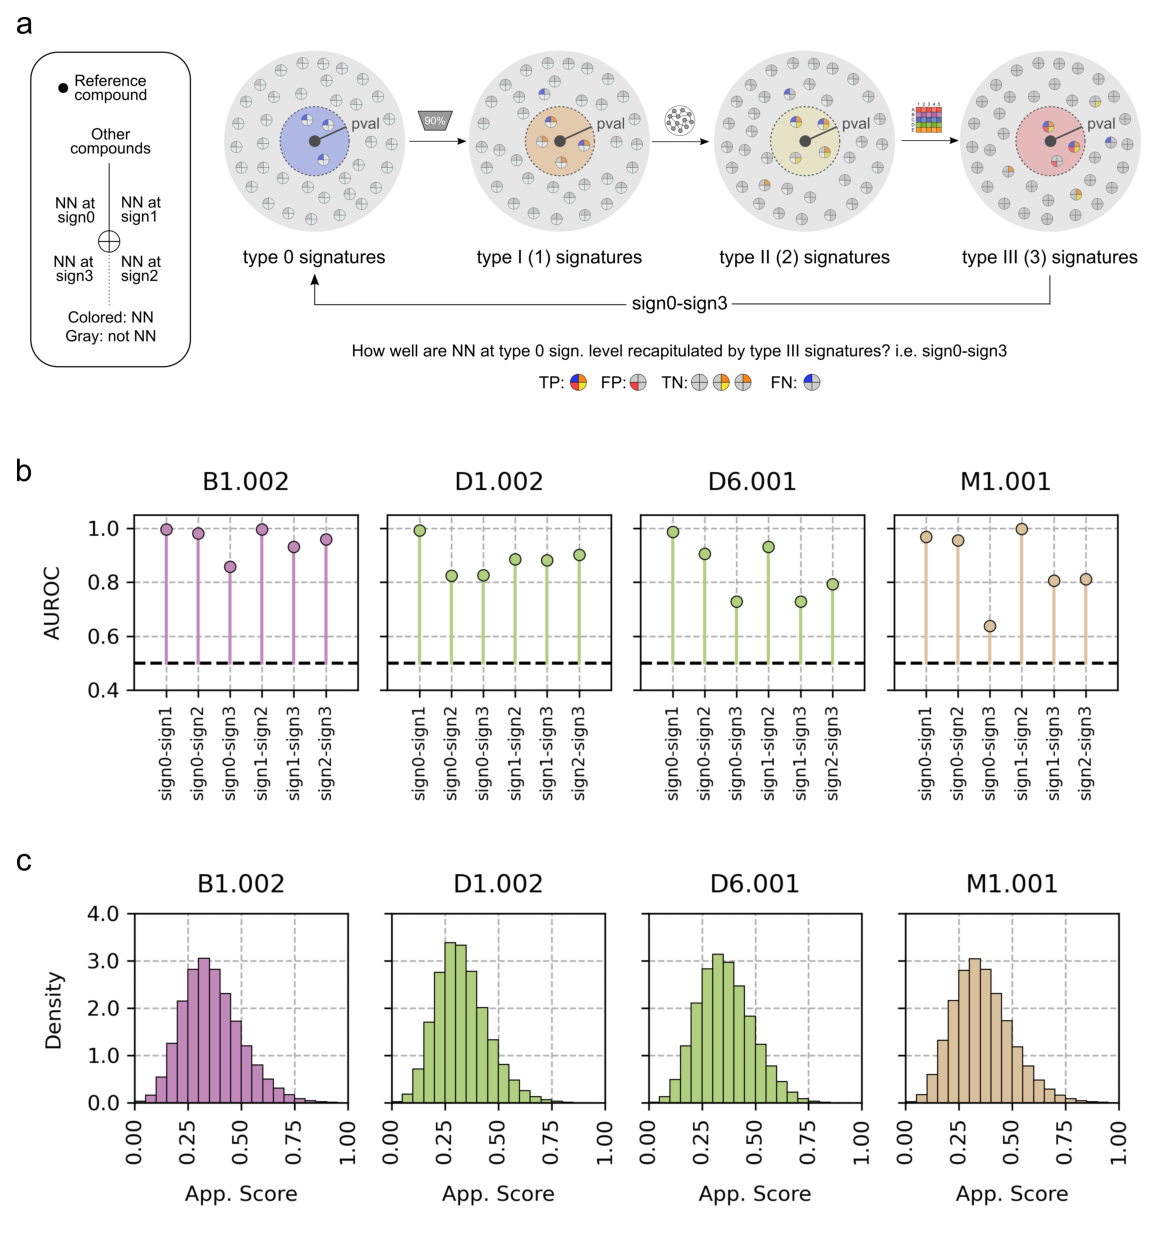
\includegraphics[width=\linewidth]{figures/Protocols/Main/Fig3.eps}
  \caption{
    \textbf{Quantitative evaluation of the signaturization process.} 
    \textbf{a)} Graphical representation of the validation strategy (from left to right). A reference compound (black circle) has a set of NN defined at type 0 signature level. Those NN may or may not be NN along the data compression, harmonization and integration pipeline. The better the ability to recapitulate NN defined at type 0 signature level by any other signature type, the fewer amount of information is lost along the computational pipeline. 
    \textbf{b)} For each newly created CC space and pair of signature types (signA-signB), ability (y-axis, AUROC) from signBs to recapitulate NN defined at signA level. In brief, we defined a cutoff cosine distance for all signature types (0, I, II and III) at a pvalue of 0.01 (10,000 randomly selected compounds x 10 subsamples, considering the average value). Then, for each combination of signA-signB, we evaluated the ability of signB to recapitulate NN defined at signA level with a pvalue of 0.01 (for each combination, 2,500 random molecules, 5 subsamples; totalling 6 combinations of signature type pairs). 
    \textbf{c)} For each newly created CC space, distribution of applicability values associated to the generated type III signatures.
  }
  \vspace{-5mm}
  \rule[0ex]{\textwidth}{0.5pt}
  \vspace{-9mm}
  \label{Protocols_Fig3}
\end{Figure_modified}

%%%%%%%%%%%%%%%%%%%%%%%%%%%%
%%%%%%%%%%%%%%%%%%%%%%%%%%%%
%%%%%%%%  D1.002  %%%%%%%%%%
%%%%%%%%%%%%%%%%%%%%%%%%%%%%
%%%%%%%%%%%%%%%%%%%%%%%%%%%%



\phantomsection
\subsubsection{Task 2: Rebuilding a preexisting CC space with a different strategy of processing the raw data (D1.002)}


\paragraph{-- Dataset description --} \leavevmode

Gene expression (GEx) responses after compound perturbation provide a convenient way to connect diseases to drugs. Since the release of the Connectivity Map (CMap) and LINCS resources, compound GEx signatures have allowed the identification of potential treatments for diverse diseases \cite{pauls_identification_2021, sawada_predicting_2018, chen_reversal_2017} and have provided new insights on compounds’ mechanisms of action (MoAs), compounds’ target and sensitivity responses. Given the significant value of these screenings, conscious efforts have been carried out to remove potential sources of noise and inherent biases, unearthing higher and more robust biological signals. Particularly relevant has been the implementation of the Characteristic Direction (chdir) method\cite{clark_characteristic_2014} which, having been tailored in the context of compound perturbation responses, it is not only more suitable for detecting meaningful GEx changes but also provides a means to identify non-robust, noisy profiles. Thus, we re-processed raw LINCS data using the chdir GEx profile protocol, as indicated by the authors. Eventually, we ended up with 11,066 compounds (rows) and 12,328 genes (columns), which significantly enhanced the interpretability compared to the previous processing method. In the next paragraphs we exemplify the rebuilding of the D1 space with this new pre-processing protocol (D1.002). 

\paragraph{-- Signaturization results -- \textasciitilde9 hours}  \leavevmode

After processing the data, we started the rebuilding of the D1 space (D1.002) with 11,066 compounds (rows) and 12,328 genes (columns), while our old processing (D1.001) contained 14,098 compounds and 7,967 CMap features. This reduction in the number of compounds is due to the additional chdir filtering step that accounts for the robustness in the GEx replicates. Now, each compound-gene pair was associated with a numerical value representing the induced gene expression change. After creating the new CC instance and loading the preprocessed bioactivity data, we obtained type 0 signatures for 11,066 compounds against 12,328 genes. It is important to note that, in the generation of type 0 signatures, we set the number of maximally considered features in the sanitization process up to 13k, since the default value is 10k. In addition, we observed that signatures were not redundant and that most values were in the [-0.05, 0.05] range (Fig \ref{Protocols_FigS4}a). Then, we obtained type I signatures for 11,065 compounds with 3,794 dimensions and generated harmonized type II signatures for these 11,065 compounds (Fig \ref{Protocols_FigS4}b, c). Finally, we integrated the D1.002 space with the rest of CC spaces and obtained type III signatures for all 1,009,305 compounds (Fig \ref{Protocols_FigS5}). To assess the capacity of type I, II and III signatures to recapitulate NNs defined at type 0 signature level (raw bioactivity data), we implemented the methodology extensively described in the previous section and illustrated in Fig \ref{Protocols_Fig3}a. In this task, we also observed that type III signatures were able to greatly recapitulate similarities defined at the raw bioactivity data level (type 0 signatures, AUROCs\textasciitilde0.83, Fig \ref{Protocols_Fig3}b) and showed applicability values in the same range of preexisting CC bioactivity spaces (Fig \ref{Protocols_Fig3}c).

A downstream comparison with the space obtained from our old processing (D1.001) confirmed the overall improved consistency of this new space, as illustrated by the better recapitulation of known drug bioactivity associations, including their MoA and therapeutic (ATC) areas (Fig \ref{Protocols_FigS6}). This exercise highlights the importance not only of the quality of the raw data employed to develop the bioactivity descriptors but also of the preprocessing strategies.

A global picture of the pipeline with detailed steps, numbers and timings is shown in Fig \ref{Protocols_Fig2}b. Diagnosis plots for all signatures are shown in Fig \ref{Protocols_FigS4} and Fig \ref{Protocols_FigS5}. D1.002 type 0, I, II and III signatures are available in \hyperlink{https://zenodo.org/records/14000494}{https://zenodo.org/records/14000494}. 


%%%%%%%%%%%%%%%%%%%%%%%%%%%%
%%%%%%%%%%%%%%%%%%%%%%%%%%%%
%%%%%%%%  D6.001  %%%%%%%%%%
%%%%%%%%%%%%%%%%%%%%%%%%%%%%
%%%%%%%%%%%%%%%%%%%%%%%%%%%%


\phantomsection
\subsubsection{Task 3: Creating a new CC space from a novel data type that fits the current CC universe (D6.001)}

\paragraph{-- Dataset description --} \leavevmode

Deconvoluting the mechanisms of action (MoAs) of bioactive compounds within human cells is fundamental to tailor the eventual therapeutic effects they may exert. To study changes in protein levels induced by the presence of pharmacological agents, Mitchell et al.\cite{mitchell_proteome-wide_2023} screened a collection of 875 small molecule perturbagens in HCT116 cells and derived the so-called ‘proteome fingerprints’ for them, accounting for the changes in protein abundance caused after 24h of treatment and achieving deep proteome coverage (>9,000 quantified proteins). In short, they observed that over half of the quantified proteome changed by at least twofold with at least one compound, and 98\% of the proteins showed a variation of five standard deviations produced by at least one compound. 

Although cell-based assays are indeed included in the CC (e.g. transcriptomics in D1 or sensitivity profiles in D2), proteomics data are not specifically considered. The main purpose of this exercise is to create a new CC space with the proteomics data presented above (namely D6.001) accounting for 875 compounds and 9,960 proteins.  

\paragraph{-- Signaturization results -- \textasciitilde9 hours}  \leavevmode

After creating the new CC instance and loading the preprocessed bioactivity data, we found that 12.5\% of the pairs did not have a reported (log2) fold change measurement (NaNs). We then obtained type 0 signatures for 873 compounds against 9,960 proteins and we observed that signatures were binary and completely non-redundant (Fig \ref{Protocols_FigS7}a). After that, we reduced their dimensionality by generating type I signatures for 873 compounds with 544 features and we then obtained type II signatures for these 873 compounds, at that point already harmonized with the other CC spaces (128 features). Finally, we derived type III signatures for these 873 compounds together with all the CC universe of small molecules, totaling to 1,009,363 signatures (Fig \ref{Protocols_FigS8}). To assess the capacity of type I, II and III signatures to recapitulate NNs defined at type 0 signature level (raw bioactivity data), we implemented the methodology extensively described in the Task 1 section and illustrated in Fig \ref{Protocols_Fig3}a. In brief, we observed that type III signatures were mostly able to recapitulate similarities defined at the raw bioactivity data level (type 0 signatures, AUROCs\textasciitilde0.73, Fig \ref{Protocols_Fig3}b), although the performance was markedly lower than in other new spaces (i.e. B1.002 and D1.002). In addition, we also observed that applicability values associated to type III signatures where in the same numerical range than in preexisting CC bioactivity spaces (Fig \ref{Protocols_Fig3}c).


Additionally, when we compared the proteomics signatures to those derived from transcriptomics, we observed that proteomics-based D6.001 type III signatures were able to recapitulate known MoAs at pair with the new D1.002 signatures, and better that the original D1.001 space (Fig \ref{Protocols_FigS9}a, c, e). D6.001 is also better at capturing therapeutic areas (ATC) than the transcriptional spaces, perhaps reflecting protein abundance is a closer proxy for clinical outcomes (Fig \ref{Protocols_FigS9}b, d, f). We also asked if proteomics-derived signatures were able to recapitulate nearest-neighbors in transcriptomics signatures, finding a moderate capacity (AUROC of 0.72 and 0.74 for D1.001 and D1.002, respectively), which indicates a high degree of complementarity between the two bioactivity spaces (Fig \ref{Protocols_FigS9}g, h).

A global picture of the pipeline with detailed steps, numbers and timings is shown in Fig \ref{Protocols_Fig2}c. Diagnosis plots for all signatures are shown in Fig \ref{Protocols_FigS7} and Fig \ref{Protocols_FigS8}. D6.001 type 0, I, II and III signatures are available in \hyperlink{https://zenodo.org/records/14000554}{https://zenodo.org/records/14000554}. 

%%%%%%%%%%%%%%%%%%%%%%%%%%%%
%%%%%%%%%%%%%%%%%%%%%%%%%%%%
%%%%%%%%  M1.001  %%%%%%%%%%
%%%%%%%%%%%%%%%%%%%%%%%%%%%%
%%%%%%%%%%%%%%%%%%%%%%%%%%%%


\phantomsection
\subsubsection{Task 4: Creating a new CC space from a novel data type that does not fit the current CC universe (M1.001)}


\paragraph{-- Dataset description --} \leavevmode

Non-antibiotic marketed drugs have been recently associated with changes in the composition of the human gut microbiome\cite{weersma_interaction_2020}. Such unforeseen activity may explain potential antibiotic-like side effects, might promote antibiotic resistance and may eventually contribute to a significant decrease in microbiome diversity\cite{maier_extensive_2018}. To unravel potential relationships between non-antibiotic drugs and microbes, Maier et al.\cite{maier_extensive_2018} screened a collection of drug-like compounds (including human-targeted drugs, antibiotics, anti-infective compounds and veterinary drugs, among others) against a set of 40 representative gut bacterial strains. Indeed, they observed that 24\% of the drugs having human targets were able to inhibit the growth of at least one gut bacterial strain \textit{in vitro}. We exhaustively processed their data and defined a binary growth inhibition matrix between tested compounds and strains. The novel bioactivity data involved 1,155 compounds (marketed drugs, rows) tested against 40 representative gut bacterial strains (columns). The main purpose of this exercise is to create a new CC space (i.e. M1.001) where the chemical compounds exert their bioactivities on microbial species in the human microbiota.

\paragraph{-- Signaturization results -- \textasciitilde5 hours}  \leavevmode

After creating the new CC instance and loading the preprocessed bioactivity data, we obtained type 0 signatures for 310 compounds against 40 gut bacterial strains. In fact, we found that 769 molecules exhibited null bioactivity profiles and were thus filtered out from the signaturization process (\textit{min\_keys\_abs} parameter). Additionally, 76 compounds were removed due to an excessive proportion of positive features (\textit{max\_keys\_freq} parameter). After that, we obtained type I signatures for 200 compounds against 13 features, significantly reducing the number of dimensions of the data (Fig \ref{Protocols_FigS10}). We then generated type II signatures for these molecules, harmonizing the number of features to all the other spaces in the CC (128 features). Finally, we derived type III signatures for these 200 compounds and for all the remaining molecules in the CC universe (1,009,305 molecules, in total). To assess the capacity of type I, II and III signatures to recapitulate NNs defined at type 0 signature level (raw bioactivity data), we implemented the methodology extensively described in the Task 1 section and further illustrated in Fig \ref{Protocols_Fig3}a. And, again, we observed a decreased capacity for type III signatures to recapitulate similarities defined at the raw bioactivity data (type 0 signatures, AUROCs\textasciitilde0.64, Fig \ref{Protocols_Fig3}b) compared with the three previous examples (i.e. B1.002, D1.002 and D6.001). This lower performance highlighted the very orthogonal nature of the bioactivities in the M space (i.e. effect of molecules on microbiota) and the rest of the CC, clearly dominated by human data. In addition, we also observed that applicability values associated to type III signatures where in the same numerical range than in preexisting CC bioactivity spaces (Fig \ref{Protocols_Fig3}c).

The construction of the M1.001 space was challenging since, despite the apparent initially high number of compounds and features (i.e. microbial species), the final number or compound-microbe relationships was quite limited. Nevertheless, we still observed a remarkable capacity of type III signatures to recapitulate known MoAs and ATC for annotated compounds (Fig \ref{Protocols_FigS11}).

A global picture of the pipeline with detailed steps, numbers and timings is shown in Fig \ref{Protocols_Fig2}d. Diagnosis plots for all signatures are shown in Fig \ref{Protocols_FigS10} and Fig \ref{Protocols_FigS11}. M1.001 type 0, I, II and III signatures are available in \hyperlink{https://zenodo.org/records/14000572}{https://zenodo.org/records/14000572}. 


\subsection{Code and data availability}
\label{Protocols_Code}

All code necessary to reproduce the implemented protocols (4 tasks) are available in our \href{https://gitlabsbnb.irbbarcelona.org/packages/protocols}{Gitlab repository} in the form of Jupyter Notebooks. Additionally, a detailed description of the computational protocol can be found in the \hyperref[Protocols_Methods]{Methods} section. Both raw data to generate new bioactivity spaces (CSV/H5 files) and the obtained final signatures (H5 files) are included in Zenodo repositories, as detailed in our Gitlab. 

\subsection{Concluding remarks}


he individual code adapted to each task is included in Supplementary Code as well as in the example notebooks located in our Gitlab repository.


\subsection{Methods}
\label{Protocols_Methods}

\hl{The implemented pipeline consists of ... distinct steps to process, harmonize and integrate bioactivity data into the CC universe of small molecule signatures. Steps 1-3 are preliminary. Steps 4-X are main.}

\paragraph{1. Installing the Chemical Checker} \leavevmode

The installation of the CC in a local computer is carried out following the instructions provided in: \\

\begin{lstlisting}
https://gitlabsbnb.irbbarcelona.org/packages/chemical_checker/-/tree/master
\end{lstlisting}

In short, we need to i) install Singularity (version>3.6), ii) clone the CC repository to a local directory and iii) run the setup script (\textit{sudo} permissions are needed).

i) Install Singularity: \\

\begin{lstlisting}
$ sudo apt-get update && sudo apt-get install -y \
     build-essential \
     uuid-dev \
     libgpgme-dev \
     squashfs-tools \
     libseccomp-dev \
     wget \
     pkg-config \
     git \
     cryptsetup-bin\
     golang-go

 $ export VERSION=3.8.0 && \
     wget https://github.com/sylabs/singularity/releases/download/v${VERSION}/singularity-ce-${VERSION}.tar.gz && \
     tar -xzf singularity-ce-${VERSION}.tar.gz && \
     cd singularity-ce-${VERSION}

 $ ./mconfig && \
     make -C ./builddir && \
     sudo make -C ./builddir install
\end{lstlisting}

ii) Cloning the CC repository to a local directory: \\

\begin{lstlisting}
cd ~ && mkdir -p cc && cd cc
git clone http://gitlabsbnb.irbbarcelona.org/packages/chemical_checker.git
\end{lstlisting}

iii) Running the setup script:  \\

\begin{lstlisting}
cd chemical_checker && sh setup/setup_chemicalchecker.sh
\end{lstlisting}


\paragraph{2. Gathering bioactivity data} \leavevmode

To calculate type III signatures for any compound set of interest, it is necessary to collect all preexisting type II signatures (from other CC spaces) in a custom directory (from now on called \textit{custom\_path}). Such data can be directly downloaded from \href{https://chemicalchecker.com/downloads/signature2}{https://chemicalchecker.com/downloads/signature2}. For further details on the generation of type III signatures, please see \hyperref[Overview of the Chemical Checker data integration pipeline]{Overview of the Chemical Checker data integration pipeline}.


\paragraph{3. Running a Jupyter Notebook with the CC image} \leavevmode

We run a Jupyter Notebook within the CC image by executing the following command (which is an alias to run the \textit{setup/run\_chemicalchecker.sh} file from the cloned CC repository): \\

\begin{lstlisting}
chemcheck
\end{lstlisting}

Once the Jupyter Notebook is up and running, it is essential to import the CC package itself as well as all necessary external libraries to run the analyses (e.g. numpy). In addition, we can also specify the level of log outputs printed along the procedure. \\

\begin{lstlisting}
from chemicalchecker import ChemicalChecker
ChemicalChecker.set_verbosity('DEBUG') # CRITICAL, ERROR, WARN, INFO or DEBUG
\end{lstlisting}


\paragraph{4. Creating a CC instance} \leavevmode

A new CC instance is created with the directory chosen to allocate the results (\textit{local\_cc\_dir}). Additionally, we also need to specify the location of existing type II signatures (\textit{custom\_path}). \\

\begin{lstlisting}
local_cc_dir = './local_CC'
cc_local = ChemicalChecker(local_cc_dir, custom_data_path=custom_path)
\end{lstlisting}

\paragraph{5. Loading raw data} \leavevmode

To start the signaturization process, we first need to load a preprocessed version of the raw bioactivity data. Depending on the format of the data, the loading process may differ significantly. In the provided examples (Tasks 1-4), we have included cases in which the data is located in a CSV file and in a H5 file. Essentially, the starting data must consist in a well-defined bioactivity matrix (e.g. a pandas dataframe) containing N compounds (rows, indices) and M biological features (columns). 

\paragraph{6. Generating type 0 signatures} \leavevmode

Once the bioactivity data is loaded, we can generate type 0 signatures with the following code block. It is important to mention that we first need to define a \textit{dataset} name in a specific format specifying the CC space the data will be dumped in (e.g. B1.002, please see the \hyperref[Building_NEW_CC_BIOACTIVITY_SPACES]{Building new Chemical Checker bioactivity spaces} section). For further information about the generation of type 0 signatures, please see \hyperref[Overview of the Chemical Checker data integration pipeline]{Overview of the Chemical Checker data integration pipeline}. \\ \\

\begin{lstlisting}
dataset = 'B1.002' # e.g. B1.002, D1.002, D6.001, M1.001
sign0 = cc_local.signature(dataset,'sign0')
sign0.clear_all()
sign0.fit(X=df.values, keys=list(df.index), features=list(df.columns))
\end{lstlisting}


\paragraph{7. Generating type I signatures} \leavevmode

After obtaining type 0 signatures, we proceed to the generation of type I signatures. The code is straightforward and analogous to the previous step. Additionally, we also need to precompute compound nearest neighbors at type I signature level. For further information about the generation of type I signatures and the calculation of neighbors, please see \hyperref[Overview of the Chemical Checker data integration pipeline]{Overview of the Chemical Checker data integration pipeline}. \\

\begin{lstlisting}
# Type I signatures
sign0 = cc_local.signature(dataset, 'sign0')
sign1 = cc_local.signature(dataset, 'sign1')
sign1.clear_all()
sign1.fit(sign0)

# Neighbors
sign1 = cc_local.signature(dataset, 'sign1')
neig1 = cc_local.get_signature("neig1", "full", dataset)
neig1.clear_all()
neig1.fit(sign1)
\end{lstlisting}

\paragraph{7. Generating type II signatures} \leavevmode

Once we have type I signatures and neighbors calculated for our compound set, we can proceed to the generation of type II signatures. As seen in previous steps, the code is straightforward and follows the same architecture as before. For further information about the generation of type II signatures, please see \hyperref[Overview of the Chemical Checker data integration pipeline]{Overview of the Chemical Checker data integration pipeline}. \\

\begin{lstlisting}
sign1 = cc_local.get_signature('sign1', 'full', dataset)
neig1 = cc_local.get_signature('neig1', 'full', dataset)
sign2 = cc_local.signature(dataset, 'sign2')
sign2.clear_all()
sign2.fit(sign1, neig1, oos_predictor=False)
\end{lstlisting}
\newpage


%%%%%%%%%%%%%%%%%
%%% NAVIGATION %%
%%%%%%%%%%%%%%%%%

\section[Clustering, visualizing and exploring the chemical space of small molecules using the Chemical Checker signatures]{Chapter 3.2 -- Clustering, visualizing and exploring the chemical space of small molecules using the Chemical Checker signatures}
\label{Chapter_3.2}
\setcounter{figure}{0}
\renewcommand{\thefigure}{3.\arabic{section}.\arabic{figure}}
% \addcontentsline{toc}{section}{Chapter 3.1 -- Navigation}
This work falls within the framework of external collaborations. All results and analyses presented here remain unpublished. 

\subsection{Abstract}

Small molecule descriptors typically encode chemical structures and features in high-dimensional numerical vectors. In this work, we first implement a clustering approach based on chemical signatures, aimed at selecting a representative subset from a large library of compounds. We then leverage these chemical signatures to systematically analyze differences between libraries of synthetic small molecules and natural products, underscoring the importance of integrating compounds derived from nature in drug discovery efforts. Finally, we illustrate the added value of inferred bioactivity signatures, which reveal relationships between known protein binders that can not be captured using chemical features alone. Overall, this work emphasizes the significance of chemical signatures in the context of drug discovery and highlights the potential of integrating them with novel data-driven bioactivity signatures. 

\subsection{Introduction}

Small molecule descriptors are crucial in cheminformatics-related tasks and provide a computational basis to guide medicinal chemistry efforts\cite{mcgibbon_intuition_2023}. Indeed, chemical libraries are growing exponentially in the last decades and are eager for efficient approaches to characterize and explore them \cite{kim_pubchem_2023, irwin_zinc20free_2020}.

Typically, small molecule descriptors are high-dimensional numerical vectors, which makes their visual representation impractical for human interpretation \cite{cereto-massague_molecular_2015}. However, several dimensionality reduction techniques, such as PCA, can be applied to compress signatures into lower-dimensional spaces (usually in two dimensions), allowing for the abstract yet informative visualization of compound collections in a directly interpretable figure \cite{probst_visualization_2020, akella_cheminformatics_2010}. The t-distributed stochastic neighbor embedding (t-SNE) technique \cite{van_der_maaten_laurens_geoffrey_hinton_visualizing_2008}, particularly suited to preserve the local structure of the data (i.e. similar compounds are placed closely in the compressed space), is one of the most common approaches to comprehensively depict collections of small molecules. 

While some chemical libraries have a narrow scope and include a limited number of compounds (e.g. covalent inhibitors \cite{du_covalentindb_2021}), many others aim to maximize the coverage of the chemical space, usually encompassing large and ever-expanding collections of small molecules \cite{hoffmann_next_2019}. In this context, it is often necessary to reach a fair balance between library size and scope. The most straightforward library filters are usually based on physicochemical properties or drug-likeness criteria, in order to maximize the eventual probability of clinical success. However, to minimize the redundancy within a set of small molecules (i.e. reducing the number of similar compounds while preserving the overall chemical diversity), clustering methods offer a more refined approach compared to basic filtering techniques \cite{lipkowitz_clustering_2002}. Such methods are typically coupled with compound chemical descriptors and are designed to select a representative set of compounds from the original set. 

With the growing number of small molecules available in public and proprietary libraries, a significant amount of biological data has been generated and associated with many of these compounds \cite{zdrazil_chembl_2024, kim_pubchem_2023}. In fact, such data has revealed relationships between compounds that extend beyond their chemical features, driving the field towards a more integrative and holistic view. For instance, molecules exhibiting similar sensitivity profiles or drugs showing similar side effects tended to share mechanisms of action, even if they were structurally dissimilar\cite{campillos_drug_2008}.

Based on these observations, our lab recently introduced the Chemical Checker (CC), a resource that integrates major chemogenomics and drug activity repositories to provide the largest collection of small molecule bioactivity signatures available to date. Beyond chemical structures and properties, CC bioactivity signatures also characterize compounds based on their target binding profiles, induced gene expression changes, and clinical annotations, among many others. For a more detailed and comprehensible description of the Chemical Checker database and signatures, we refer the reader to the \hyperref[Introduction_extending]{Introduction section} (1.7 Extending the similarity principle beyond chemical structures) and \hyperref[Chapter_3.1]{Chapter 3.1}. 

However, such bioactivity descriptors remain scarce, mainly limited to a definite set of well-characterized compounds. To overcome this limitation, our lab developed and trained a collection of deep neural networks able to leverage the experimentally determined bioactivity data associated with small molecules to infer the missing bioactivity signatures for any compound of interest\cite{bertoni_bioactivity_2021}. Our strategy related to 25 bioactivity types, as described in the original Chemical Checker publication \cite{duran-frigola_extending_2020}.

The work presented here illustrates several projects and exercises common in the field of cheminformatics, involving both chemical and bioactivity signatures. Although the presented approaches and results are independent of each other, the use of small molecule signatures constitutes a central theme, a shared foundation in which all projects are anchored. First, we signaturize and cluster a chemical library of small molecules to reduce its size while preserving the overall chemical diversity of the original set. We then illustrate how different chemical libraries may occupy distinct areas of the chemical space, highlighting the dissimilarities between natural and synthetic compounds. Finally, we show how bioactivity signatures may uncover relationships between molecules that can not be explained by chemical properties alone. 

Some of the presented work is a direct result of external collaborations with other research labs and private companies. A brief explanation of such collaborations is included in the \hyperref[Navigation_SupplementaryInformation]{Supplementary Information}. 





\subsection{Results and discussion}
\phantomsection

\subsubsection{Reducing the size of chemical libraries}

To create a new version of the in-house (IRB) chemically diverse compound library, the primary task was to select representative small molecules from various vendors. Given the diverse research and biological experiments conducted at the institute, the constructed library should cover a broad range of the chemical space. For instance, the selection included both fragments (having low molecular weight) and compounds known to act through covalent binding, among others. 

Of particular interest was the inclusion of compounds from the ChemDiv commercial library (\hyperlink{https://www.chemdiv.com/}{https://www.chemdiv.com/}), a leading provider of small molecules for drug discovery. First, we filtered the 1.5M compounds included in the ChemDiv catalog based on various criteria (e.g. discarding highly lipophilic compounds, see \hyperref[Navigation_Methods]{Methods}). Following the filtering process, 559k compounds remained, which was an order of magnitude higher than the intended size of the ChemDiv selection for the IRB library. In light of this, we implemented a clustering strategy, with the aim of preserving the chemical diversity of the overall set, rather than relying on a random selection of compounds. In brief, after characterizing all small molecules with chemistry-based CC signatures (see Fig \ref{Navigation_Fig1}a, b, d and e for A1, A2, A3 and A4 signatures’ applicability values, respectively), we clustered numerical vectors using the K-means algorithm, setting the number of clusters to 35,000 (see \hyperref[Navigation_Methods]{Methods}). In fact, 328 of the clusters only included a single small molecule, while 51 of them contained 60 or more compounds (Fig \ref{Navigation_Fig1}c). The tSNE representation of all signatures revealed that compounds within the most populated clusters were closely placed together in the compressed 2D space, illustrating the coherence of the clustering outcomes (Fig \ref{Navigation_Fig1}f). To further validate our results, we assessed the standard deviations of signature features within each cluster, finding that the obtained values were consistently lower than those from random selections of compounds (Fig \ref{Navigation_Fig1}g). Finally, for each cluster, we calculated the distances between the cluster centroid (an abstract 512-dimensional point, see \hyperref[Navigation_Methods]{Methods}) and the nearest compound, the farthest compound and the remaining compounds within the cluster, and a subset of compounds from other clusters. As expected, we observed that the distances between the centroid and the compounds within each cluster were consistently shorter than those between the centroid and compounds from other clusters (Fig \ref{Navigation_Fig1}k, o). 

Finally, to select a balanced sample of each cluster, we selected the compounds that were closest and farthest from the cluster centroid as the cluster representatives. For clusters containing only a single compound, that compound was selected accordingly. All compounds selected as cluster representatives were subsequently chosen as ChemDiv representatives and thus included in the updated version of the IRB library, totalling 69,672 small molecules. Notably, the ChemDiv representatives exhibited physicochemical properties comparable to those of the entire ChemDiv library after filtering (Fig \ref{Navigation_Fig1}h-j and Fig \ref{Navigation_Fig1}l-n). 

%%%%%%%%%%%%%%%%
%%% FIGURE 1 %%%
%%%%%%%%%%%%%%%%

\begin{Figure_modified}
  \centering
  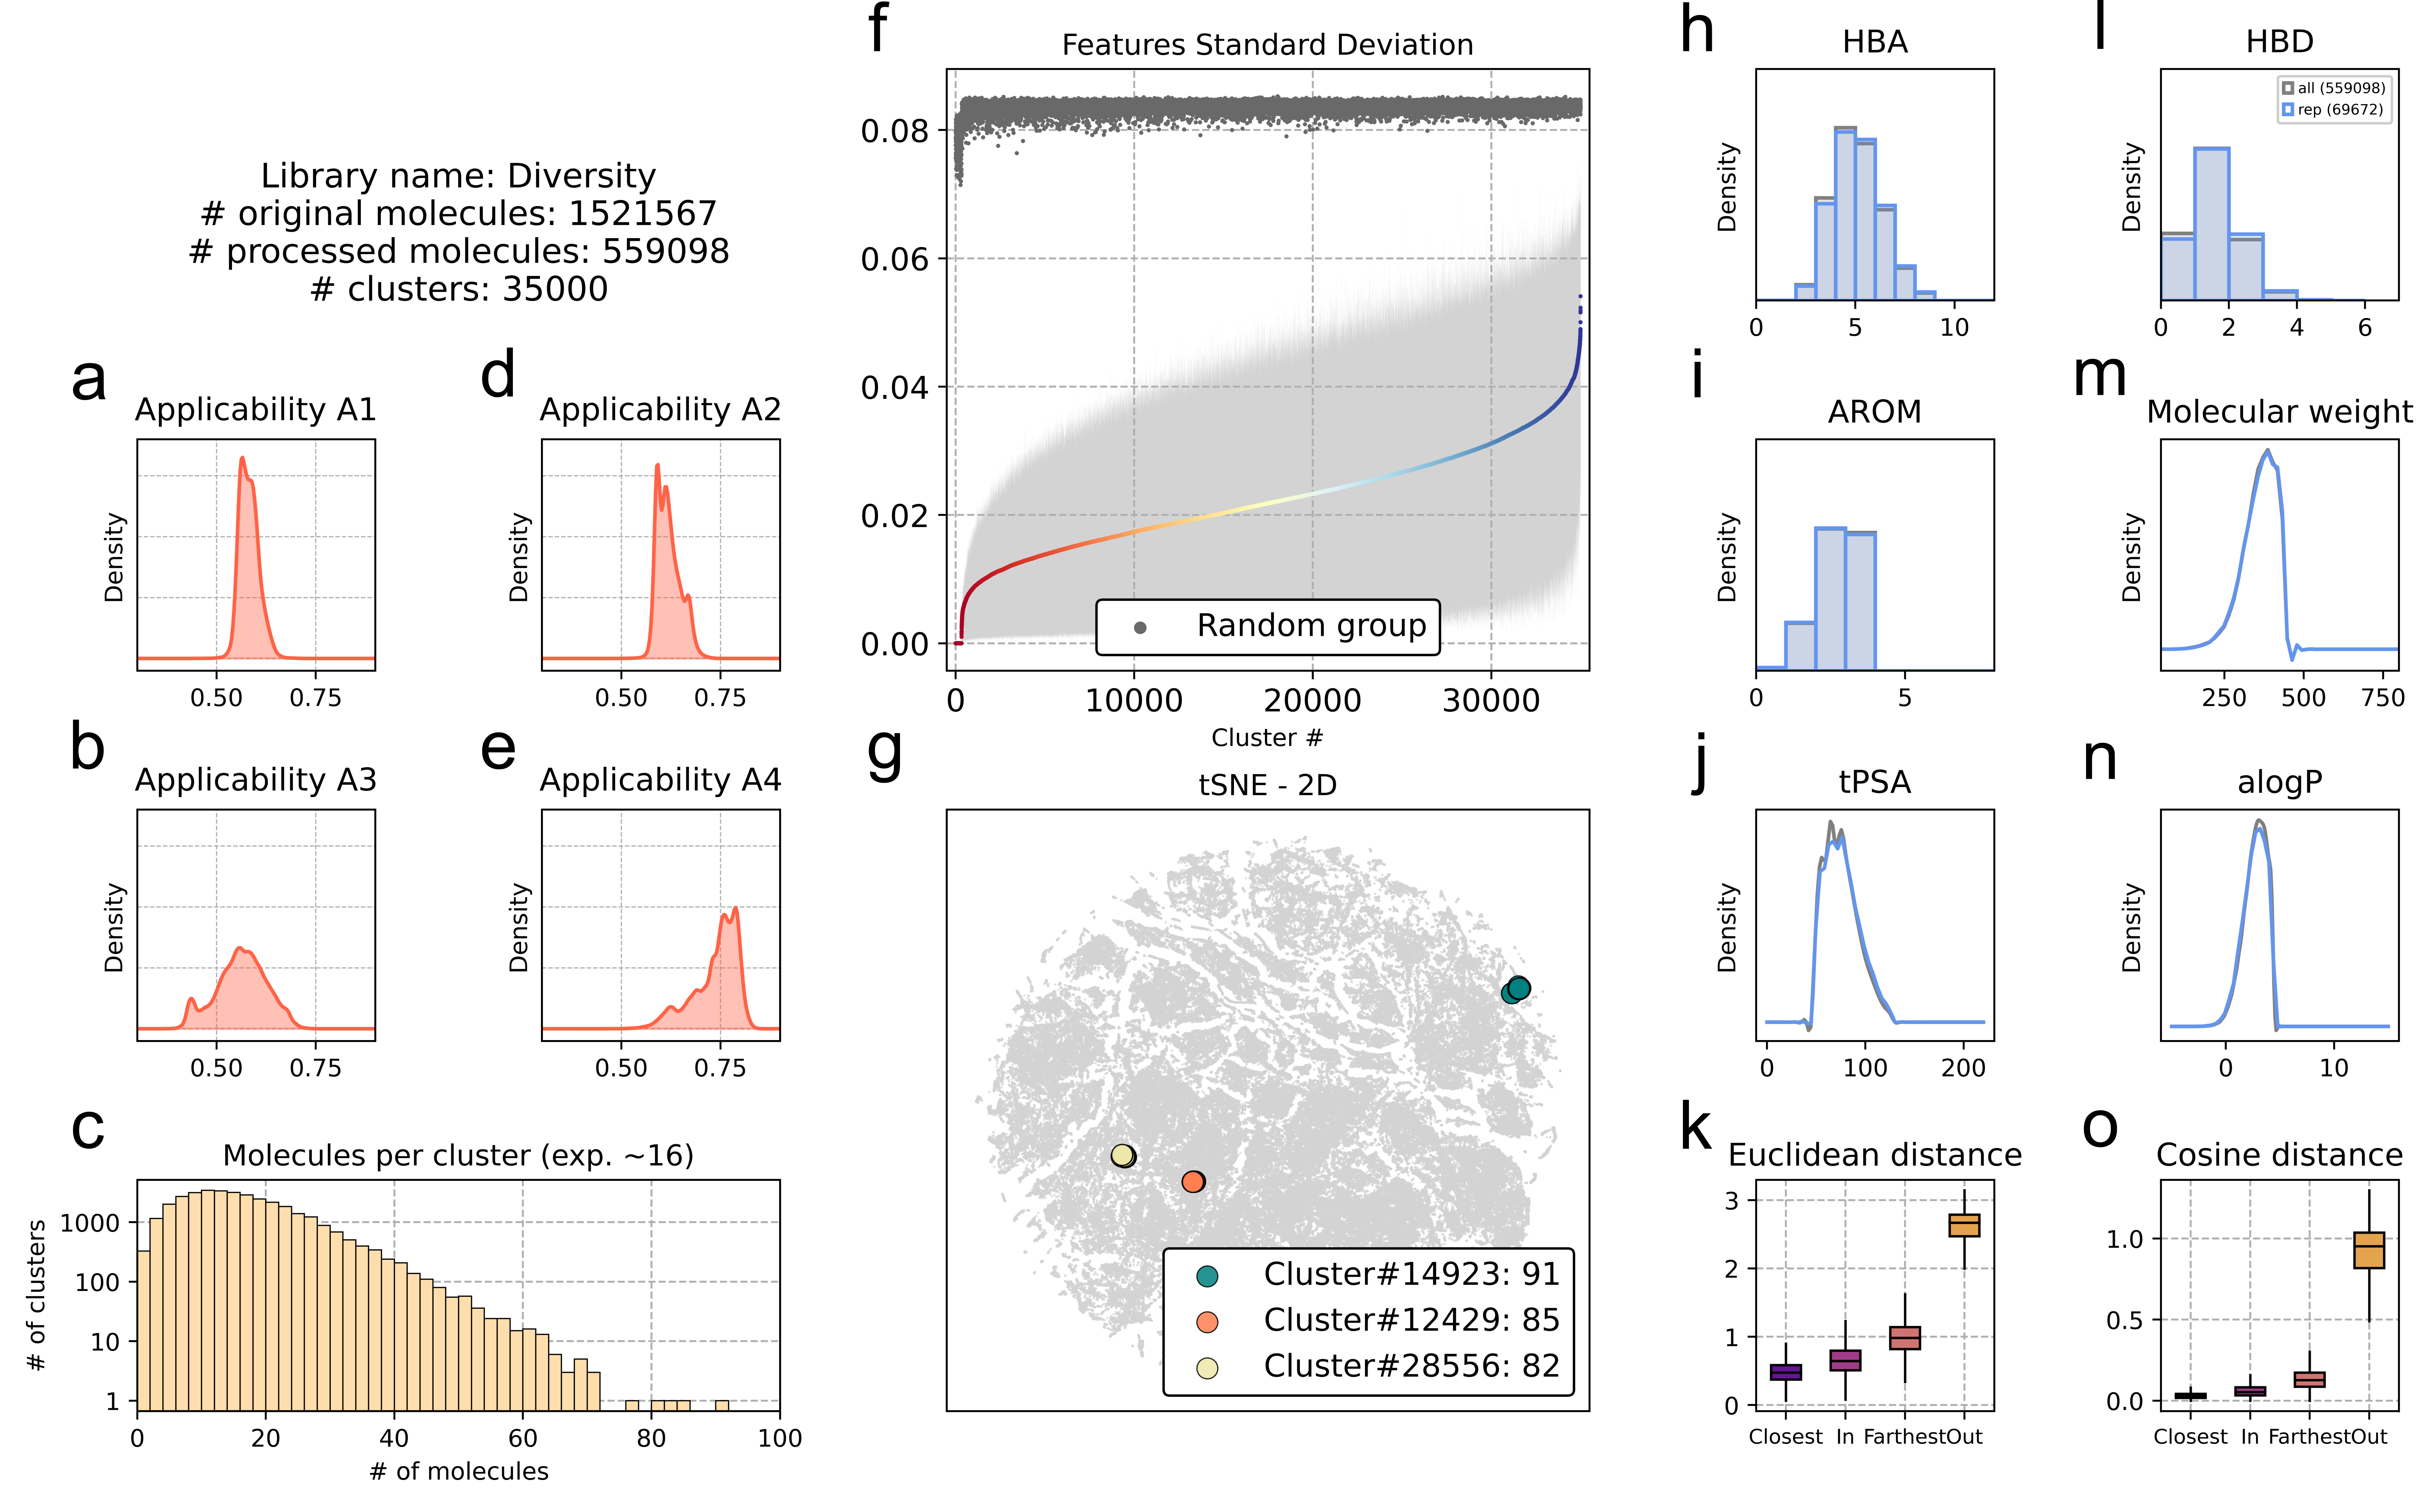
\includegraphics[width=1\linewidth]{figures/Navigation/Main/Diversity_random_v3.png}
  \caption{\textbf{Clustering a chemical library of compounds.}
    \textbf{a,b,d,e)} Distribution of CC signatures’ applicability values for A1, A2, A3 and A4, respectively. 
    \textbf{c)} Number of clusters (y-axis, log scale) having the specified number of molecules (x-axis). The expected number of molecules per cluster is 559k/35k \textasciitilde 16.
    \textbf{f)} For each cluster (x-axis, labeled from 0 to 34,999) standard deviations (y-axis) of the 128 features. Colored points represent the average standard deviation values of the features from signatures within the cluster, light gray bars show the range between the 20\textsuperscript{th} and 80\textsuperscript{th} percentiles of the distribution. Dark gray points represent the average standard deviation values of the features from randomly selected signatures outside the cluster.
    \textbf{g)} 2D tSNE representation of the 559k signaturized compounds (see \hyperref[Navigation_Methods]{Methods}). The top3 most populated clusters are colored accordingly, the legend indicates the number of small molecules within each of these clusters.
    \textbf{h,i,j,l,m,n)} Distributions of number of hydrogen bond acceptors, hydrogen bond donors, aromatic rings, molecular weight, topological polar surface area (tPSA) and alogP for the 559k ChemDiv compounds (after filtering, gray color) and the \textasciitilde70k selected representatives (light blue).
    \textbf{k,o)} Cosine and euclidean distances between the cluster centroid (an abstract 512-dimensional point, see \hyperref[Navigation_Methods]{Methods}) and the nearest compound, the farthest compound and the remaining compounds within each cluster, and a subset of compounds from other clusters.
}
  \vspace{-5mm}
  \rule[0ex]{\textwidth}{0.5pt}
  \vspace{-9mm}
  \label{Navigation_Fig1}
\end{Figure_modified}

\subsubsection{Qualitative visualization of the Chemical Space of small molecules}

To abstractly illustrate the chemical space of small molecules we subsampled compounds from Medina, Metabolights \cite{yurekten_metabolights_2024, haug_metabolights_2019}, CMAUP \cite{zeng_cmaup_2019, hou_cmaup_2024}, RepoHub \cite{corsello_drug_2017}, the Chemical Checker database \cite{duran-frigola_extending_2020} and the in-house chemically diverse IRB Library (herein named Chemical Diversity. Note that we here used the old version of the IRB Library, including 47k compounds). Medina’s natural product library represents one of the largest microbial extract libraries worldwide, providing a unique and invaluable resource for bioactive compound discovery (\hyperlink{https://www.medinadiscovery.com/natural-products-collection/}{https://www.medinadiscovery.com/natural-products-collection/}). On a similar note, Metabolights includes annotated metabolic compounds from various species, while CMAUP provides detailed information on active ingredients of useful medicinal plants. On the other hand, RepoHub (i.e. the Drug Repurposing Hub) is composed of existing clinical and marketed drugs, and is mainly aimed at repurposing known drugs for new therapeutic applications. Additionally, the Chemical Checker database comprises compounds with reported bioactivity in the public domain, and finally, the old version of the IRB proprietary library was specifically designed to maximize chemical diversity, covering a broad area of the synthetic chemical space.

To depict chemical differences between small molecule libraries, we generated chemical CC signatures for all molecules under study (see \hyperref[Navigation_Methods]{Methods}). Such signatures were in fact compact versions (128 dimensions) of state-of-the art chemical fingerprints, including ECFPs (CC A1 space), E3FPs (CC A2), together with embedded Murcko’s scaffold-based representations (CC A3), MACCs Keys (CC A4) and general physicochemical properties (CC A5). Additionally, we also generated bioactivity signatures, i.e. inferred representations of protein binding profiles (CC B4). 

Overall, we observed significant differences in the covered areas of the chemical space when using chemical signatures (A1-A5). For instance, there was very little overlap between compounds from the Chemical Diversity library and natural products from the Medina set (Fig \ref{Navigation_Fig2}). As expected, MetaboLights and CMAUP partially overlapped with Medina, while RepoHub and the Chemical Checker tended to extensively overlap with synthetically diverse compounds. The use of bioactivity signatures (B4) led to the analogous conclusion: natural products and synthetic drugs exhibited distinct protein binding profiles (Fig \ref{Navigation_Fig2}). Indeed, designed drugs and synthetically created compounds are imperfect human inventions with suboptimal properties and bioactivities, usually leading to limited efficacy and undesirable off-target effects. On the other hand, natural products and other ingredients derived from nature have evolved under the pressures of natural selection, resulting in tailored properties and refined selectivity profiles largely owing to their intricate chemical structures. Indeed, the scaffolds covered by synthetic compounds were far simpler than those included in natural products (Fig \ref{Navigation_FigS1}). 



%%%%%%%%%%%%%%%%
%%% FIGURE 2 %%%
%%%%%%%%%%%%%%%%

\begin{Figure_modified}
  \centering
  \includegraphics[width=1\linewidth]{figures/Navigation/Main/ALL_PRETTY.png}
  \caption{\textbf{Chemical space visualization of 6 distinct chemical libraries:} Medina, MetaboLights\cite{yurekten_metabolights_2024, haug_metabolights_2019}, CMAUP\cite{hou_cmaup_2024, zeng_cmaup_2019}, Chemical Diversity, RepoHub\cite{corsello_drug_2017} and the Chemical Checker\cite{duran-frigola_extending_2020}. For each combination of small molecule descriptor (A1-A5 and B4 CC Spaces) and compound library, tSNE 2D representation of the 31,052 generated signatures (see \hyperref[Navigation_Methods]{Methods}). Points are colored by density.
}
  \vspace{-5mm}
  \rule[0ex]{\textwidth}{0.5pt}
  \vspace{-9mm}
  \label{Navigation_Fig2}
\end{Figure_modified}


\subsubsection{The advent of bioactivity signatures}

The use of chemical small molecule descriptors is a common practice in most cheminformatics-related tasks, as we have seen when selecting a representative set of compounds to reduce the size of a large library and also when comprehensively visualizing the chemical space of small molecules. In the latter case, we derived analogous results using bioactivity signatures, which offer a promising framework to explore the chemical space of small molecules in a biologically relevant manner, potentially complementary to the purely chemical view. 

Many drug discovery efforts are rooted in the small molecule similarity principle, stating that structurally similar molecules do exhibit similar bioactivities when exposed to a biological system. Although the principle holds as a general guideline, the relationship between chemical structure and bioactivity is not straightforward and depends on multiple factors that are usually complex to trace. For instance, subtle modifications in a molecular structure may result in the disruption of the binding with its intended target protein or may alter key physicochemical properties, leading to suboptimal pharmacokinetics (e.g. poor absorption).

In the same way as similar molecules may exhibit very distinct bioactivities, non-similar molecules may present similar protein binding profiles. These cases are often overlooked by classical drug discovery efforts that purely rely on the comparison of chemical structures. This is where inferred bioactivity signatures become valuable, as they provide a means to capture functional similarities that are not evident from chemical analysis alone.

To illustrate the potential of bioactivity signatures, we focused our study on the chemical compounds reported to bind to the DNA damage-inducible transcript 3 mouse protein (Uniprot ID: P35639, Gene Name: DDIT3), as documented in the ChEMBL\cite{zdrazil_chembl_2024, gaulton_chembl_2017} database as of March 2024. In brief, we selected the reported active compounds (a total of 572) alongside 10k randomly selected molecules of the CC database, to serve as a background of the chemical space. The use of chemical signatures (CC A1 space, compressed representation of ECFPs) highlighted the diverse nature of these compounds. Remarkably, the binders spanned a wide area of the chemical space (Fig \ref{Navigation_Fig3}a), with cosine distances between them that were essentially indistinguishable from those observed against background compounds (Fig \ref{Navigation_Fig3}b). Although the considerable chemical differences exhibited by known binders, their characterization using bioactivity signatures (CC B4 space, inferred protein binding profiles) was notably more homogeneous. As shown in Fig \ref{Navigation_Fig3}c, most active compounds clustered within a well-defined and specific region of the chemical space due to significantly low distances between them (Fig \ref{Navigation_Fig3}d), emphasizing the high similarity between their bioactivity signatures. 


%%%%%%%%%%%%%%%%
%%% FIGURE 3 %%%
%%%%%%%%%%%%%%%%

\begin{Figure_modified}
  \centering
  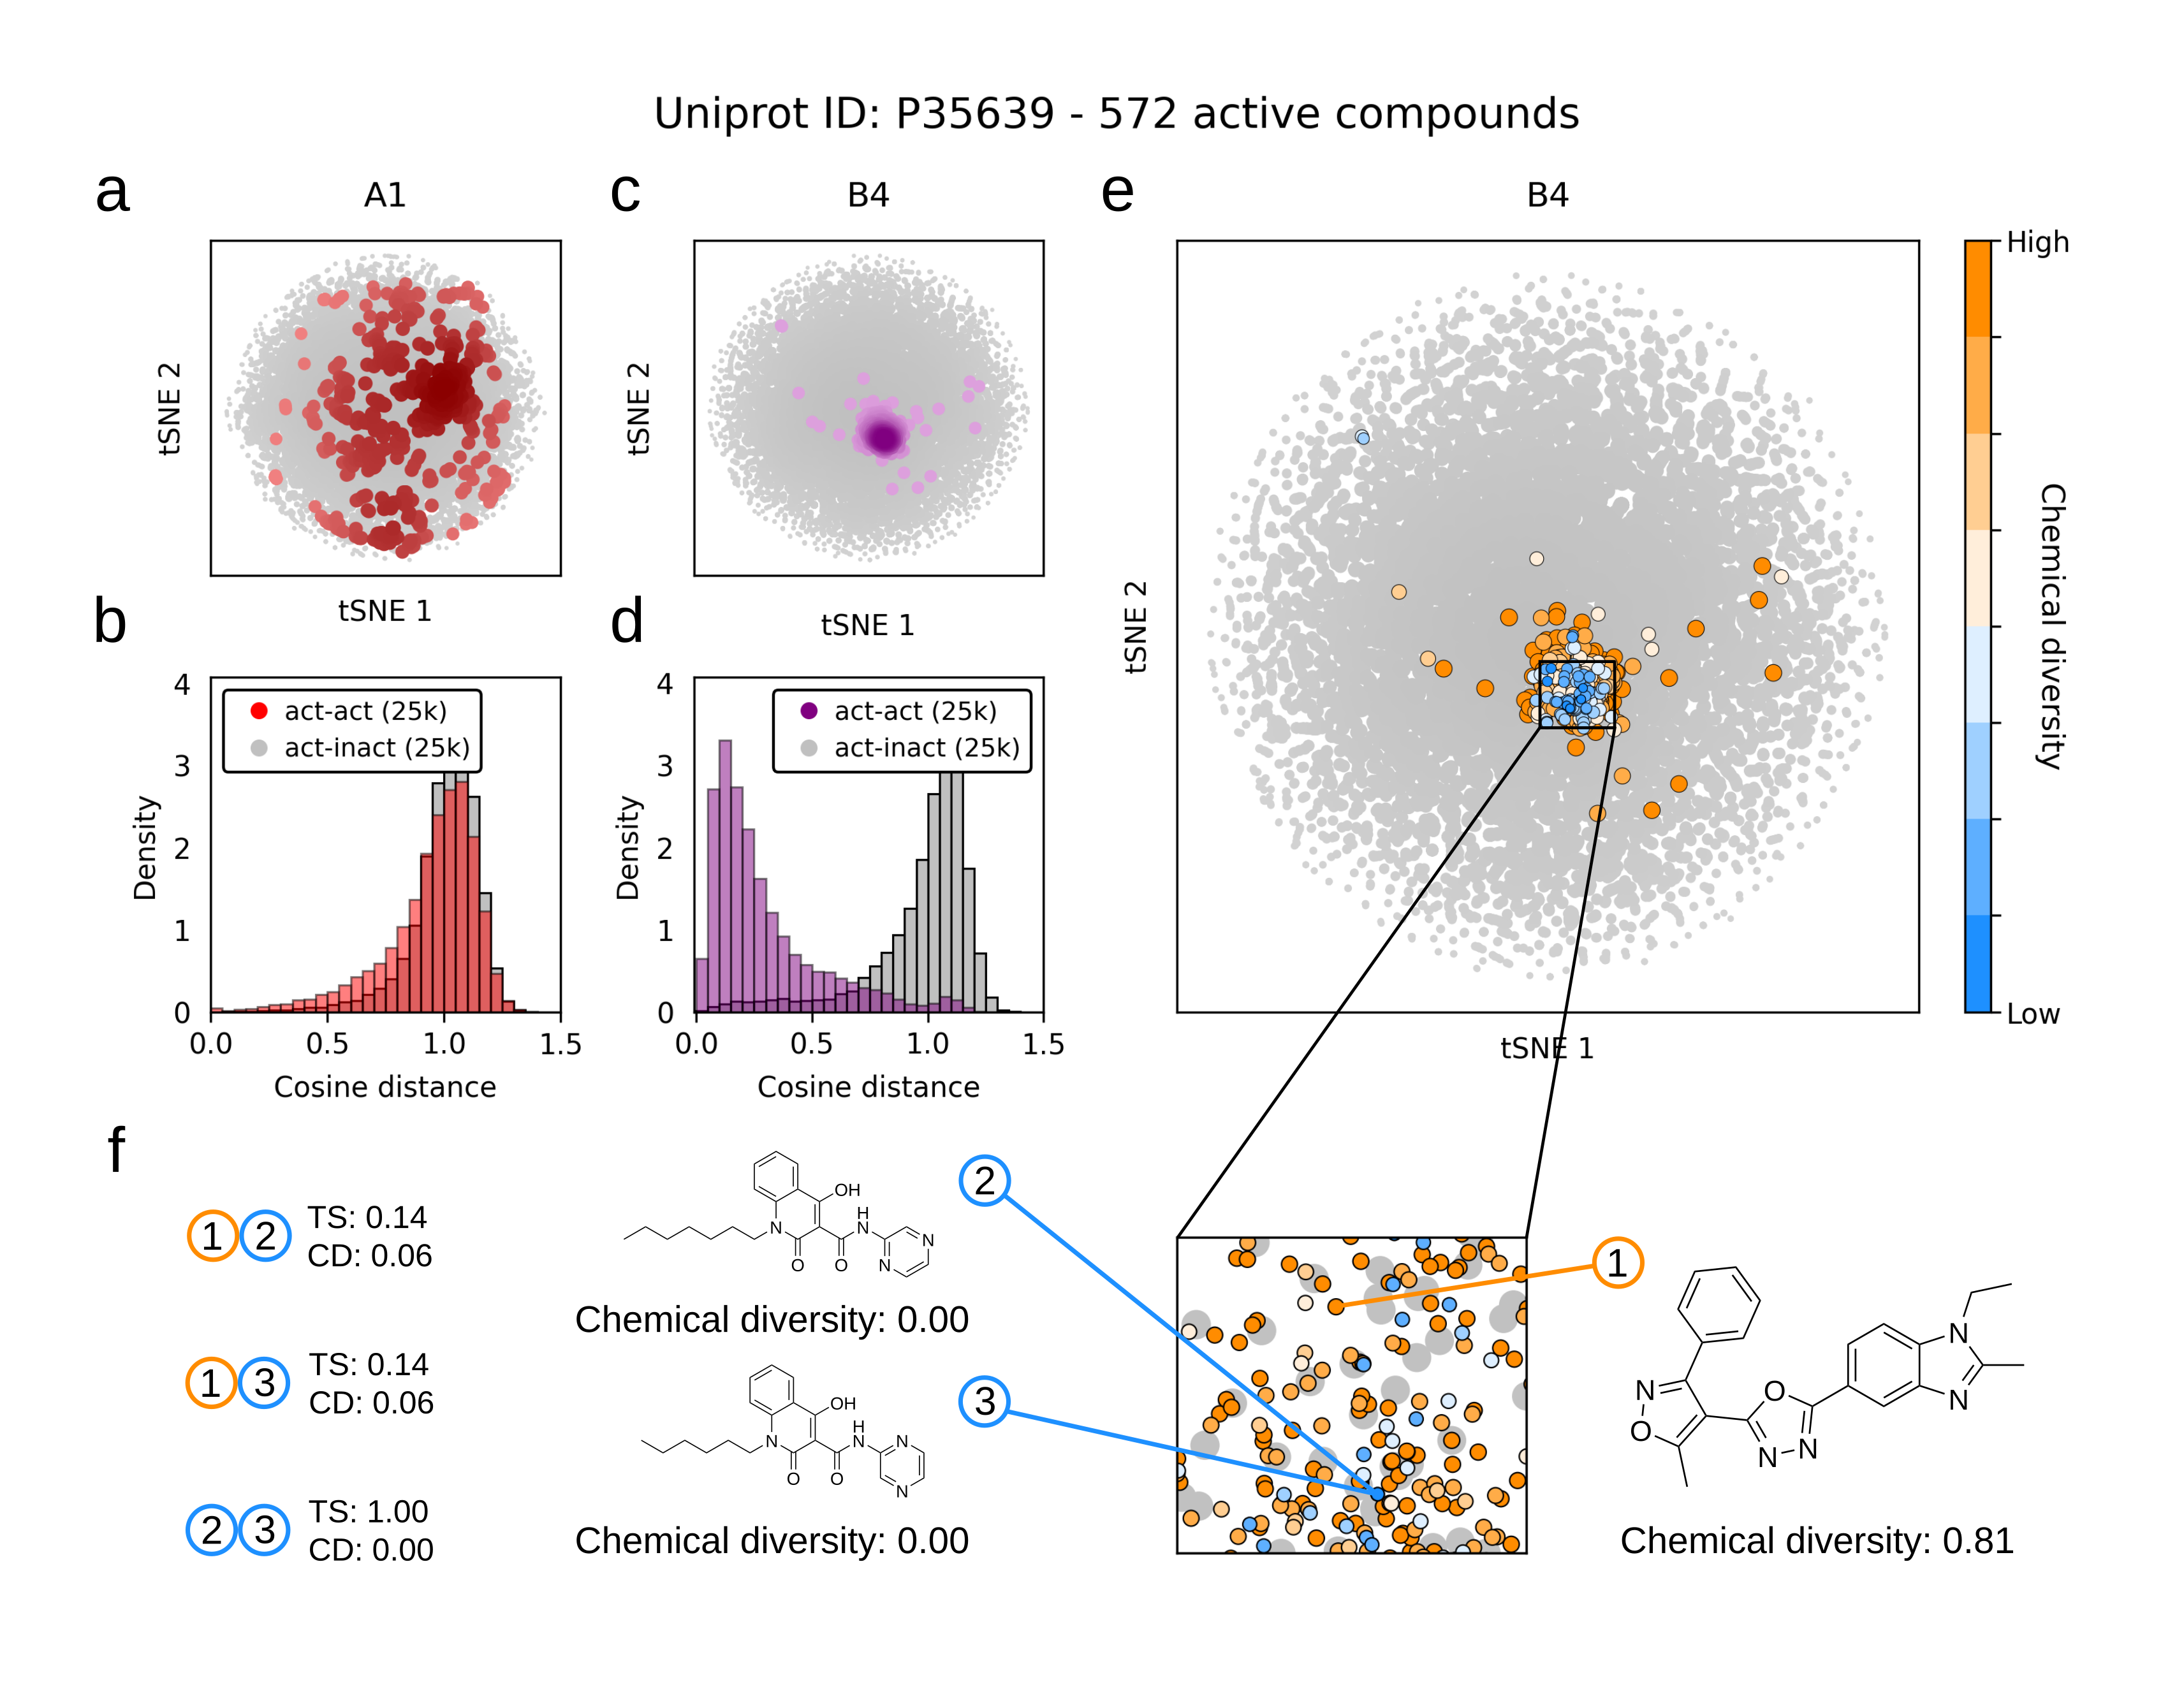
\includegraphics[width=1\linewidth]{figures/Navigation/Main/Fig3_v3.png}
  \caption{\textbf{The advent of bioactivity signatures.}
    \textbf{a)} tSNE 2D representation of the 572 compounds (red, colored by density) reported to be active against P35639 (Uniprot ID, Gene Name: DDIT3) in the CC database (v.2024) derived from ChEMBL and BindingDB. Gray dots correspond to 10k randomly selected compounds that serve as a background of the chemical space. All compounds were previously characterized using the CC A1 signaturizer\cite{bertoni_bioactivity_2021}.
    \textbf{b)} Distribution of cosine distances between active compounds (red, 25k subsampled comparisons) and between active and inactive compounds (gray, 25k subsampled comparisons). All compounds were previously characterized using the CC A1 signaturizer\cite{bertoni_bioactivity_2021}.
    \textbf{c)} tSNE 2D representation of the 572 compounds (purple, colored by density) reported to be active against P35639 (Uniprot ID, Gene Name: DDIT3) in the CC database (v.2024) derived from ChEMBL and BindingDB. Gray dots correspond to 10k randomly selected compounds that serve as a background of the chemical space. All compounds were previously characterized using the CC B4 signaturizer\cite{bertoni_bioactivity_2021}.
    \textbf{d)} Distribution of cosine distances between active compounds (purple, 25k subsampled comparisons) and between active and inactive compounds (gray, 25k subsampled comparisons). All compounds were previously characterized using the CC B4 signaturizer\cite{bertoni_bioactivity_2021}.
    \textbf{e)} tSNE 2D representation of the 572 compounds (colored by chemical diversity, see Methods) reported to be active against P35639 (Uniprot ID, Gene Name: DDIT3) in the CC database (v.2024) derived from ChEMBL and BindingDB. In short, the chemical diversity value represents the chemical redundancy from the neighboring environment of a bioactivity signature. Gray dots correspond to 10k randomly selected compounds that serve as a background of the chemical space. All compounds were previously characterized using the CC B4 signaturizer\cite{bertoni_bioactivity_2021}.
    \textbf{f)} A defined region of the chemical space (see previous subplot) is zoomed in to show (i) a compound having a high chemical diversity value (orange) as well as (ii) a pair of compounds having low chemical diversity (high chemical redundancy, blue). TS: Tanimoto Similarity. CD: Cosine Distance. 
}
  \vspace{-5mm}
  \rule[0ex]{\textwidth}{0.5pt}
  \vspace{-9mm}
  \label{Navigation_Fig3}
\end{Figure_modified}


To provide further insights into these results, we assigned a numerical value to each of the 572 compounds representing the chemical diversity captured in their neighboring environment (see \hyperref[Navigation_Methods]{Methods}). In brief, the value illustrated how chemically similar a reference molecule was to those compounds having highly similar bioactivity signatures (top-10 NN). As shown in Fig \ref{Navigation_Fig3}e, active compounds had varying values of chemical diversity, ranging from low (blue, Tanimoto Similarities \textasciitilde 1) to high (orange, Tanimoto Similarities \textasciitilde 0.15) values. We then selected three representative compounds as exemplary cases to further illustrate these findings (Fig \ref{Navigation_Fig3}f). Compound \#1, with a diversity value of 0.81, exemplifies a significant chemical variation compared to its bioactivity-similar neighbors. In other words, compound \#1 was chemically different from its top-10 bioactivity-neighbors. On the other hand, compounds \#2 and \#3 represented the opposite case, having top-10 NNs with a maximum Tanimoto Similarity of 1 (leading to a chemical diversity value of 0). In fact, compound \#2 was the NN of compound \#3, and vice versa, pinpointing their nearly identical structures, differing only in the number of carbons in the aliphatic chain. 

Overall, these results highlight the impact that inferred bioactivity signatures may have in the context of drug discovery, offering an alternative framework to navigate the chemical space in an optimal manner for biological applications. In particular, a classical approach based on chemical features and descriptors, would have correctly anticipated the existing relationship between compounds \#2 and \#3 in terms of protein-ligand binding. However, chemical signatures alone would have failed to meaningfully relate compounds \#2 and \#3 with compound \#1. By leveraging bioactivity signatures, similarities between compounds \#1 and \#2 (or \#3) become significant (cosine distance of 0.06), and would have been anticipated even in the absence of chemical similarity (Tanimoto Similarity of 0.14). 

\subsection{Concluding remarks}


Bla bla bla


\subsection{Methods}
\label{Navigation_Methods}


Bla bla bla


\newpage


%%%%%%%%%%%%%%%%%
% STEREOISOMERS %
%%%%%%%%%%%%%%%%%

\section[Stereochemically-aware bioactivity descriptors for uncharacterized chemical compounds]{Chapter 3.3 -- Stereochemically-aware bioactivity descriptors for uncharacterized chemical compounds}
\label{Chapter_3.3}
\setcounter{figure}{0}
\renewcommand{\thefigure}{3.\arabic{section}.\arabic{figure}}
\hspace*{\fill} Work published in Journal of Cheminformatics. \newline
\hspace*{\fill} Publication \#2, see the \hyperref[ListOfPublications]{List of publications}.
% \addcontentsline{toc}{section}{Chapter 3.3 -- Stereoisomers}
\subsection{Abstract}

Stereochemistry plays a fundamental role in pharmacology. Here, we systematically investigate the relationship between stereoisomerism and bioactivity on over 1M compounds, finding that a very significant fraction (\textasciitilde40\%) of spatial isomer pairs show, to some extent, distinct bioactivities. We then use the 3D representation of these molecules to train a collection of deep neural networks (Signaturizers3D) to generate bioactivity descriptors associated to small molecules, that capture their effects at increasing levels of biological complexity (i.e. from protein targets to clinical outcomes). Further, we assess the ability of the descriptors to distinguish between stereoisomers and to recapitulate their different target binding profiles. Overall, we show how these new stereochemically-aware descriptors provide an even more faithful description of complex small molecule bioactivity properties, capturing key differences in the activity of stereoisomers.




\subsection{Introduction}


Small molecules are a great tool to probe biology and, still, the main asset of pharmaceutical companies. The last years have seen a surge of ever more complex biological high-throughput assays involving the use of chemical compounds, and databases committed to gathering bioactivity data associated to small molecules are expanding \cite{zdrazil_chembl_2024, kim_pubchem_2023}. Moreover, the widespread availability of computational resources\cite{tetko_bigchem_2016} and artificial intelligence techniques has been pivotal to leverage such amounts of data\cite{von_lilienfeld_retrospective_2020}. 

From the computational perspective, small molecules are typically characterized by numerical descriptors encoding physicochemical or topological features\cite{fernandez-torras_connecting_2022}. Compounds can be further described using their biological activities (e.g. the targets they interact with), which represents a complementary strategy that extends the small molecule similarity principle beyond conventional chemical properties\cite{duran-frigola_extending_2020}. Unfortunately, experimental bioactivity data are sparse and only available for a limited set of well-characterized compounds. To overcome these coverage issues, we recently trained a collection of deep neural networks able to infer bioactivity signatures for any compound of interest (i.e. Signaturizers), even when little or no experimental information is available for them\cite{bertoni_bioactivity_2021}. The Signaturizers are able to infer 25 different bioactivity types, from target profiles to cellular responses or clinical outcomes. However, the original Signaturizers are built on 2D representations of molecules and are thus not able to capture subtle, but often meaningful, bioactivity differences between stereoisomers. Indeed, stereochemistry and chirality play pivotal roles in pharmacology\cite{scott_stereochemical_2022, h_brooks_significance_2011}, often driving supramolecular recognition processes crucial in drug design. Biological matter is intrinsically chiral\cite{inaki_cell_2016} (e.g. amino acids) and stereoisomeric small molecule drugs may exhibit different therapeutic and toxicological effects\cite{mcconathy_stereochemistry_2003, smith_chiral_2009}. For example, the antidepressant Citalopram is administered as a mixture of two enantiomers (i.e. racemate), although only one of them is pharmacologically active\cite{snchez_escitalopram_2004, sanchez_pharmacology_2006}. However, in some other cases, one of the enantiomers is associated with toxic side effects. This is the case of the antiarthritic drug Penicillamine, administered as an enantiomerically pure compound ((S)-Penicillamine) since (R)-Penicillamine acts as a pyridoxine (vitamin B6) antagonist and is thus toxic\cite{smith_chiral_2009, williams_enantiomers_1990}. We now present novel deep learning models to generate stereochemically-aware bioactivity signatures for any compound of interest, which we call Signaturizers3D, that overcome the inherent limitations of our original Signaturizers. 


\subsection{Results and discussion}


%%%%%%%%%%%%%%%%%%%%%%%%%%%%%%%%%%%%%%%%%%%%%%%%%%%%%%%%%%%%%%%%
%%  Systematic quant. of the relationship between stereo. and small molecule bioactivity
%%%%%%%%%%%%%%%%%%%%%%%%%%%%%%%%%%%%%%%%%%%%%%%%%%%%%%%%%%%%%%%%

\phantomsection
\subsubsection{Systematic quantification of the relationship between stereochemistry and small molecule bioactivity}
\label{Stereoisomers_Rel_Stereo_Bioactivity}


The first steps in the development of Signaturizers3D were (i) to select a comprehensive database containing detailed bioactivity data for a wide range of chemical compounds, and (ii) within this database, systematically identify groups of stereoisomers to compare their bioactivity profiles and evaluate the ability of Signaturizers3D to distinguish them.
To gather bioactivity data, we used the Chemical Checker (CC), which represents the largest collection of small molecule bioactivity signatures available to date, with experimental information for over 1M compounds\cite{duran-frigola_extending_2020}. \hl{The CC divides data into five levels of increasing complexity, ranging from the chemical properties of compounds to their clinical outcomes. Compound bioactivities are expressed in a vector-like format (i.e. signatures), and the data processing pipeline also includes several steps of increasing level of integration and abstraction: from raw experimental data representing explicit knowledge (type 0 signatures) to inferred representations that leverage all the experimentally determined bioactivities available for each molecule (type III signatures).} Thus, we processed the whole CC (i.e. 25 different bioactivity types for about 1M molecules) to systematically identify groups of stereoisomers that might exhibit distinct bioactivities. In brief, we first identified stereoisomers using their InChIKey strings and we then applied several filters to ensure that the actual differences between compounds were exclusively due to stereochemical variations (see \href{Stereoisomers_Methods}{Methods} for further details). Then, we selectively removed molecules that were not exhaustively characterized, in order to work with enantiomerically pure compounds and prevent the analysis of results derived from racemic mixtures (Fig 1a). We eventually identified 23,830 groups of stereoisomers, involving 57,989 compounds, across the different CC bioactivity spaces. We found most stereoisomeric groups with experimental information in the target binding space (B4) and in the network spaces derived from B4 (i.e. C3-5, Fig S1). We thus focused our study on the B4 space, which contains over 600,000 molecules, and we identified 15,370 groups of stereoisomers, involving 32,705 compounds (Fig 1b). We then analyzed the binding profiles for all these compounds, and found 6,022 groups that had at least 2 stereoisomers with non-identical binding profiles. We also observed that the majority of the groups (14,181, ~92%) contained only 2 stereoisomers (Fig 1c, top), in 38% of which both compounds showed distinct binding profiles (Fig 1c, bottom). Analogously, we identified 562 groups containing 3 stereoisomers: 230 (41%), 195 (35%) and 137 (24%) of them showing 1, 2 and 3 distinct binding profiles, respectively. Finally, we observed that the distribution of Jaccard distances between binding profiles within stereoisomeric groups was skewed towards low values (i.e. more similar profiles) compared with random pairs, while pairs of compounds sharing at least one target were somewhere in the middle (Fig 1d). Fig 1e shows, as an illustrative example, a group of 3 stereoisomers with non-identical binding profiles, where compounds A and C weakly and strongly bind with the Beta-1 adrenergic receptor (ADRB1; 2nd position in the profile), respectively, whilst compound B does not bind it. Note that inactive compound-target interactions might be false negatives due to, for instance, a limited sensitivity of the detection methods or non-tested enantiomers.


\begin{Figure_modified}
  \centering
  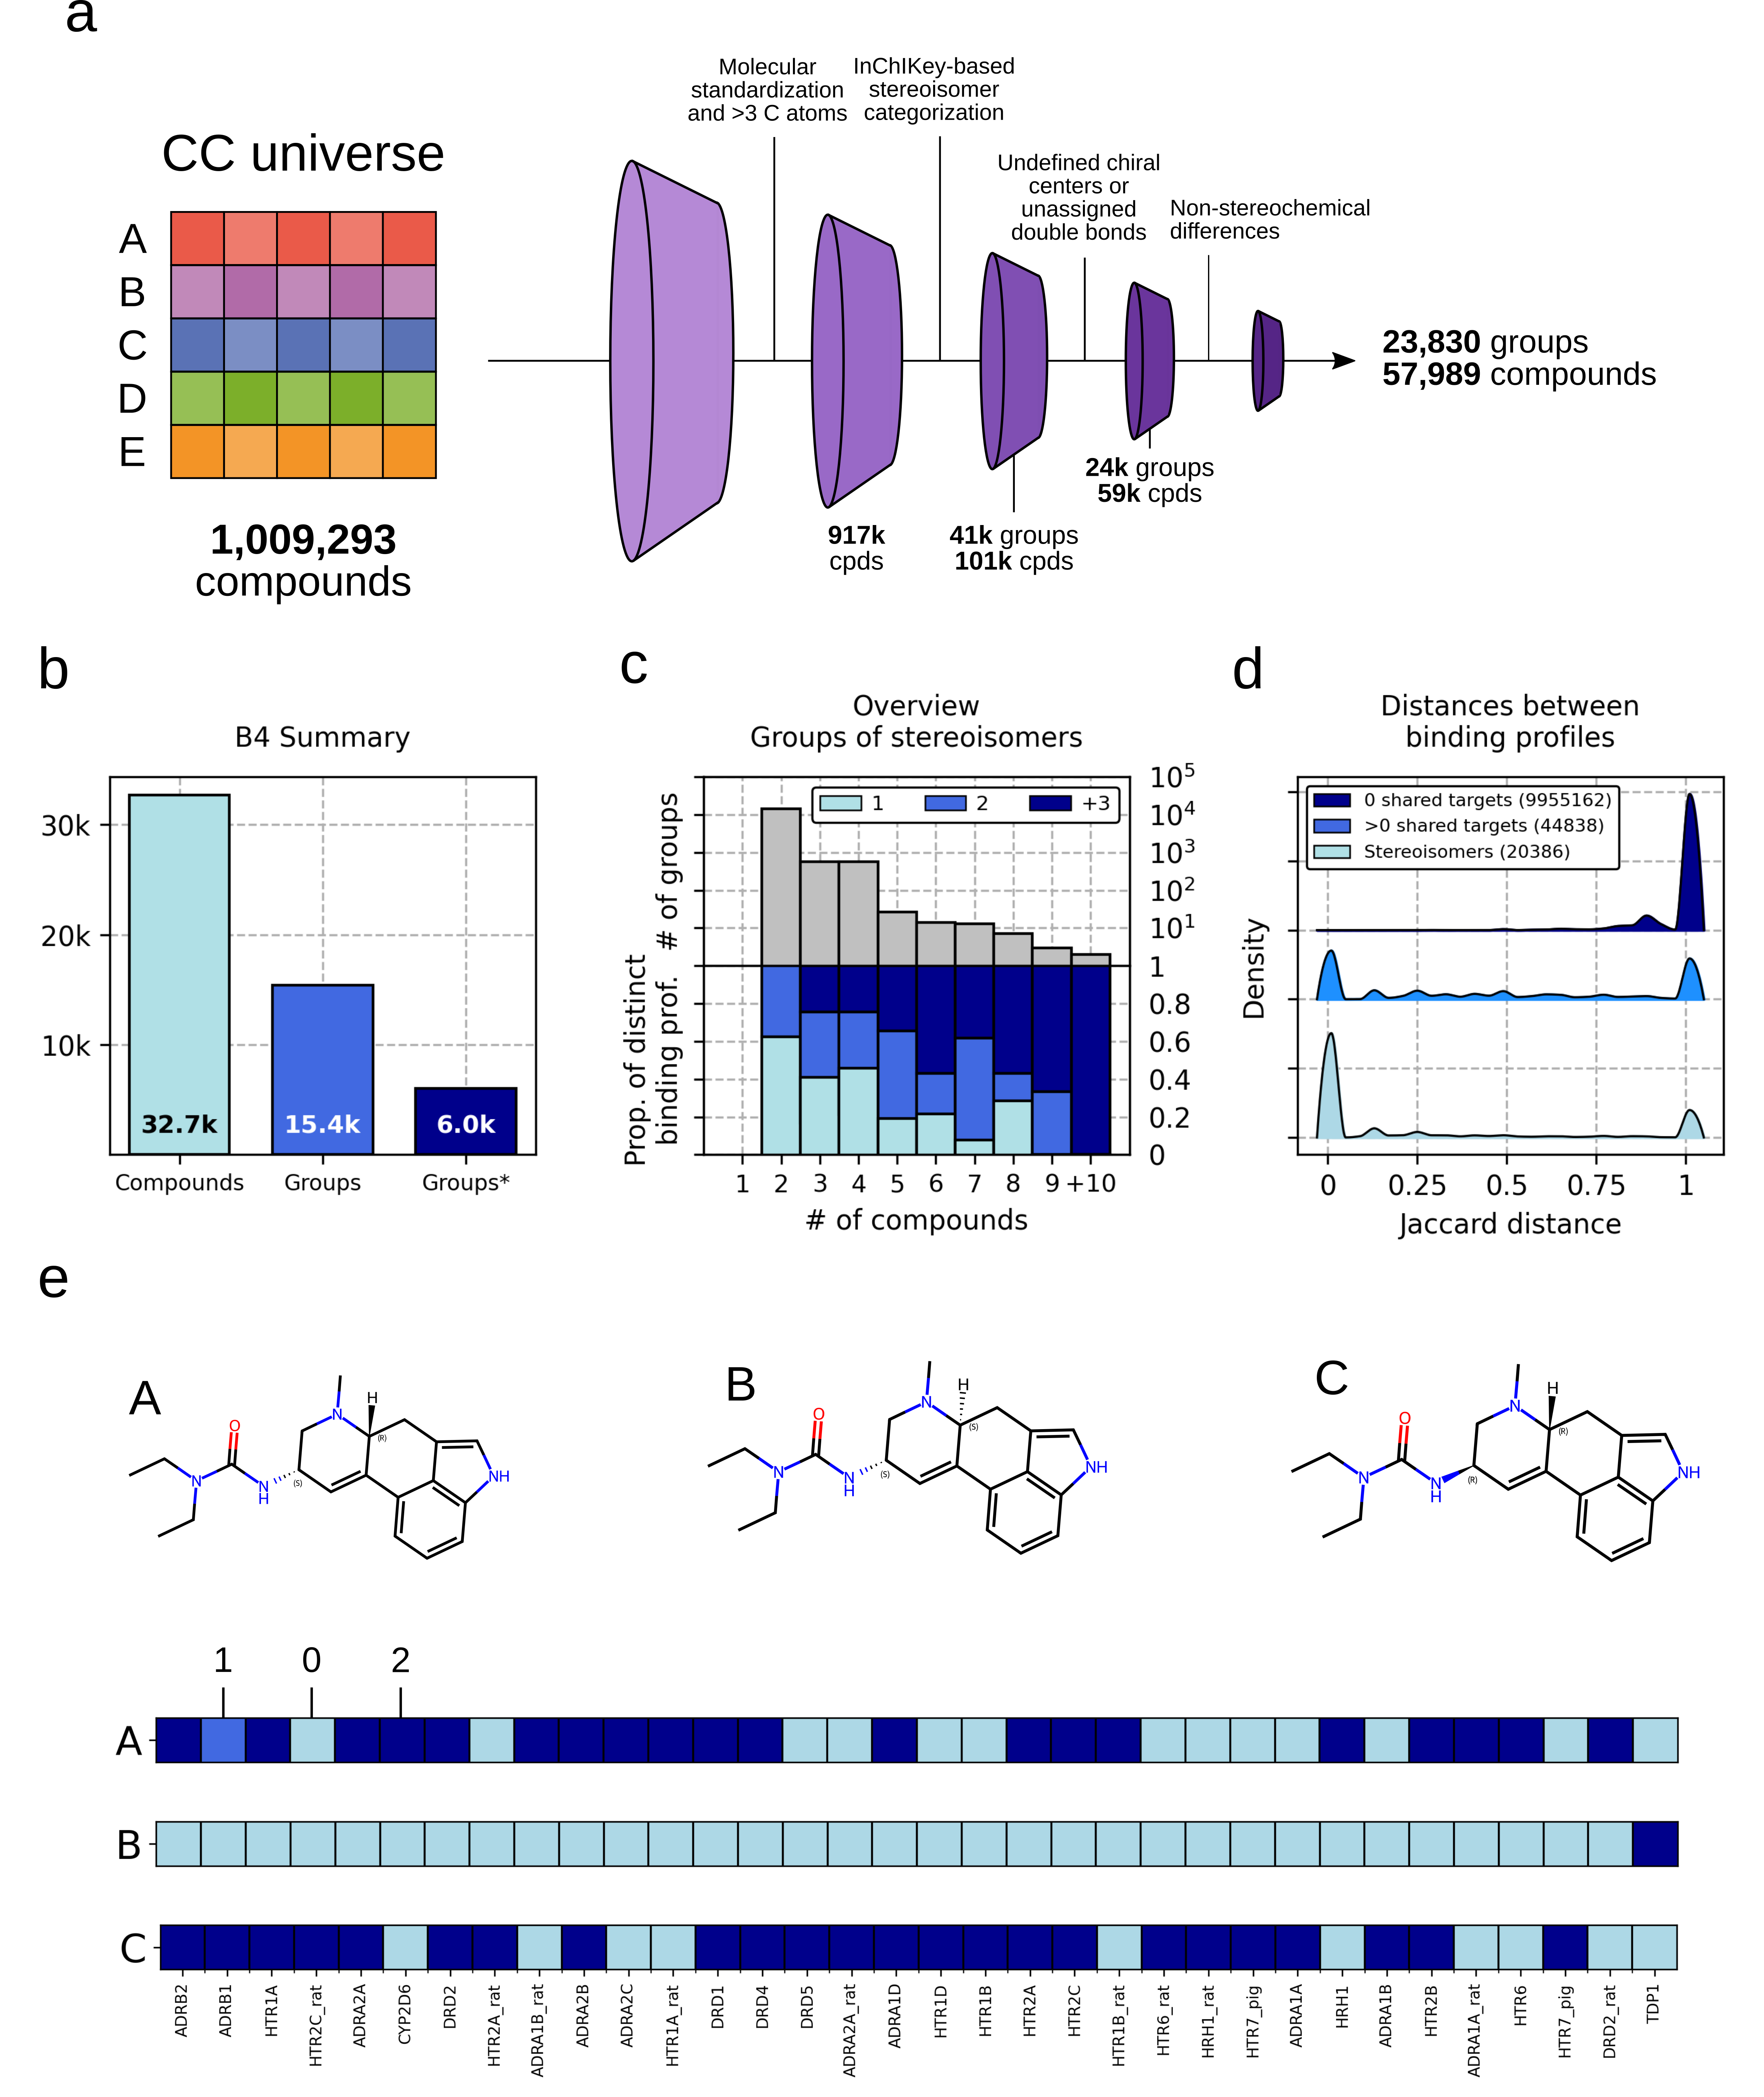
\includegraphics[width=1\linewidth]{figures/Stereoisomers/Main/Fig1_v2.png}
  \caption{
    \textbf{Stereoisomerism and bioactivity.}
    \textbf{a)} Computational pipeline to identify groups of stereoisomers in the CC chemical universe.
    \textbf{b)} Number of unique stereoisomeric compounds with experimentally identified protein targets in the CC B4 space, number of stereoisomer groups, and number of groups with at least 2 compounds with non-identical binding profiles.
    \textbf{c)} Number of groups (y-axis, top) having the specified number of stereoisomers (x-axis). Proportion of these groups (y-axis, bottom) having the specified number of distinct binding profiles (i.e. \textasciitilde60\% of the groups of 2 isomers have a unique binding profile).
    \textbf{d)} Distributions of Jaccard distances (binding profiles) between pairs of compounds sharing 0, ≥1 targets and stereoisomer pairs. All distributions are significantly different from each other (Mann-Whitney p-value\textasciitilde0).
    \textbf{e)} Illustrative example of a stereoisomer group including 3 small molecules with their corresponding target binding profiles, using the annotation of type 0 signatures (i.e. 0: no binding; 1: weak binding and 2: strong binding).
    \rule[0ex]{\textwidth}{0.5pt}
  }
  \label{Stereoisomers_Fig1}
\end{Figure_modified}
\subsection{Code and data availability}
\label{Stereoisomers_Code}

An open source Python package to generate 3D-aware CC bioactivity signatures is available at \href{https://gitlabsbnb.irbbarcelona.org/packages/Signaturizer3d}{https://gitlabsbnb.irbbarcelona.org/packages/Signaturizer3d}. The package includes model weights for each of the 25 CC spaces and can be used to characterize molecules using SMILES or coordinates from existing conformers as input. The models are implemented in Pytorch and support inference on a GPU or CPU. The average time to generate CC signatures from SMILES is 16.3s per 1,000 molecules on an NVIDIA GeForce RTX 3090.


\subsection{Concluding remarks}

We have systematically assessed the relationship between stereoisomerism and bioactivity on a large scale, focusing on compound-target binding events. Subsequently, we used our findings to train the second generation of Signaturizers, which are now stereochemically-aware, thereby providing an even more faithful and accurate representation of complex small molecule bioactivity properties.

\subsection{Methods}
\label{Stereoisomers_Methods}

\phantomsection
\subsubsection{Identification of stereoisomers in the CC universe}

We first downloaded small molecule bioactivity data from the official CC website (\hyperlink{https://chemicalchecker.com/downloads/signature0}{https://chemicalchecker.com/downloads/signature0}, 25 spaces). We standardized a total number of\\ 1,009,293 compounds (InChIs) using the standardiser package (\hyperlink{https://github.com/flatkinson/standardiser/tree/master}{https://github.com/flatkinson/standardiser/tree/master}; removal of solvent and salt molecules, charge neutralization and application of tautomeric rules), leading to 916,931 standardized and neutral small molecules having 3 or more carbon atoms. Subsequently, we identified groups of stereoisomers based on their InChIKeys\cite{heller_inchi_2015}, generated using RDKit (\hyperlink{https://www.rdkit.org}{https://www.rdkit.org}). For compounds to be categorized in the same group, they needed to have identical first blocks (indicating identical connectivities between atoms) and non-identical second blocks (indicating differences in stereochemistry, isotopic atoms, the InChI version, etc). In addition, we excluded small molecules with unspecified chiral centers or unassigned double bond configurations. Finally, we also removed compound pairs having different InChIs after stereochemical information was deleted using RDKit, such as pairs with distinct isotopes. We only conserved groups having ≥2 compounds. Overall, we identified 23,830 groups of stereoisomers, including 57,989 compounds. A graphical scheme of the pipeline is shown in Fig \ref{Stereoisomers_Fig1}a.


\phantomsection
\subsubsection{Training and evaluation of Signaturizers3D}

For all molecules in the CC, we generated and optimized a single 3D conformation per compound using the ETKDG method\cite{riniker_better_2015} and the Merck Molecular Force Field (MMFF94) from RDKit, respectively, with hydrogens included. We successfully generated conformations for \textasciitilde99\% of the compounds (998,186). The rest, mostly very large molecules, were excluded from the final dataset. We then did 80/20 scaffold-based splits (x3) of the 998,186 considered compounds.
After removing hydrogens, all coordinates and atom-types for each molecule were used to fine-tune the pre-trained Uni-Mol model as a multitarget regression problem, so that we could directly infer pre-calculated CC type III signatures (128 dimensions). Uni-Mol pre-trained model was directly downloaded from \hyperlink{https://github.com/dptech-corp/Uni-Mol/releases/download/v0.1/mol_pre_no_h_220816.pt}{https://github.com/dptech-corp/Uni-Mol/releases/download/v0.1/mol\_pre\_no\_h\_220816.pt}, which provided the initial weights and defined the model’s architecture. To fine-tune the existing Uni-Mol model, we trained for 40 epochs with a batch size of 32 and a learning rate of 0.0001 (warm up ratio of 0.06 without dropout). We used the Adam optimizer with betas (0.9, 0.99) and epsilon 10-6, and we utilized a polynomial decay scheduler for the learning rate. Models were trained on the previously generated scaffold-based splits (3x25, 80/20) using a smooth mean absolute error loss for function optimization. Validation was based on the aggregated mean absolute error (\textit{valid\_agg\_mae}), with early stopping after 20 epochs if no improvement was observed. Training was executed on a GPU with mixed precision (FP16). 

\phantomsection
\subsubsection{K-nearest neighbors recovery}

First, we needed to establish a distance cutoff to eventually define positive pairs of compounds (nearest neighbors) at type III signature level. To do so, we sampled 10k molecules in each of the 25 bioactivity spaces and, after calculating the full pairwise distance matrix between these compounds (10\textsuperscript{8} distances within each space), we established the NN cutoff distance as the 0.001 percentile of the distribution. In this way, a distance cut-off was defined for each CC space. 
Positive pairs (NN) for a given compound at type III signature level were defined as those compounds being at a distance lower than the established cutoff for each CC space. For the strict NN recovery, negative pairs (not NN) were defined as those being at a distance greater than the established cutoff but lower than three times the cutoff distance. The ratio of negative to positive pairs was capped at 10:1. We calculated distances between compounds using Signaturizers and Signaturizers3D for all (x3) scaffold-based 80/20 splits, and we assessed their ability to recapitulate NNs at type III signature level by calculating the corresponding ROC Curves with a subsample of 1k molecules per space. Analogously, positive pairs (NN) for a given compound at B4 type 0 signature level were defined as those compounds having identical target binding profiles (corresponding to a p-value \textasciitilde10\textsuperscript{-3}). For the strict NN recovery, negative pairs (not NN) were defined as those having a Jaccard distance <0.6 (any pair with a Jaccard distance >0 was accepted as negative in the classical NN recovery exercise). We calculated distances between compounds using Signaturizers and Signaturizers3D and we assessed their ability to recapitulate NNs at type 0 signature level by calculating the corresponding ROC Curves with x10 subsamples of 2.5k molecules.
\newpage


%%%%%%%%%%%%%%%%%
%%% POCKETVEC %%%
%%%%%%%%%%%%%%%%%


\section[Comprehensive detection and characterization of human druggable pockets through novel binding site descriptors]{Chapter 3.4 -- Comprehensive detection and characterization of human druggable pockets through novel binding site descriptors}
% \addcontentsline{toc}{section}{Chapter 3.4 -- Comprehensive detection and characterization of human druggable pockets through novel binding site descriptors}
\label{Chapter_3.4}
\setcounter{figure}{0}
\renewcommand{\thefigure}{3.\arabic{section}.\arabic{figure}}
% \hspace*{\fill} Work published in Nature Communications.  \newline \newline
\textbf{Work published in Nature Communications.}

\textbf{Comajuncosa-Creus, A.}, Jorba, G., Barril, X. and Aloy, P., 2024. Comprehensive detection and characterization of human druggable pockets through binding site descriptors. Nature Communications, 15(1), pp.1-20.

\subsection{Abstract}

% Druggable pockets are protein regions that have the ability to bind organic small molecules, and their characterization is essential in target-based drug discovery. However, strategies to derive pocket descriptors are scarce and usually exhibit limited applicability. Here, we present PocketVec, a novel approach to generate pocket descriptors for any protein binding site of interest through the inverse virtual screening of lead-like molecules. We assess the performance of our descriptors in a variety of scenarios, showing that it is on par with the best available methodologies, while overcoming some important limitations. In parallel, we systematically search for druggable pockets in the folded human proteome, using experimentally determined protein structures and AlphaFold2 models, identifying over 32,000 binding sites in more than 20,000 protein domains. Finally, we derive PocketVec descriptors for each small molecule binding site and run an all-against-all similarity search, exploring over 1.2 billion pairwise comparisons. We show how PocketVec descriptors facilitate the identification of druggable pocket similarities not revealed by structure- or sequence-based comparisons. Indeed, our analyses unveil dense clusters of similar pockets in distinct proteins for which no inhibitor has yet been crystallized, opening the door to strategies to prioritize the development of chemical probes to cover the druggable space.

Druggable pockets are protein regions that have the ability to bind organic small molecules, and their characterization is essential in target-based drug discovery. However, deriving pocket descriptors is challenging and existing strategies are often limited in applicability. We introduce PocketVec, an approach to generate pocket descriptors via inverse virtual screening of lead-like molecules. PocketVec performs comparably to leading methodologies while addressing key limitations. Additionally, we systematically search for druggable pockets in the human proteome, using experimentally determined structures and AlphaFold2 models, identifying over 32,000 binding sites across 20,000 protein domains. We then generate PocketVec descriptors for each site and conduct an extensive similarity search, exploring over 1.2 billion pairwise comparisons. Our results reveal druggable pocket similarities not detected by structure- or sequence-based methods, uncovering clusters of similar pockets in proteins lacking crystallized inhibitors and opening the door to strategies for prioritizing chemical probe development to explore the druggable space.
\subsection{Introduction}

Ligand binding sites are protein regions that interact with other biochemical entities such as peptides or organic small molecules. The binding process eventually results in a selective modulation of the protein function. Indeed, one of the most successful strategies in conventional drug discovery is to identify, based on the high-resolution three-dimensional structure of binding sites, small molecules that activate or inhibit a protein associated with a disease\cite{sadybekov_computational_2023}.

Alongside the increasing number of available protein structures in the Protein Data Bank (PDB)\cite{goodsell_rcsb_2020}, structure-based approaches have become a crucial computational framework in early stages of drug development\cite{batool_structure-based_2019, sledz_protein_2018}. By focusing on ligand binding sites, such strategies enable a rational design and optimization of drugs and reduce the probability of failure of those compounds that reach clinical trials\cite{macalino_role_2015}. Protein-small molecule docking is among the most popular structure-based strategies to predict drug-target interactions, and it aims at finding the optimal location and conformation of a given ligand with respect to the receptor binding site\cite{kitchen_docking_2004}. Molecular docking has been successfully applied in proteome-scale studies (e.g. reverse screening\cite{westermaier_virtual_2015, lee_using_2016, pinzi_molecular_2019}), but the target-dependent nature of scoring functions prevents the direct comparisons of docking results across different proteins and protein families. Indeed, the design of a universal docking scoring function still remains a challenge\cite{li_overview_2019, shen_machine_2020}. Consequently, alternative strategies such as reverse pharmacophore screening, binding site similarity assessment or interaction fingerprint comparison are often employed in proteome-wide analyses\cite{sydow_advances_2019}.

Most of these approaches require the detailed characterization of protein binding sites in a machine-readable format suitable for computational applications, which reasonably allows for the possibility of borrowing featurization techniques from related fields. In fact, characterizing small molecules through numerical vectors encoding topological or physicochemical properties is a very common strategy in cheminformatics, and sets the stage for many drug discovery projects founded on the small-molecule similarity principle\cite{fernandez-torras_connecting_2022, cereto-massague_molecular_2015, muegge_overview_2016}. Likewise, descriptors for larger molecules, such as protein targets, can also be derived, usually gathering features from their amino acid sequences\cite{bileschi_using_2022}. However, the exploitation of structural data offers a complementary perspective to create protein descriptors and is therefore more promising than the treatment of protein sequences alone. Indeed, biophysical interactions between proteins and ligands occur in very specific areas of protein surfaces (i.e. binding sites) and involve a limited set of residues, which has driven the development of structure-based protein descriptors focused on these particular regions\cite{eguida_estimating_2022}.

Pocket descriptors are commonly classified according to the underlying binding site representation they consider, often based on binding site residues (e.g. FuzCav\cite{weill_alignment-free_2010}, SiteAlign\cite{schalon_simple_2008}), pocket surfaces (e.g. MaSIF\cite{gainza_deciphering_2020}) or explicit interactions with bound ligands or probes (e.g. KRIPO\cite{wood_pharmacophore_2012}, TIFP\cite{desaphy_encoding_2013}, BioGPS\cite{siragusa_biogps_2015}). In addition, and together with the rising interest in deep learning applications in drug discovery\cite{chen_rise_2018}, novel data-driven approaches have been designed to derive pocket descriptors borrowing techniques from computer vision (e.g. DeeplyTough\cite{simonovsky_deeplytough_2020}, BindSiteS-CNN\cite{scott_classification_2022}). 

Apart from the inherent characterization of binding sites, pocket descriptors provide an excellent means to estimate binding site similarity, which is thus simplified into straightforward vector distance measurements. Binding site comparisons (aka pocket matching) have emerged as a promising methodology to move away from the ‘one drug-one target-one disease’ paradigm\cite{morphy_magic_2004} by assessing complex studies involving multiple-target drug binding events\cite{konc_binding_2019, naderi_binding_2019, zhang_computational_2017}. Binding site similarity is reported to play an important role in the evaluation of ligand promiscuity\cite{haupt_drug_2013} and in the prediction of protein function, enabling the identification of similar binding sites in proteins having no sequence nor fold similarity\cite{konc_binding_2014}. Indeed, the detection of similar binding sites was helpful in several drug repurposing and polypharmacology studies\cite{duran-frigola_detecting_2017, ehrt_impact_2016, jalencas_identification_2013, salentin_polypharmacology_2014, zhao_delineation_2016} and in the prediction of possible distant drug off-targets\cite{schumann_identification_2013}. In addition, encoding pockets as numerical descriptors entails the possibility of integrating them in a unified framework together with a rich portrait of biochemical entities described in a common vectorial format, such as small molecules, cell lines or diseases\cite{fernandez-torras_connecting_2022}. For instance, chemogenomic studies are often addressed by the combination of protein descriptors and molecular fingerprints, usually referred to as proteochemometric (PCM) approaches\cite{bongers_proteochemometrics_2019, dsouza_machine_2020}.

However, existing methods to generate pocket descriptors exhibit several intrinsic limitations. One of their main drawbacks is the need of co-crystallized ligands to effectively recognize the most relevant biophysical interactions occurring in the binding site, which restricts the applicability domain of such methods to \textit{holo} structures\cite{wood_pharmacophore_2012, desaphy_encoding_2013}. Another important issue related with pocket descriptors is the handcrafted nature of considered binding site representations, often selecting parameters based on specific datasets and performing poorly when used in more general and diverse scenarios\cite{ehrt_benchmark_2018}. Moreover, several strategies also rely on alignment-dependent comparisons, which makes them particularly useful to provide significant insights into the underlying patterns rationalizing binding site similarity, but also come together with an increased computational cost\cite{schalon_simple_2008}. In addition, those approaches built upon deep learning algorithms also suffer from lack of interpretability, a well-known problem in the field\cite{jimenez-luna_artificial_2021, vamathevan_applications_2019, ching_opportunities_2018}. Finally, the availability of three-dimensional protein structures has traditionally been the main limiting factor in structure-based drug discovery, but this is no longer the case. In the era of accurate protein structure prediction\cite{jumper_highly_2021, tunyasuvunakool_highly_2021, varadi_alphafold_2022}, where exhaustive collections of predicted structures are available for both relevant organisms\cite{david_alphafold_2022} and sequences derived from metagenomic studies\cite{lin_evolutionary-scale_2022}, the structural characterization of proteins is now feasible for essentially any protein sequence of interest. Accordingly, the use of pocket descriptors opens the possibility of characterizing complete proteomes and charting the pocket space in a similar way molecular fingerprints enable the exploration of the chemical space of small molecules\cite{lipinski_navigating_2004, willett_similarity-based_2006, capecchi_one_2020}.

To partially overcome the aforementioned limitations of existing pocket descriptors, we exploit the assumption that similar pockets bind similar ligands, which should result in similar rankings in a structure-based virtual screening of small molecules. Indeed, Govindaraj and Brylinski\cite{govindaraj_comparative_2018} showed that docking scores tended to be more correlated in pockets binding to chemically similar ligands than in pockets binding to dissimilar ligands. This opens the possibility of estimating binding site similarity on the basis of docking rankings and enrichments, as explored by Schmidt and co-workers in their analysis of the human kinome\cite{schmidt_analyzing_2021}. Moreover, inverse virtual screening (i.e. the screening of a set of targets for a query ligand) has been recently applied to distinguish nucleotide and heme-binding sites from a control set of pockets\cite{pu_deepdrug3d_2019}. In view of these results, we hypothesized that virtual screening could represent a promising strategy to generate pocket descriptors.

Here, we present PocketVec, a novel strategy to generate interpretable and fixed-length protein binding site descriptors based on the assumption that similar pockets bind similar ligands. Our approach is built upon inverse virtual screening, i.e. the prioritization of a given set of small molecules is expected to be more correlated between similar pockets than between dissimilar ones. We implement and assess the accuracy of our method and the derived pocket descriptors on several predefined benchmark sets. Additionally, we use bound ligands and pocket detection algorithms to comprehensively identify drug binding pockets in experimentally determined and AF2 predicted structures in the human proteome, and derive PocketVec descriptors for all identified pockets. We finally use PocketVec descriptors to exhaustively compare all pockets found in experimental and AF2 structures, explore potential relationships between pocket similarity and small molecule binding and assess a possible complementarity with other sequence and structure-based approaches to demonstrate its potential to find and characterize similar binding sites in unrelated proteins.
%%% NUMBERING OF FIGURES %%%

\subsection{Methodological development and implementation}
\label{PocketVec_MethDevAndImp}

It is known that similar proteins tend to bind similar ligands\cite{klabunde_chemogenomic_2007}, a principle behind many drug discovery projects\cite{sydow_advances_2019, keiser_relating_2007, falaguera_illuminating_2023}. We re-assessed the validity of this principle and found that, indeed, proteins from the same family (e.g. GPCRs) tend to have more similar active compounds than proteins from different families (Fig \ref{PocketVec_FigS1}). However, globally dissimilar proteins showing similar physicochemical and shape properties in their druggable pockets may still bind with similar ligands, which reasonably translates into a more precise and general form of the chemogenomics principle: similar pockets bind similar ligands\cite{gao_comprehensive_2013}. PocketVec builds on this observation to generate novel vector-type descriptors for characterizing protein small molecule binding pockets. 

Instead of directly characterizing the shape and physicochemical environment of the protein
cavities, we rely on a predefined set of small molecules and assess their potential binding to a
given pocket. More specifically, given a three-dimensional protein structure, we first identify
possible druggable pockets and we then use computational docking strategies to assess the
potential binding of the small molecules. The resulting docking scores are then translated into
rankings, which are finally stored in a vector-type format. In this way, each bit of the vector
represents the ranking of a predefined molecule, illustrating how good it binds with the pocket of
interest compared to all other molecules (Fig \ref{PocketVec_Fig1}a). While the idea is conceptually pretty straightforward, its implementation requires a thorough assessment of the set of used molecules, the docking methodology and the benchmark strategy. The following sections describe our effort to evaluate and optimize each step of the procedure.

\phantomsection
\subsubsection{Selection of the methodological pipeline}

To find the optimal set of compounds to develop our binding pocket descriptors, we tested two different types of molecules. On the one hand, we used the Glide chemically diverse collection of fragments\cite{friesner_glide_2004, halgren_glide_2004}, containing 667 compounds with molecular weights in the 50-200 g·mol\textsuperscript{-1} range (Fig \ref{PocketVec_FigS2}). Additionally, we also selected 1,000 lead-like molecules (LLM) from the MOE v2019.01 dataset (Chemical Computing Group, Montreal, Canada), exhibiting molecular weights in the 200-450 g·mol\textsuperscript{-1} range (Fig \ref{PocketVec_FigS2}).

We also assessed the performance of two well-established small molecule docking strategies. More specifically, we used rDock\cite{ruiz-carmona_rdock_2014} and SMINA\cite{koes_lessons_2013} to run rigid and flexible docking calculations, respectively, under the default parameters.

Finally, to determine the best combination of small molecules and docking methods we relied on ProSPECCTs, a collection of datasets aimed at evaluating the performance of pocket comparison approaches (including pocket descriptors) in a wide range of distinct scenarios\cite{ehrt_benchmark_2018}. In brief, ProSPECCTs comprises 10 datasets consisting of protein-ligand binding site pairs classified as either similar or dissimilar according to various criteria, including pairs of different structures of the same proteins, proteins harboring artificial mutations in their binding pockets or pairs of unrelated proteins that are able to bind chemically similar ligands (Fig \ref{PocketVec_FigS3}).

Please, see the \hyperref[PocketVec_Methods]{Methods} section for a more detailed description of the methodological pipeline.

%%%%%%%%%%%%%%%%
%%% FIGURE 1 %%%
%%%%%%%%%%%%%%%%


\begin{Figure_modified}
  \centering
  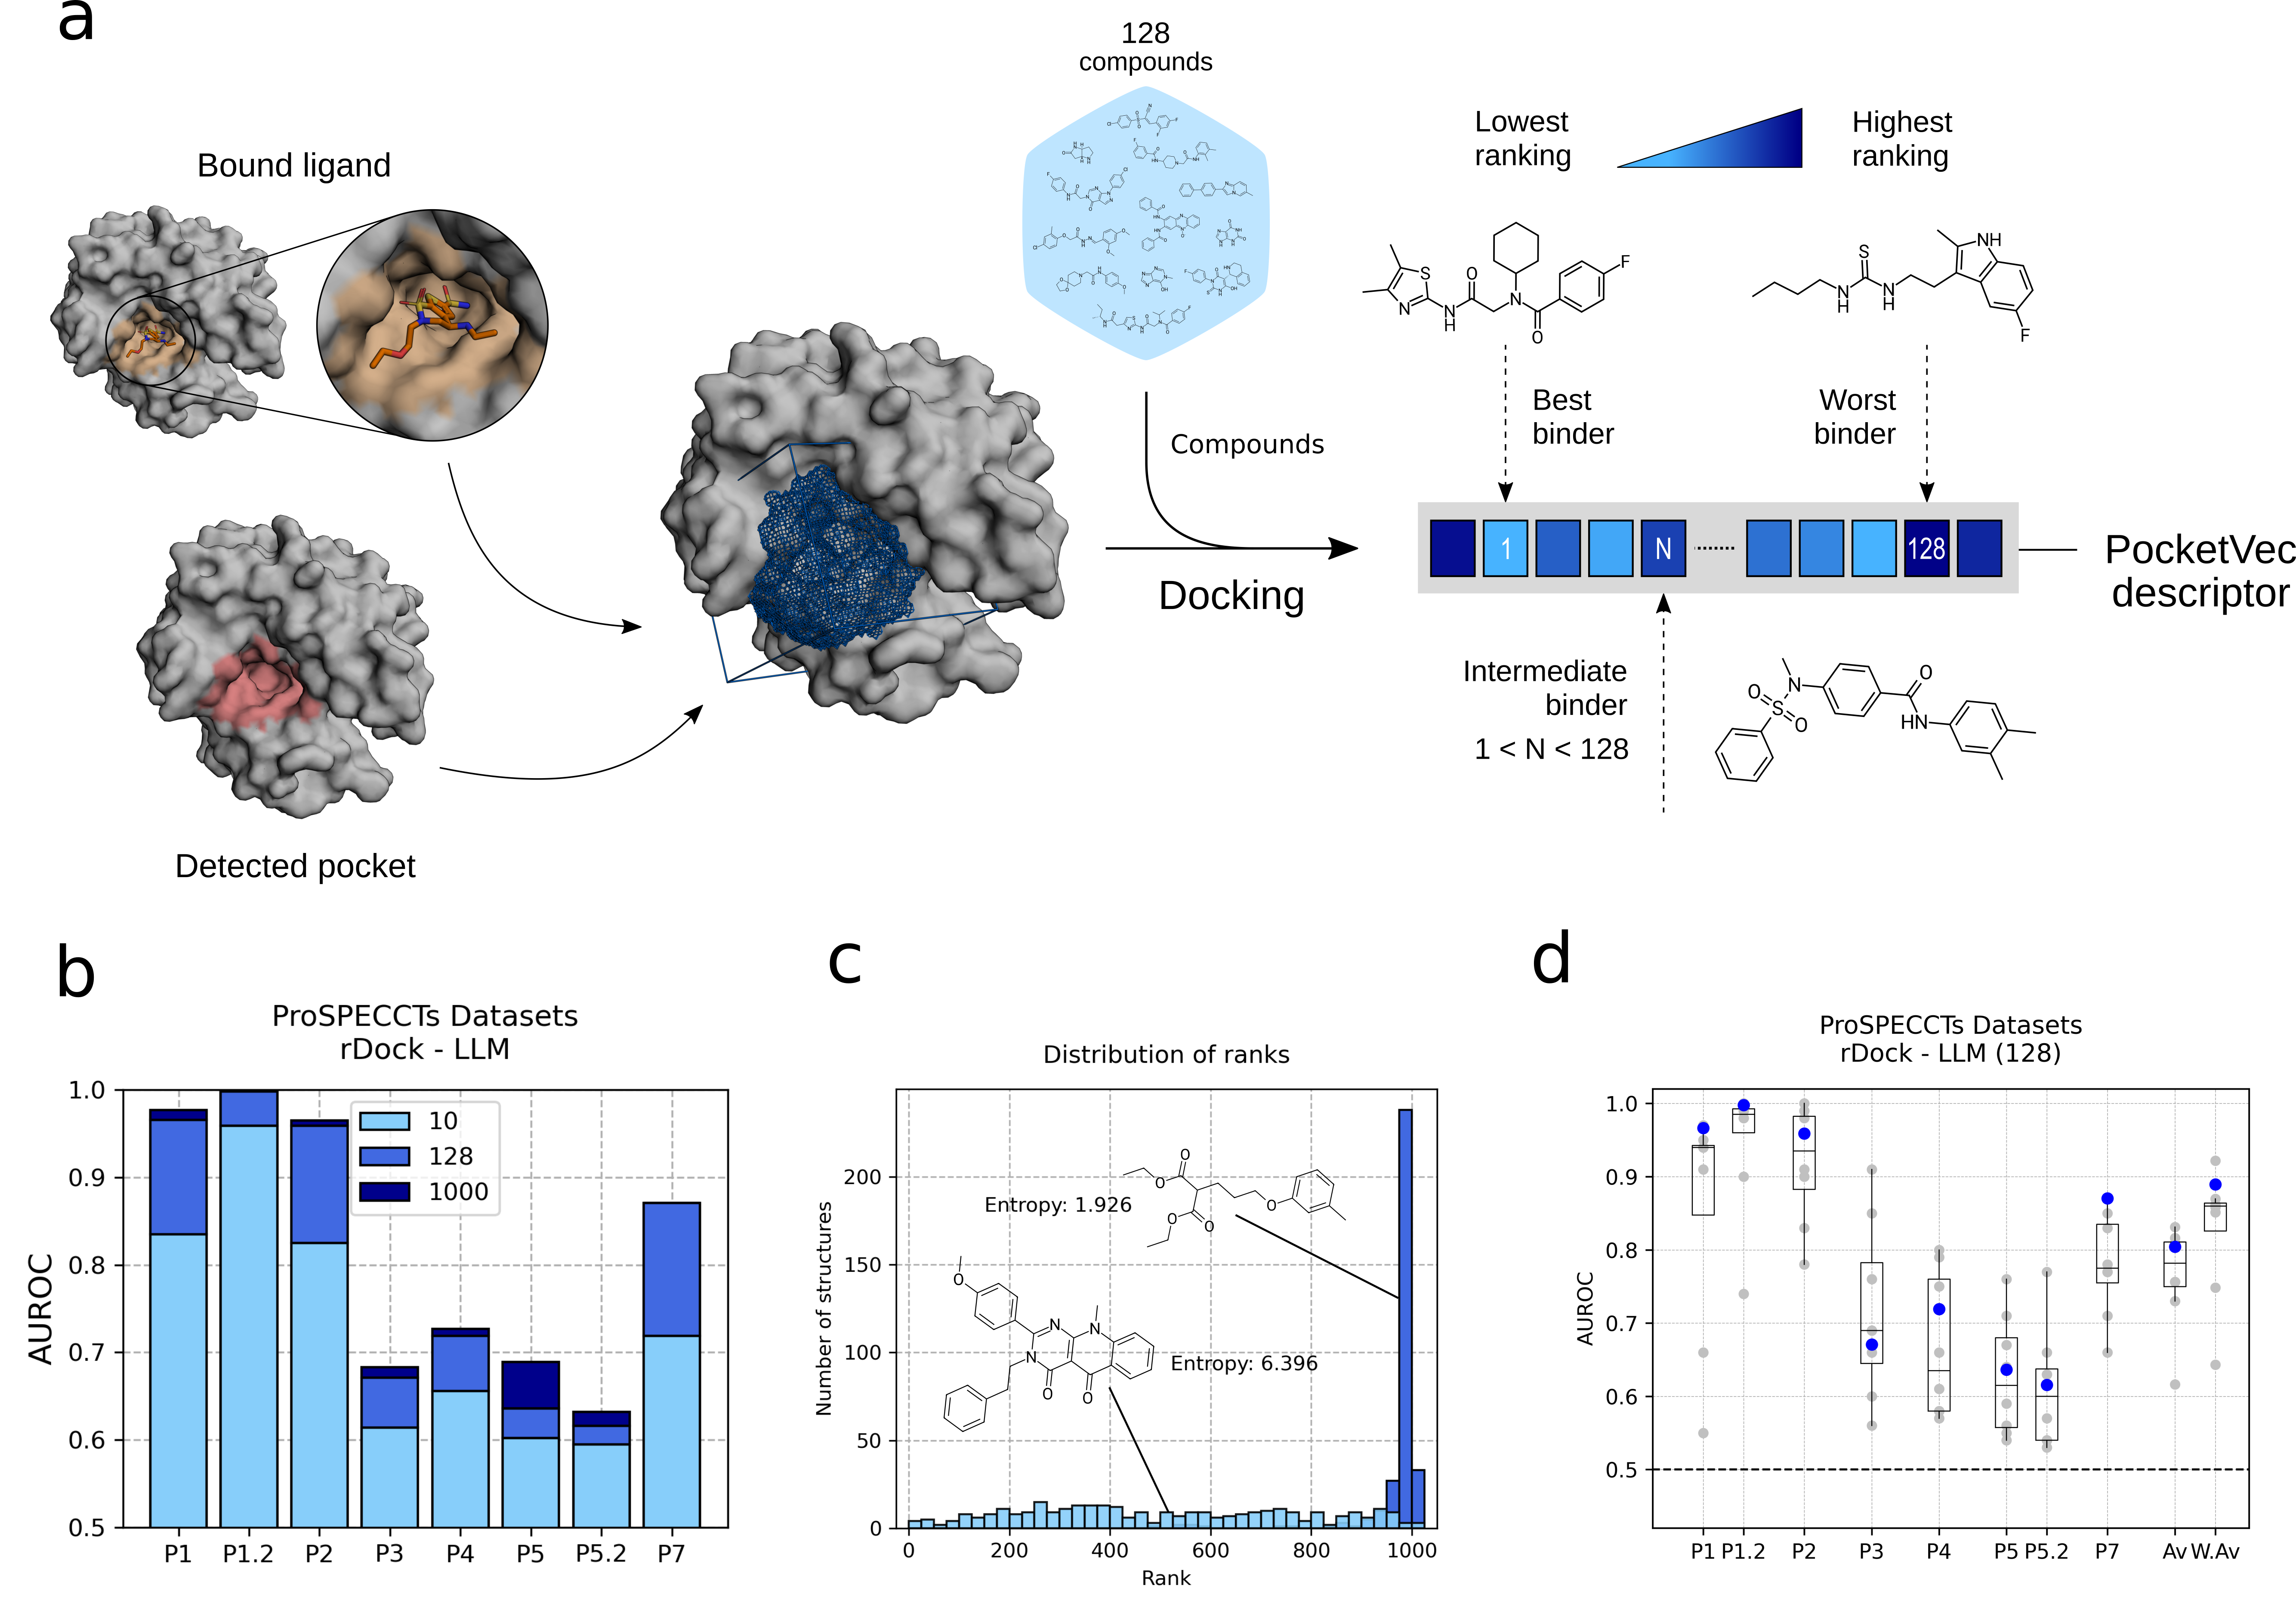
\includegraphics[width=\linewidth]{figures/PocketVec/Main/Fig1.png}
  \caption{
    \textbf{PocketVec methodological pipeline and benchmark results.} 
    \textbf{a)} Given a 3D protein structure, binding site locations are established by the presence of bound ligands or by means of pocket detection algorithms. A predefined set of compounds (128 lead-like molecules in the standard PocketVec pipeline) is docked against the pocket of interest. The corresponding docking scores are then converted into rankings and stored in a vector-type format that serves to characterize the pocket. We refer to those vectors as PocketVec descriptors.
    \textbf{b)} Bars indicating the performance (AUROC, y-axis) of our descriptors generated with a varying number of predefined molecules among ProSPECCTs datasets (x-axis, P6 and P6.2 not included. For further details, please see Online Methods). Bar color indicates the number of predefined compounds (10, 128 and the complete set of 1,000 lead-like molecules, sorted by entropy). These results correspond to the rigid docking (rDock) and LLM combination. All the other combinations with all possible numbers of predefined compounds (from 1 to complete sets) are shown in Fig \ref{PocketVec_FigS7}.
    \textbf{c)} Predefined molecules with high and low entropy. The histograms depict the distribution (y-axis) of rankings (x-axis, bin width: 25) for the highest (sky blue) and lowest (dark blue) entropy lead-like molecules in ProSPECCTs P1. Their chemical structures are shown together with the corresponding entropy values.
    \textbf{d)} Performances (AUROC, y-axis) of distinct pocket descriptors among ProSPECCTs datasets (x-axis, P6 and P6.2 not included). Gray dots represent the individual performances of existing strategies to derive pocket descriptors (see Table \ref{PocketVec_TableS1}). Box plots indicate median (middle line), 25th, 75th percentile (box), and max and min value within the 1.5*25th and 1.5*75th percentile range (whiskers). Blue dots indicate the performance of PocketVec descriptors (128 LLM and rDock rigid docking). Av. values represent the average performance among ProSPECCTs datasets for each individual method and W. Av. values weight the average value according to the number of pairs within each dataset.
  }
  \vspace{-5mm}
  \rule[0ex]{\textwidth}{0.5pt}
  \vspace{-9mm}
  \label{PocketVec_Fig1}
\end{Figure_modified}

\phantomsection
\subsubsection{PocketVec parameter selection and benchmark}

For each ProSPECCTs dataset, we generated PocketVec descriptors for all ligand-defined protein binding sites, and evaluated pocket similarity on the basis of pairwise cosine distances between PocketVec descriptors: the lower the PocketVec distance, the higher the pocket similarity. 

First, we obtained results for all possible combinations of docking strategies (rDock--rigid docking and SMINA--flexible docking) and compound collections (1,000 lead-like molecules and 667 fragments). We observed that, in general, the use of LLM and rDock rigid docking provided better results than other combinations (Fig \ref{PocketVec_FigS4}). Positive docking scores (i.e. molecules that could not be accommodated in the binding pocket, see \hyperref[PocketVec_Methods]{Methods} for further details) leading to outlier rankings were rare with fragments but more frequent when using LLM (\textasciitilde35\% of structures had at least one outlier molecule in the rDock--LLM (1,000) combination, Fig \ref{PocketVec_FigS5}). Thus, LLM showed a superior discriminative power with respect to the size of the pocket and, overall, provided higher ranking diversity among all ProSPECCTs pockets (Fig \ref{PocketVec_FigS6}). In fact, we observed how LLM occupied a larger fraction of the binding sites than fragments, while rigid docking might have removed the noise created by similar rankings of the same ligand in different conformations, overall conferring a superior discrimination capacity to the rDock--LLM combination.

Our benchmarks also revealed that some molecules were systematically ranked as very weak binders and were thus not informative for the assessment of pocket similarity. Indeed, we realized that the use of \textasciitilde100-200 molecules was often sufficient to get competitive performances in most datasets. In order to optimize the set of predefined molecules to derive pocket descriptors, we selected those LLM and fragments presenting high ranking diversity across all ProSPECCTs datasets (see \hyperref[PocketVec_Methods]{Methods}). In brief, we calculated the Shannon’s entropy for each molecule within each dataset and, after intra-dataset normalization, we assigned each molecule an averaged entropy value, which enabled us to prioritize those molecules presenting high ranking diversity (high entropy). Indeed, performances obtained in ProSPECCTs datasets by the 128 most diverse molecules were fairly similar to the original ones using complete sets of compounds (Fig \ref{PocketVec_Fig1}b, Fig \ref{PocketVec_FigS7}). Reducing the number of docked molecules (from 1,000/667 to 128) enabled a shorter length of the descriptor, now compatible with other small molecule and biological descriptors derived in the group\cite{fernandez-torras_integrating_2022, duran-frigola_extending_2020, bertoni_bioactivity_2021}, and alleviated the overall computational cost of the methodology. An illustrated example of low- and high-entropy lead-like molecules is shown in Fig \ref{PocketVec_Fig1}c.

Overall, and in view of the benchmark results, we established that the use of rigid docking (rDock) and 128 LLM was the standard and optimal methodology to generate PocketVec descriptors. All results presented along the rest of the manuscript were derived following this strategy. The selected LLM are shown in Fig \ref{PocketVec_FigS8_v2} and can also be found in our \hl{GitLab repository} in SMILES and SDF format, together with their commercial names. 



\subsection{Results and discussion}

%%%%%%%%%%%%%%%%%%%%%%%%%%%%%%%%%%%%%%%%%%%%%%%%%%%%%%%%%%%%%%%%
%%  PocketVec performance on the ProSPECCTs benchmark sets  %%%%
%%%%%%%%%%%%%%%%%%%%%%%%%%%%%%%%%%%%%%%%%%%%%%%%%%%%%%%%%%%%%%%%

\phantomsection
\subsubsection{PocketVec performance on the ProSPECCTs benchmark sets}
\label{PocketVec_ResultsAndDiscussion_PocketVec_performance_on_the_ProSPECCTs_benchmark}

The performance of PocketVec descriptors across ProSPECCTs datasets is assessed in terms of the AUROC curve and is shown in Fig \ref{PocketVec_Fig1}d. We observe that PocketVec descriptors are robust to varying definitions of the same pocket, as determined by different crystallized ligands (P1, AUROC 0.97). When restricting such definitions to chemically similar ligands, the performance is maximal (P1.2, AUROC 1.00). Similarly, our descriptors are robust against protein conformational changes, i.e. protein flexibility (P2, AUROC 0.96), and they are also able to distinguish identical pockets from those altered by 5 artificial mutations leading to changes in physicochemical and shape properties of pocket-lining residues. In these cases, we obtained more modest performances (P3--physicochemical changes and P4--both physicochemical and shape changes, AUROCs of 0.67 and 0.72, respectively). Reassuringly though, we observed a significant correlation between the number of artificial mutations (1 to 5) and the corresponding AUROC values (Pearson Corr. Coeff. > 0.98, p-value < 0.005 in both P3 and P4, Fig \ref{PocketVec_FigS9}), which confirmed that an increasing number of mutations in the binding site came along with an improved ability to detect such differences using PocketVec descriptors. 

We also benchmarked our descriptors in more biologically relevant scenarios where, for instance, pockets binding similar small molecules are found in structurally different proteins. ProSPECCTs includes two datasets to address such cases: P5 includes pocket structures classified into 9 distinct ligand classes (e.g. HEM, ATP, NAD, etc.), and P7 includes a realistic set of binding site pairs reported to be similar in published literature, some of them identified in otherwise unrelated proteins. In these sets, PocketVec descriptors show performances with AUROCs of 0.64 and 0.87, respectively, demonstrating their ability to identify similar pockets in globally dissimilar proteins. It is important to note that two binding sites having identical (or chemically similar) crystallized ligands are not necessarily similar from a PocketVec perspective. Following the logic behind the similarity ensemble approach (SEA\cite{keiser_relating_2007}), in which targets are quantitatively compared based on the chemical similarity of the ensemble of their ligands, a pair of targets sharing a single active compound may not be significantly similar.

Finally, with the goal of defining a PocketVec distance threshold to classify any pocket pair of interest as either similar or dissimilar, we analyzed the behavior of the Matthew's Correlation Coefficient (MCC) at multiple cut-off values across the different ProSPECCTs datasets (Fig \ref{PocketVec_FigS10}). As expected, each definition of pocket similarity in the ProSPECCTs datasets suggested the choice of a different cut-off distance. For instance, the optimal cut-off in the mutation-related benchmarks (P3 and P4) was around 0.13, while in the most realistic set of binding site pairs reported to be similar in published literature was even lower, around 0.08. However, for general purposes and to minimize false negatives, we selected the distance threshold based on the P1 dataset, where similar pairs were predefined as identical pockets binding chemically distinct ligands whereas dissimilar pairs were unrelated pockets binding different ligands. In this way, we defined 0.17 as our PocketVec threshold distance, which was the value maximizing the MCC in ProSPECCTs P1. However, this threshold should not be regarded as an absolute standard, but rather as a general guideline for classifying a pocket pair of interest as either similar or dissimilar.

For the sake of completeness, we generated results for all combinations of docking methods (rigid--rDock, and flexible--SMINA) and reduced sets of chemical compounds (128 LLM and 128 fragments). The use of rDock and LLM (128) was still the best strategy according to the ProSPECCTs datasets (Fig \ref{PocketVec_FigS11}). Besides, we observed that the selection of compounds leading to the most variable results throughout the different pockets (i.e. high entropy) was, indeed, of great help to distinguish similar from dissimilar pockets in ProSPECCTs P1. This effect was even more pronounced in the fragments, where their lower complexity and molecular weight led to higher promiscuity and redundancy (Fig \ref{PocketVec_FigS12}).

Detailed plots for all ProSPECCTs datasets including ROC Curves, PR Curves and distributions of PocketVec distances, docking scores and pocket volumes are included in our \href{https://gitlabsbnb.irbbarcelona.org/acomajuncosa/pocketvec}{GitLab repository} (see \hyperref[PocketVec_Code]{Code and data availability}). 



%%%%%%%%%%%%%%%%%%%%%%%%%%%%%%%%%%%%%%%%%%%%%%%%%%%%%%%%%%%%%%%%
%%%%%%%%%%  Comparison with existing strategies  %%%%%%%%%%%%%%%
%%%%%%%%%%%%%%%%%%%%%%%%%%%%%%%%%%%%%%%%%%%%%%%%%%%%%%%%%%%%%%%%

\phantomsection
\subsubsection{Comparison with existing strategies}
\label{PocketVec_ResultsAndDiscussion_Comparison_with_existing_strategies}

Next, we compared the performance of PocketVec descriptors with state-of-the-art methodologies, as reported in several studies\cite{simonovsky_deeplytough_2020, scott_classification_2022, ehrt_benchmark_2018}, where the authors benchmarked many pocket comparison tools against the ProSPECCTs datasets, including six strategies based on pocket descriptors (Fig \ref{PocketVec_Fig1}d and Fig \ref{PocketVec_FigS11}). We used the AUROC as the standard performance measure to be able to compare our results with other available methodologies. However, for PocketVec descriptors, we also provide specific values of precision, accuracy, sensitivity, specificity, Matthew´s correlation coefficient and F1 score in each ProSPECCTs dataset (Fig \ref{PocketVec_FigS13}). Overall, PocketVec is the second-best ranked strategy in terms of the weighted average among datasets (0.89, Fig \ref{PocketVec_Fig1}d) and, indeed, it surpasses the median and the average performance in all ProSPECCTs datasets, apart from P3 (Table \ref{PocketVec_TableS1}). The top-scoring method is SiteAlign\cite{schalon_simple_2008}, which is alignment-dependent and based on the projection of residue descriptors into a triangle-discretized sphere that quantifies binding site similarity by minimizing distances between systematically generated cavity fingerprints obtained by moving one binding site with respect to the other. Thus, being specifically developed to compare pockets, it does not provide a unique descriptor for each binding site, which hampers the exploration of the pocket space in the same way molecular fingerprints do for the chemical space of small molecules. Other strategies are indeed alignment-free and provide unique representations for binding sites but, apart from exhibiting worse performances than PocketVec descriptors among ProSPECCTs datasets, also present several intrinsic limitations. For instance, KRIPO\cite{wood_pharmacophore_2012} and TIFP\cite{desaphy_encoding_2013} characterize protein-ligand binding interactions between receptors and bound ligands, which enables the identification of shared interaction patterns between pockets but limits their applicability domain to \textit{holo} structures. Additionally, FuzCav\cite{weill_alignment-free_2010} fingerprints count for specific pharmacophoric triplets of pocket-lining Cα, which enables the use of \textit{apo} structures but imply a simplistic representation of pockets. On a different note, Deeplytough\cite{simonovsky_deeplytough_2020} and BindSiteS-CNN\cite{scott_classification_2022} generate pocket descriptors by means of deep learning strategies, which makes them strongly dependent on training data and provide pocket embeddings that are difficult to interpret. Thus, overall, PocketVec represents a fast strategy to generate accurate pocket descriptors that overcome the aforementioned limitations, and it shows a higher performance at assessing pocket similarities than most current strategies (Fig \ref{PocketVec_FigS14}).




%%%%%%%%%%%%%%%%%%%%%%%%%%%%%%%%%%%%%%%%%%%%%%%%%%%%%%%%%%%%%%%%
%%% Comprehensive characterization of druggable pockets in the human proteome
%%%%%%%%%%%%%%%%%%%%%%%%%%%%%%%%%%%%%%%%%%%%%%%%%%%%%%%%%%%%%%%%

\phantomsection
\subsubsection{Comprehensive characterization of druggable pockets in the human proteome}
\label{PocketVec_ResultsAndDiscussion_Comprehensive_characterization}

PocketVec descriptors constitute an optimal framework to comprehensively characterize large and diverse sets of small molecule binding sites (\textit{apo}/\textit{holo} structures), enabling the navigation across the pocket space of complete proteomes. In view of this, we designed a computational pipeline to generate PocketVec descriptors for all pockets included within human protein domains (Fig \ref{PocketVec_Fig2}a). Please, see \hyperref[PocketVec_Methods]{Methods} for a detailed description of the strategy.

%%%%%%%%%%%%%%%%
%%% FIGURE 2 %%%
%%%%%%%%%%%%%%%%


\begin{figure}[t!]
  \centering
  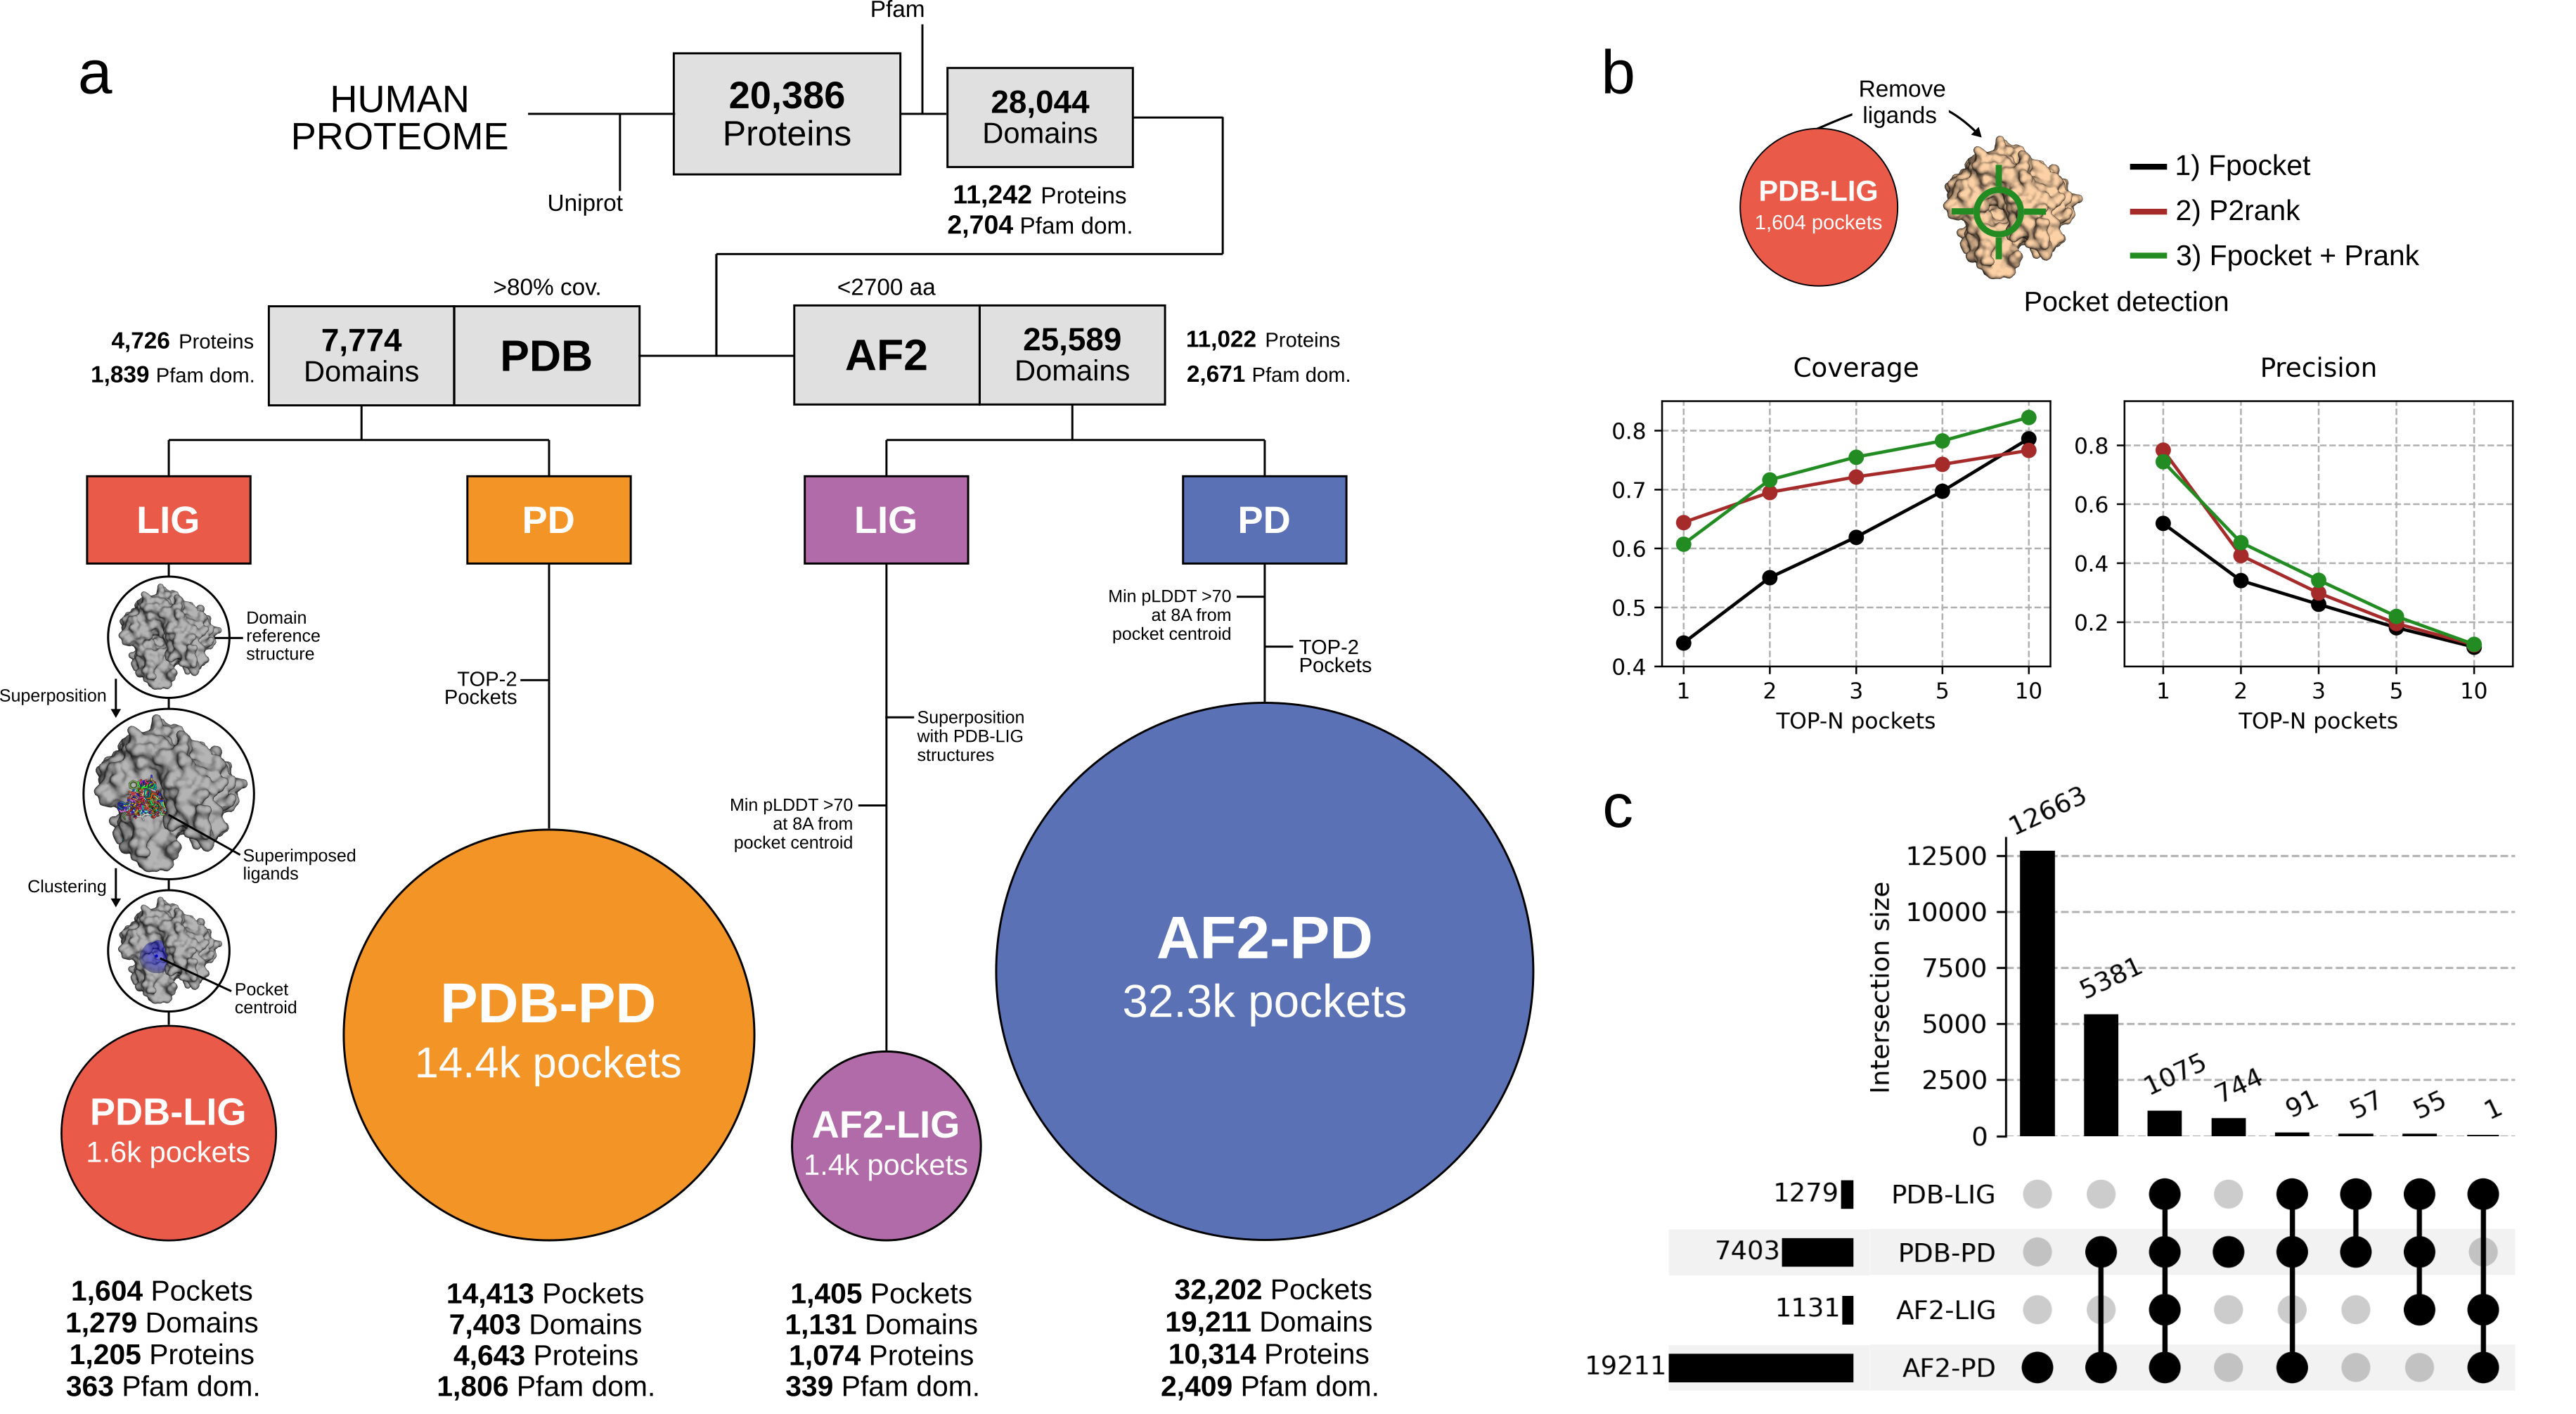
\includegraphics[width=1\linewidth]{figures/PocketVec/Main/Fig2.png} 
  \caption{
    \textbf{Generating PocketVec descriptors for all druggable pockets within human protein domains.} 
    \textbf{a)} Computational pipeline to gather all available structural data for human druggable pockets included within protein Pfam domains. Starting from the complete human proteome as per Uniprot, we first identified Pfam domains in experimentally determined structures (PDB) and AF2 predicted models. For PDB structures, we identified pockets in \textit{holo} domain structures based on the position of co-crystallized ligands (1,604 PDB-LIG pockets, red) and in \textit{apo} domain structures using pocket detection techniques (14,413 PDB-PD pockets, orange). We defined ligand-based pockets on AF2 structures (1,405 AF2-LIG pockets, purple) by directly superimposing the location of PDB-LIG pockets, and pockets were also predicted in AF2 models by means of pocket detection algorithms (32,202 AF2-PD pockets, blue).  For additional details about the pipeline, please consult the text and the \hyperref[PocketVec_Methods]{Methods} section.
    \textbf{b)} Benchmark of 3 distinct pocket detection strategies: Fpocket (black), P2rank (brown) and the combination of Fpocket and Prank (green). First, we removed bound ligands from reference PDB structures (PDB-LIG) and we then assessed the performance of the mentioned strategies to detect pockets in ligand-free structures. The plots below represent the evolution of Coverage (proportion of real pockets that are actually detected) and Precision (proportion of detected pockets that are actually real -have a crystallized ligand on PDB-LIG) in terms of the number of best-scoring detected pockets per domain that are considered (1, 2, 3, 5 and 10).
    \textbf{c)} UpSet plot representing the intersecting number of domains among pocket sets (1,279 domains in PDB-LIG, 7,403 domains in PDB-PD, 1,131 domains in AF2-LIG and 19,211 domains in AF2-PD).
  }
  \rule[0ex]{\textwidth}{0.5pt}
  \vspace{-5mm}
  
  \label{PocketVec_Fig2}
\end{figure}


In brief, we first retrieved all 20,386 human proteins in UniProt\cite{the_uniprot_consortium_uniprot_2023}. To avoid working with unstructured or very flexible regions, difficult to model and unlikely to contain druggable pockets, we only kept those protein sequences within autonomous structural units (i.e. domains), as defined in Pfam\cite{mistry_pfam_2021}. Overall, we kept 28,044 domains (2,704 unique Pfam domains) in 11,242 human proteins (Fig \ref{PocketVec_FigS15}). The next step was to structurally annotate these domains, for which we used two different strategies. On the one hand, we looked for experimentally determined structures searching the PDB\cite{goodsell_rcsb_2020}, identifying at least one PDB structure for 7,774 domains (1,839 unique Pfam domains in 4,726 proteins). Additionally, we downloaded all human predicted protein structures from AlphaFold DB, obtaining structural models for 25,589 domains (2,671 unique Pfam domains in 11,022 proteins). There is an ongoing debate on the use of AF2 models for docking experiments, and whether such models should be refined using e.g. molecular dynamics simulations. However, most studies suggest that the accuracy of AF2 models in docking experiments is comparable to experimentally determined \textit{apo} structures (i.e. without a ligand bound)\cite{zhang_benchmarking_2023, holcomb_evaluation_2023, scardino_how_2023}. Indeed, it has been recently shown that the experimental validation rates of small molecule docking are indistinguishable when PDB structures or AF2 models are used\cite{lyu_alphafold2_2023}.

Next, for each domain, we identified the potentially druggable pockets, also using two different strategies. In the first one, that we termed \textit{ligand-based} pocket definition, we searched for small molecules co-crystallized together with the protein domain, and defined druggable pockets as those having bound compounds (HET PDB codes) fulfilling the following criteria: i) being annotated as such in PDBSUM data, ii) not being one of the 20 naturally occurring amino acids, iii) having more than 6 carbon atoms, to filter out solvent molecules and crystallography-related species and iv) having solvent accessibility ≤0.4 or buriedness ≥15 (\hyperref[PocketVec_Methods]{Methods}). In total, we found at least one PDB structure containing small molecules for 1,279 domains (363 unique Pfam domains in 1,205 proteins). For 503 of these, we only found a single ligand fulfilling our criteria, whereas for 254 of them we could find 10 or more ligands (Fig \ref{PocketVec_FigS16}). Then, to compile the list of unique ligand-defined pockets, we chose a reference PDB structure for each protein domain, and superimposed all domain structures with the corresponding bound ligands onto the reference. We then used a single-linkage clustering strategy to merge into a single pocket all those ligands whose centroids were at a distance ≤5Å while maintaining the maximum distance between the global centroid of the cluster and the centroids of the individual compounds ≤18Å. We considered the final global cluster centroids as the pocket centroids. Overall, we found 1,604 ligand-defined pockets in 1,279 protein domains (363 unique Pfam domains in 1,205 proteins). We named this set of pockets \textbf{PDB-LIG}. To apply the same criteria to those structures modeled with AF2, for each domain, we superimposed the reference PDB structure onto the AF2 model, and transferred the location of the identified PDB-LIG pockets accordingly. We only considered those pockets having a pLDDT value >70 for all residues at a distance ≤8Å from the pocket centroid. In total, we identified 1,405 pockets in 1,131 domains (339 unique Pfam domains in 1,074 proteins), and named this set \textbf{AF2-LIG}. As a complementary strategy, and to increase the overall coverage of the human pocketome, we attempted a de novo identification of druggable pockets. To find the most accurate strategy to predict druggable pockets, we assessed the accuracy of different methods at identifying the PDB-LIG pockets defined above. In brief, we first removed bound ligands from reference \textit{holo} structures and used Fpocket\cite{le_guilloux_fpocket_2009} and P2rank\cite{krivak_p2rank_2018}, to detect pockets in ligand-free domain structures (\hyperref[PocketVec_Methods]{Methods}). Our benchmark showed that the best strategy to detect binding sites in ligand-free structures was the combination of Fpocket, for pocket detection, and Prank to score them. Using this combination, and considering the top-2 best scored pockets for each domain, we were able to detect 72\% of the real pockets while 47\% of detected pockets were indeed real (Fig \ref{PocketVec_Fig2}b, coverage and precision, respectively). Thus, for each domain, we ran Fpocket on the PDB reference structure to identify potential pockets, we ranked them by means of Prank, and we kept the top-2 ranked pockets per domain. Overall, this accounted for a total of 14,413 predicted pockets in 7,403 domains (1,806 unique Pfam domains in 4,643 proteins). We named this set \textbf{PDB-PD}. We then used the same strategy and criteria as before to detect pockets onto the predicted AF2 domain models, annotating a total of 32,202 pockets in 19,211 domains (2,409 unique Pfam domains in 10,314 proteins). We named this set \textbf{AF2-PD}.



%%%%%%%%%%%%%%%%%%%%%%%%%%%%%%%%%%%%%%%%%%%%%%%%%%%%%%%%%%%%%%%%
%%% Robustness in the detection of druggable pockets
%%%%%%%%%%%%%%%%%%%%%%%%%%%%%%%%%%%%%%%%%%%%%%%%%%%%%%%%%%%%%%%%

\phantomsection
\subsubsection{Robustness in the detection of druggable pockets}
\label{PocketVec_ResultsAndDiscussion_Robustness_Detection}

Globally, using the different strategies to structurally annotate human protein domains and to identify validated and potential druggable pockets, we compiled 1,604 PDB-LIG, 1,405 AF2-LIG, 14,413 PDB-PD and 32,202 AF2-PD druggable pockets, in 20,067 domains (Fig \ref{PocketVec_Fig2}a and Fig \ref{PocketVec_Fig2}c). The significant added value of \textit{de novo} methodologies is very apparent. Indeed, for 18,788 domains (93.6\%), all pockets were identified only with pocket detection strategies and, among these, 12,663 domains (63.1\%) exclusively featured pockets on AF2 models (Fig \ref{PocketVec_Fig2}c).

Interestingly, when we assessed the methodological robustness of pocket predictions using a subset of 1,000 PDB-PD domains, we observed that results slightly differed after translating and rotating structures. This effect was observed for both PDB and AF2 structures in a consistent manner: only \textasciitilde85\% and \textasciitilde86\% of detected pockets were evenly identified after rotation and translation, respectively (top-2 pockets, Fig \ref{PocketVec_FigS17}a). However, in the pockets identified regardless of variations in the initial structures, the scoring was very consistent both in PDB structures and AF2 models (Pearson CC \textasciitilde0.98). We also evaluated the coherence between pockets detected in PDB and AF2 structures, finding that only \textasciitilde59\% and \textasciitilde49\% of detected pockets were evenly identified in PDB and AF2 structures with respect to a reference PDB structure. However, as when comparing discrepancies due to different initial orientations, in the pockets identified both in PDB and AF2 structures the scoring was quite robust, with Pearson CC of \textasciitilde0.88 and \textasciitilde0.62 for PDB and AF2 models, respectively (Fig \ref{PocketVec_FigS17}b). 

Additionally, we also explored potential differences in the physicochemical properties between the real (ligand-defined) and predicted (detected) pockets, comparing their volumes and buriedness values (see \hyperref[PocketVec_Methods]{Methods}). In this case, as the only remarkable difference, we found that real pockets identified from bound ligands tended to be smaller than those predicted in the PD framework, with average volumes of \textasciitilde3,000 ų and \textasciitilde3,800 ų for LIG and PD pockets, respectively (Fig \ref{PocketVec_Fig3}a). As expected, we reached the same conclusion with buriedness values (Fig \ref{PocketVec_FigS18}), since pocket volume and buriedness were indeed negatively correlated (Fig \ref{PocketVec_FigS19}).

Altogether, these results underscore some limitations in the pocket detection strategy, revealing slight variations due to the orientation of the initial structures, a stronger dependence on structural variability and the production of predicted pockets whose physicochemical properties (e.g. volume) diverge from known pockets. 



%%%%%%%%%%%%%%%%%%%%%%%%%%%%%%%%%%%%%%%%%%%%%%%%%%%%%%%%%%%%%%%%
%%% Systematic generation of PocketVec descriptors
%%%%%%%%%%%%%%%%%%%%%%%%%%%%%%%%%%%%%%%%%%%%%%%%%%%%%%%%%%%%%%%%

\phantomsection
\subsubsection{Systematic generation of PocketVec descriptors}
\label{PocketVec_ResultsAndDiscussion_Systematic_generation_of_PocketVec_descriptors}

Once we had identified human druggable pockets with four different approaches, we systematically generated PocketVec descriptors for all of them, using the strategy described above (Fig \ref{PocketVec_Fig1}a). The high number of pockets explored enabled an exhaustive analysis of potential dependencies between the lead-like molecules used to build the descriptors and the characterization of druggable pockets. Reassuringly, we did not find any correlation between docking rankings and molecular properties of docked compounds (e.g. molecular weight or number of heavy atoms, Fig \ref{PocketVec_FigS20} and Fig \ref{PocketVec_FigS21}, respectively). On the contrary, we observed that most molecules exhibited a complete range of rankings (from 1 to 128), although the ranking distributions showed that some molecules tended to bind with good scores in many pockets while others were mostly downranked (Fig \ref{PocketVec_FigS22}). Indeed, this tendency was observed in all pocket definition strategies, and we found significant correlations between the average docking rankings for docked lead-like molecules among different pocket sets (Fig \ref{PocketVec_Fig3}b). Such correlations showed a perfect agreement between PocketVec descriptors generated through PDB and AF2 structures, but exposed slight differences between LIG and PD results (Fig \ref{PocketVec_Fig3}b, Pearson’s CC <0.88). In line with this, we found that 88.0\% and 86.8\% of the PocketVec descriptors generated for PDB-LIG and AF2-LIG, respectively, showed no lead-like molecules with positive docking scores (i.e. outlier molecules not fitting in the pocket, see \hyperref[PocketVec_Methods]{Methods}), while the fraction was considerably higher in PDB-PD and AF2-PD sets, with 97.0\% and 98.1\% of the descriptors, respectively (Fig \ref{PocketVec_Fig3}c). This result was consistent with the differences observed in pocket volumes (Fig \ref{PocketVec_Fig3}a). Reassuringly, we found that smaller pockets (<3,000ų) tended to be more prone to exhibit outlier molecules than bigger pockets (Fisher exact test, OR >70 and p-value <10\textsuperscript{-45} for all pocket sets).

%%%%%%%%%%%%%%%%
%%% FIGURE 3 %%%
%%%%%%%%%%%%%%%%

\begin{Figure_modified}
  \centering
  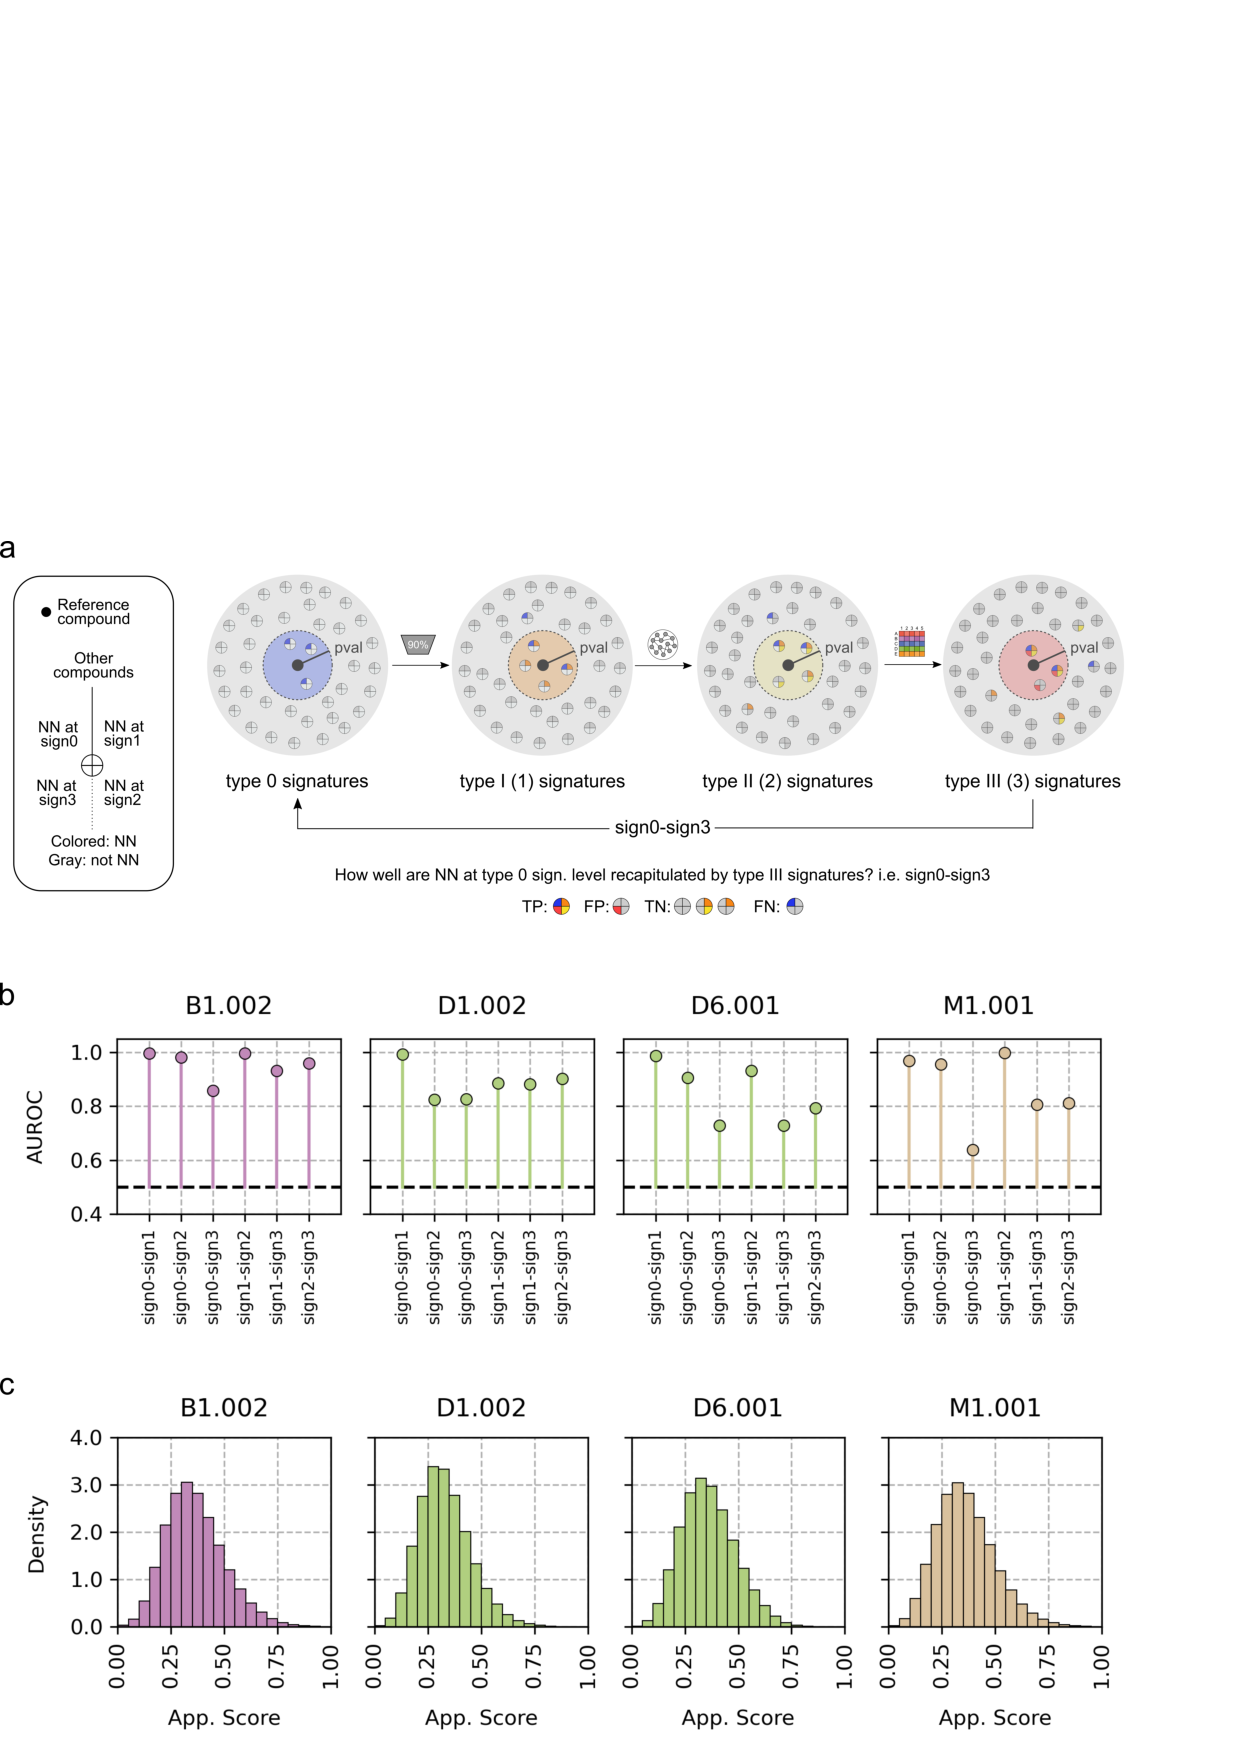
\includegraphics[width=\linewidth]{figures/PocketVec/Main/Fig3.png}
  \caption{
    \textbf{Characterization of human druggable pockets using PocketVec descriptors.} 
    \textbf{a)} Distribution of volumes (x-axis, x10³ A³) for each pocket set: PDB-LIG (1,604 pockets, red), PDB-PD (14,413 pockets, orange), AF2-LIG (1,405 pockets, purple) and AF2-PD (32,302 pockets, blue). All distributions are normalized (density, y-axis). The average volumes are 2992.88 A³, 3764.1 A³, 2940.47 A³ and 3972.66 A³, respectively. Pocket volumes were directly calculated using the rDock\cite{ruiz-carmona_rdock_2014} CAVITY functionality. 
    \textbf{b)} Correlation between average docking rankings among all pocket sets. For each pocket set, a 128-length array containing the average docking ranking for each lead-like molecule was calculated, and these arrays were compared among pocket sets by means of the Pearson’s Correlation Coefficient. All p-values (10) are <10\textsuperscript{-25}. 
    \textbf{c)} For each pocket set, proportion of PocketVec descriptors (\%, y-axis) having less than N (x-axis) outlier molecules (i.e. molecules with positive docking scores, please see \hyperref[PocketVec_Methods]{Methods}).
    \textbf{d)} Proportion of originally dissimilar pocket pairs (y-axis, distances >threshold) classified as similar (distances <threshold) due to the artificial insertion of a growing number of outlier values (x-axis) at different distance thresholds. To run the analysis, 100,000 PocketVec distances were randomly sampled (x10 times) from PDB-LIG. Solid lines represent average results and shadowed areas correspond to minimum and maximum proportions among samples. Results did not change among pocket sets (Fig \ref{PocketVec_FigS23}).
    \textbf{e)} tSNE (t-distributed Stochastic Neighbor Embedding) representation of all PocketVec descriptors within each pocket set (PDB-LIG, PDB-PD, AF2-LIG, AF2-PD). Each pocket is represented by a single point, which is colored and sized by 2D density within the pocket set. Gray dots correspond to the background space: all PocketVec descriptors are considered at once, and are also colored and sized by 2D density.
    \textbf{f)} Distributions (density, y-axis) of maximum Tanimoto Similarity among bound ligands (x-axis, bin width: 0.02) grouped by PocketVec distance ranges (0-0.10, 0.10-0.17 and 0.17-0.4). The number of pocket pairs per PocketVec distance range is specified in parenthesis.
    \textbf{g)} Distributions (density, y-axis) of PocketVec cosine distances (x-axis) grouped by the maximum Tanimoto Similarity among bound ligands (0-0.5, 0.5-0.8, 0.8-1 and 1). The number of pocket pairs per maximum Tanimoto Similarity range is specified in parenthesis.
    \textbf{h)} Distributions (density, y-axis) of PocketVec cosine distances (x-axis) grouped by the number of shared ligands between pockets (0, 1, 2 and 3 or more). The number of pocket pairs per number of shared ligands is specified in parenthesis.
  }
  \vspace{-5mm}
  \rule[0ex]{\textwidth}{0.5pt}
  \vspace{-9mm}
  \label{PocketVec_Fig3}
\end{Figure_modified}


To assess if outlier compounds could have a significant effect in the generation of poor PocketVec descriptors, we randomly inserted outlier values in the descriptors and computed the fraction of originally dissimilar pocket pairs (PocketVec distance >0.17) that were incorrectly labeled as similar (distance <0.17) due to an increasing number of outlier values. We observed that the insertion of up to 80 outlier molecules (out of 128) did not significantly compromise PocketVec descriptors, leading to only \textasciitilde0.039\% of false positives (Fig \ref{PocketVec_Fig3}d and Fig \ref{PocketVec_FigS23}). In front of this strong robustness of the descriptors, in further analyses, we only discarded those very few PocketVec descriptors with more than 80 outlier molecules (10, 45, 15 and 43 descriptors from the PDB-LIG, PDB-PD, AF2-LIG and AF2-PD sets, respectively). 



%%%%%%%%%%%%%%%%%%%%%%%%%%%%%%%%%%%%%%%%%%%%%%%%%%%%%%%%%%%%%%%%
%%% Influence of protein flexibility on PocketVec descriptors
%%%%%%%%%%%%%%%%%%%%%%%%%%%%%%%%%%%%%%%%%%%%%%%%%%%%%%%%%%%%%%%%

\phantomsection
\subsubsection{Influence of protein flexibility on PocketVec descriptors}
\label{PocketVec_ResultsAndDiscussion_Influence_of_protein_flexibility}

Proteins are dynamic entities that may adopt various 3D conformations depending on multiple environmental factors (e.g. the presence of a ligand), as well as exhibiting a certain degree of flexibility in their side chains. Indeed, a single X-ray structure often does not represent the complete structural behavior of a protein, and we thus do not expect a single PocketVec descriptor to be a global representation of a pocket but instead a snapshot for each particular structure. To some extent, the ProSPECCTs benchmark set already assesses the sensitivity of PocketVec descriptors to the binding site definition (i.e. same pocket occupied by distinct ligands, P1 and P1.2) and the impact of protein flexibility (i.e. NMR-resolved structures, P2). In this context, we observed that, as expected, the variability among PocketVec descriptors from the same pocket was lower enough to be clearly distinguished from random pairs of pockets (Fig \ref{PocketVec_Fig1}d, AUROCs of 0.97, 1.00 and 0.96 for ProSPECCTs P1, P1.2 and P2, respectively). Besides, a 2D tSNE representation of PocketVec descriptors derived from the 326 structures in P1 showed a clustering pattern consistent with the 12 pockets represented (Fig \ref{PocketVec_Fig4}a). Interestingly, we observed that one of the structures (3UAB\_B) of Poly-ADP polymerase tankyrase-2 (Q9H2K2) significantly deviated from the rest of the descriptors from the same pocket (protein) in the tSNE representation (black dots), and a visual inspection of its structure showed significant conformational changes in the side chains conforming the binding pocket with respect to the other ones (Fig \ref{PocketVec_Fig4}b), which translated into a higher PocketVec distance (>0.17) with the rest of the descriptors of the same pocket. In any case and, as briefly mentioned above, PocketVec descriptors for holo structures of the same pocket (ProSSPECTs P1 similar pairs) were fairly similar, with almost 80\% of the pairs showing distances <0.17, while only 1,2\% of the pairs showed distances <0.17 for dissimilar pocket pairs. When comparing holo structures to the corresponding apo structures or AF2 models of the same pocket, we found that the PocketVec descriptors showed higher variability than within \textit{holo} structures, reflecting pocket structural heterogeneity (Fig \ref{PocketVec_FigS24}). However, the distributions of distances comparing \textit{holo} with \textbf{apo} or AF2 structures were very similar, with 51\% and 55\% of pairs pairs below the 0.17 threshold, respectively. To further complement this result, we performed an exhaustive evaluation of the behavior of PocketVec descriptors upon protein flexibility and conformational changes. In short, we kept those pockets from the PDB-LIG set for which we had enough \textit{holo} and \textit{apo} PDB structures available (≥10, see \hyperref[PocketVec_Methods]{Methods}) as well as a confident AF2 model, and generated PocketVec descriptors for all their structures. Overall, we collected 903 PocketVec descriptors corresponding to 43 unique pockets (10 holo structures, 10 apo structures and 1 AF2 model each). We then computed PocketVec distances between same-pocket holo PDB structures (LIG-LIG), same-pocket holo and apo PDB structures (LIG-PD), same-pocket apo PDB structures (PD-PD), same-pocket holo PDB and AF2 structures (LIG-AF2) and, finally, same-pocket apo PDB and AF2 structures (PD-AF2). Additionally, we compared holo (PDB), apo (PDB) and AF2 structures against our 4 sets of precompiled PocketVec descriptors (i.e. PDB-LIG, PDB-PD, AF2-LIG and AF2-PD) in order to contextualize the results with background distance distributions (Fig \ref{PocketVec_Fig4}c). We observed that PocketVec descriptors derived from holo PDB structures were rather robust and clearly distinguishable from random pocket pairs (LIG-LIG, AUROC of 0.90 against background distance distributions), in perfect agreement with the results obtained in ProSPECCTs P1 and P1.2. When we compared descriptors derived from holo and apo PDB structures, as expected, the intrinsic and increased variability of ligand-free structures was reflected in the PocketVec distances, which affected the ability to recapitulate pocket structures from the same protein (LIG-PD, AUROC of 0.77; PD-PD, AUROC of 0.80). Finally, we also observed that descriptors derived from holo structures tended to be more similar to those derived from AF2 models than to those from apo PDB structures (LIG-AF2, AUROC of 0.82). This observation aligns with several studies stating that AF2-predicted structures are comparable to the apo conformations and, perhaps, a bit closer to the holo conformations due to the nature of the training data (which includes both holo and apo structures)\cite{zhang_benchmarking_2023}.


Additionally, we sampled MD trajectories for 192 pockets from the PDB-LIG and PDB-PD sets, considering 10 conformations per pocket, and then, for each pocket, we calculated all pairwise distances among their PocketVec descriptors (see Online Methods). As in the previous exercise, we also compared the obtained PocketVec descriptors with a random sample of precomputed descriptors from the PDB-LIG, PDB-PD, AF2-LIG and AF2-PD sets (Fig \ref{PocketVec_Fig4}d). Overall, we observed a similar trend than when comparing \textit{apo} PDB structures: PocketVec descriptors showed variations responding to the flexibility of the proteins, while still recognizing different conformations from the same pocket (AUROC of 0.78). Finally, we analyzed the correlation between PocketVec distance among MD frames and the all-atom RMSD (excluding hydrogen atoms) considering both complete structures and only pocket residues (at <8Å from the pocket centroid in any of the MD used frames). We found a weak correlation (Fig \ref{PocketVec_Fig4}e; Pearson CC 0.39) with the full structure RMSD that increased (Fig \ref{PocketVec_Fig4}f; Pearson CC 0.49) when exclusively considering pocket residues. 

The presence of metal atoms is often required for many pockets to perform its native function (e.g. to act as catalytic centers or to stabilize protein structures). However, our study does not explicitly consider the presence of other compounds such as cofactors or metal atoms which, despite the limitations, it enables a fair and analogous characterization with different protein structures and pocket identification strategies where bound metal atoms are not available (e.g. PDB vs AF2 or LIG vs PD). Thus, finally, we also assessed the ability of our precomputed PocketVec descriptors to identify pocket similarities among metal-binding proteins. For this, after collecting all PDB-LIG and PDB-PD pockets with bound metal atoms, we compared the derived PocketVec descriptors with and without the metal atoms (\hyperref[PocketVec_Methods]{Methods}). We observed that, although descriptors were obviously not identical, the vast majority of the identified metal-binding pockets had similar PocketVec descriptors with and without the explicit presence of the metal atoms (Mann-Whitney p-value <10\textsuperscript{-100}; Fig \ref{PocketVec_FigS25}). 

Overall, these results illustrate the capacity of PocketVec descriptors to capture pocket flexibility and protein conformational changes, revealing their sensitivity to changes in the pocket shapes as well as their feasibility of use with \textit{holo} and \textit{apo} PDB structures (including metal-binding proteins) and AF2 predicted models. 


%%%%%%%%%%%%%%%%
%%% FIGURE 4 %%%
%%%%%%%%%%%%%%%%


\begin{Figure_modified}
  \centering
  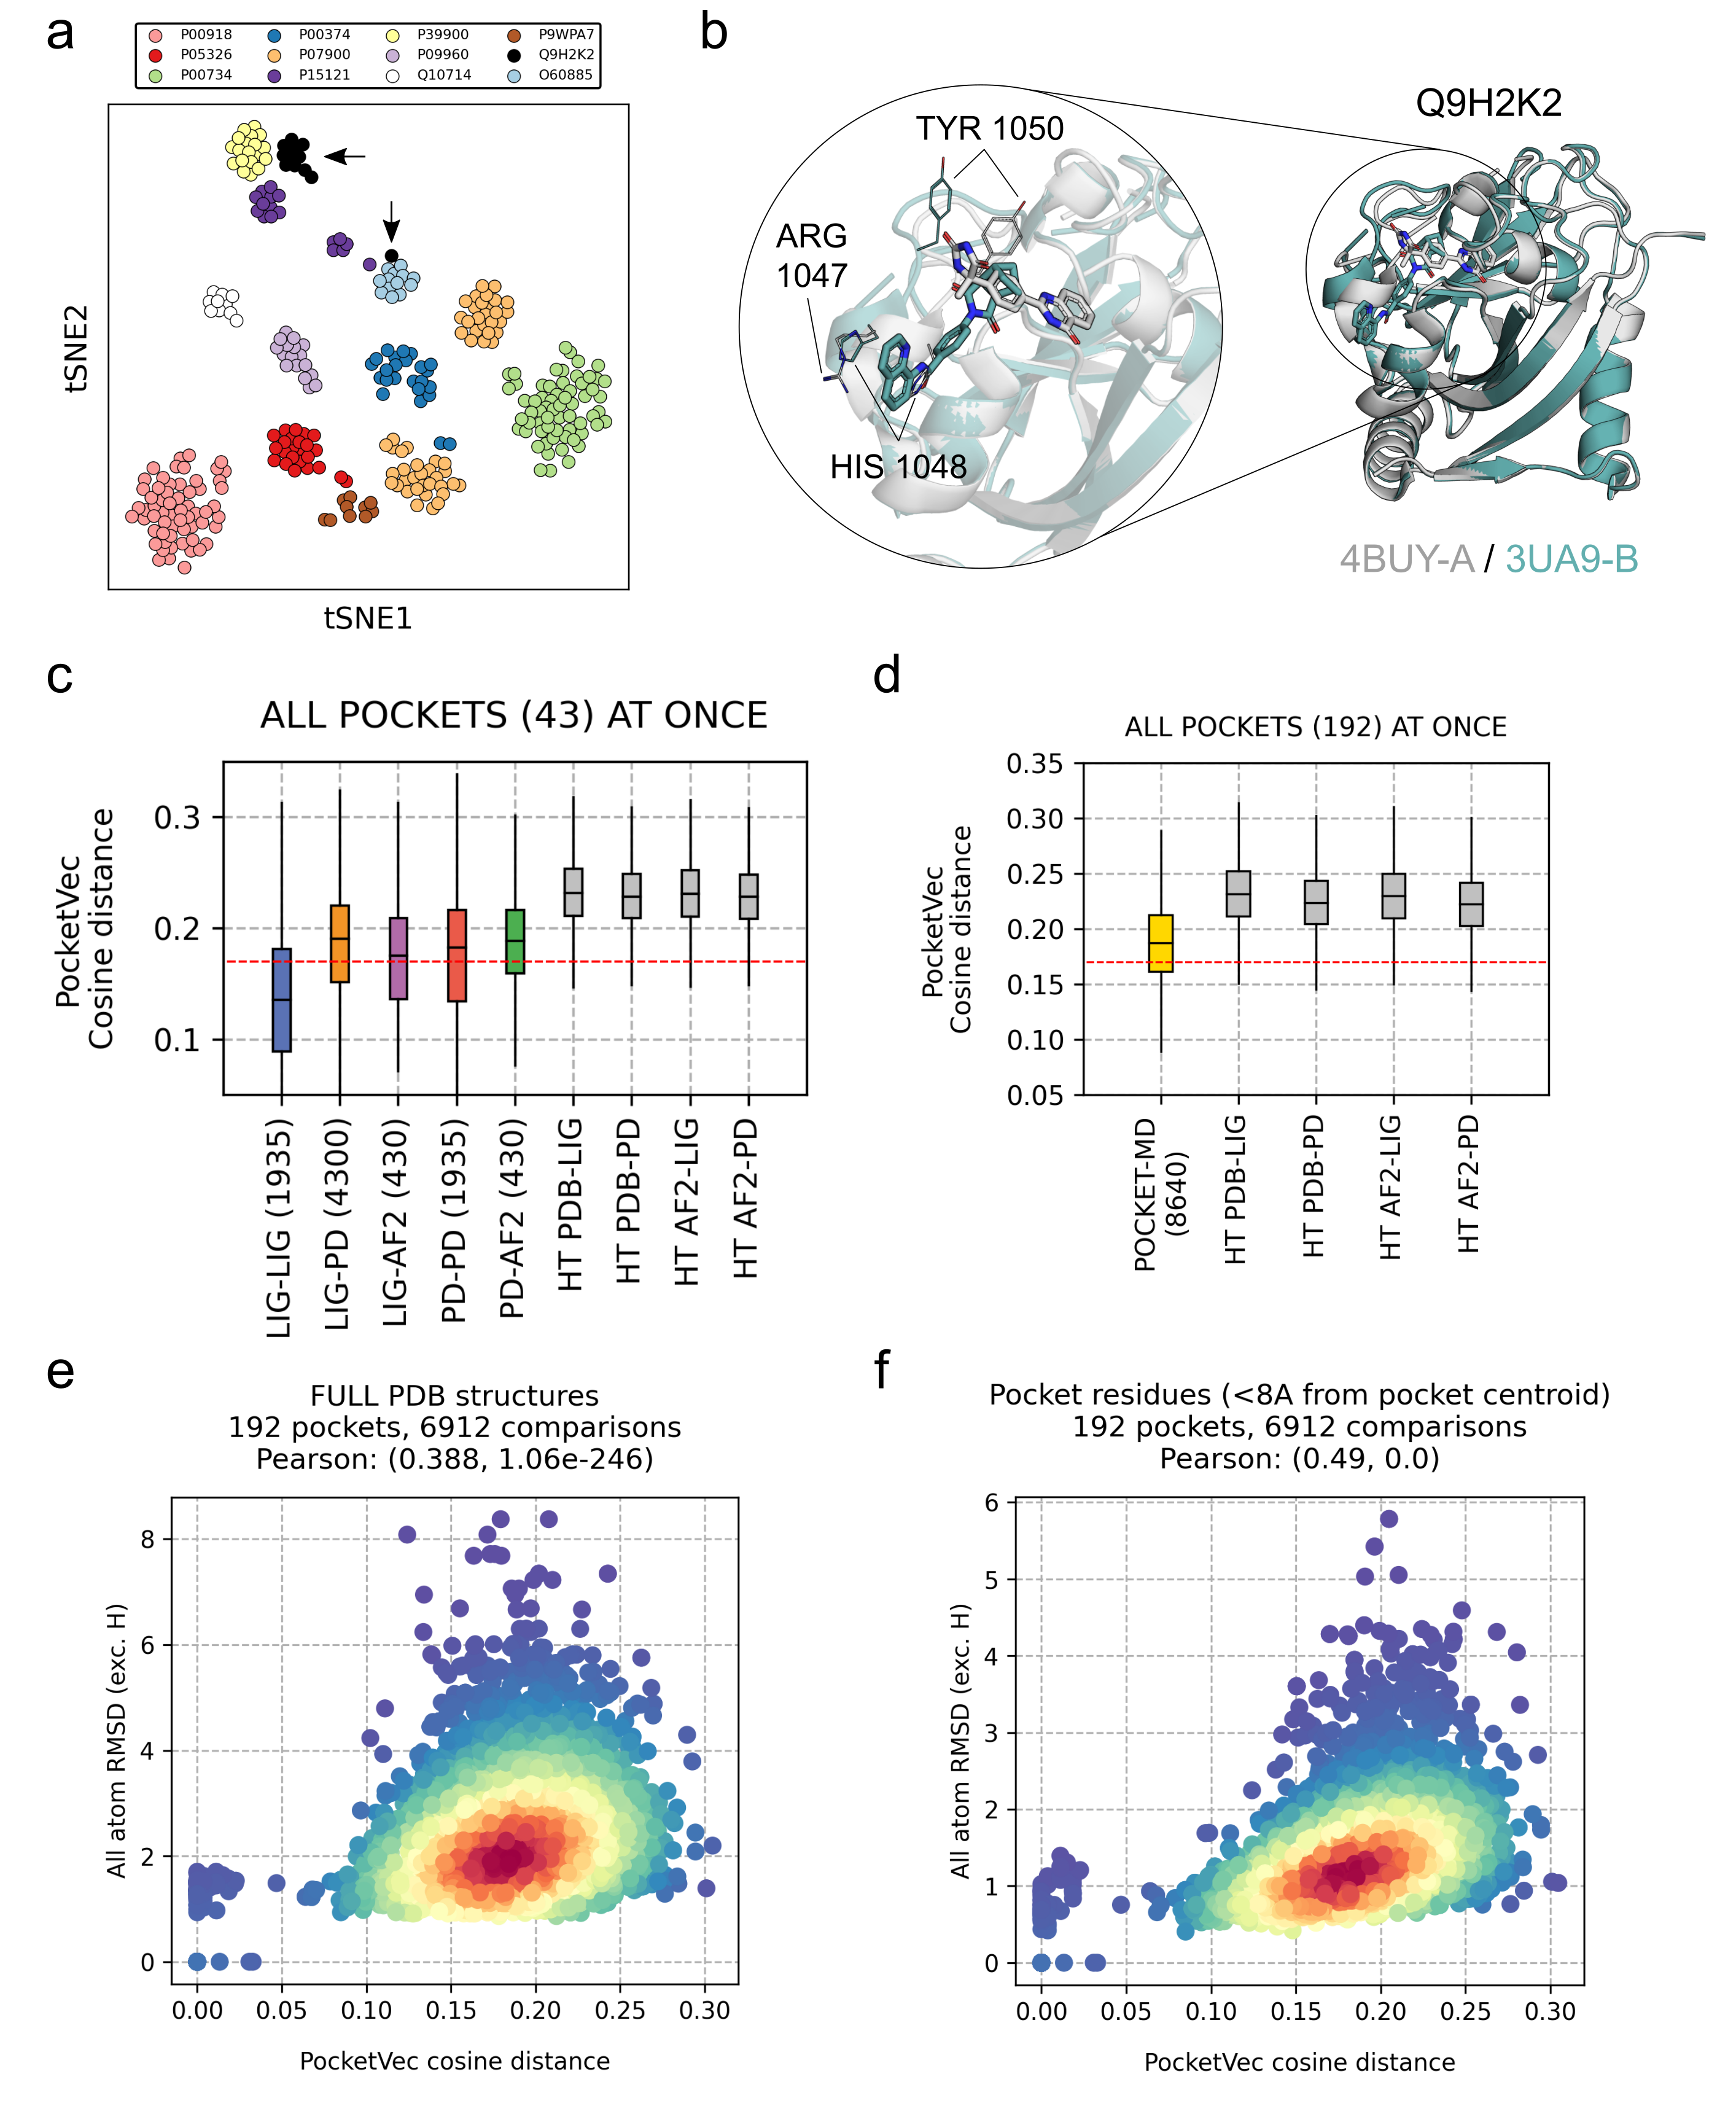
\includegraphics[width=\linewidth]{figures/PocketVec/Main/Fig4.png} 
  \caption{
    \textbf{Assessment of the effect of protein flexibility.} 
    \textbf{a)} 2D tSNE representation of 326 PocketVec descriptors representing the conformational ensemble of 12 pockets binding distinct ligands (ProSPECCTs P1). Black arrows indicate the Poly-ADP polymerase tankyrase-2 (Q9H2K2) structures.
    \textbf{b)} Structural superimposition of 4BUY\_A (white) against 3UA9\_B (teal) performed with TM-align\cite{zhang_tm-align_2005}.
    \textbf{c)} PocketVec descriptors’ variability caused by protein flexibility and conformational changes. Each boxplot indicates the distribution of PocketVec distances of the same pocket in i) holo PDB structures (LIG-LIG), ii) holo and apo PDB structures (LIG-PD), iii) holo PDB and AF2 structures (LIG-AF2), iv) apo PDB structures (PD-PD), v) apo PDB and AF2 structures (PD-AF2) and holo (LIG), apo (PD) and AF2 structures (AF2) against each of the 4 sets of PocketVec descriptors from our study (i.e. PDB-LIG, PDB-PD, AF2-LIG, AF2-PD). Boxplots indicate median (middle line), 25th, 75th percentile (box), and max and min value within the 1.5*25th and 1.5*75th percentile range (whiskers).
    \textbf{d)} PocketVec descriptors’ variability caused by protein flexibility and conformational changes among MD-derived structures. POCKET-MD represents the distances between same-pocket MD-derived PocketVec descriptors and all the other boxplots represent the distances between such MD-derived descriptors and each of the 4 sets already precomputed (i.e. PDB-LIG, PDB-PD, AF2-LIG, AF2-PD).
    \textbf{e)} Correlation between PocketVec cosine distance (x-axis) and all-atom (excluding hydrogens) RMSD for the full PDB structure and
    \textbf{f)} pocket residues only. The study involved 192 pockets (8 from PDB-LIG and 184 from PDB-PD) with MD-simulation data (3 frames per replica, 3 replicas). Both plots are colored by density (the redder the higher).
  }
  \vspace{-5mm}
  \rule[0ex]{\textwidth}{0.5pt}
  \vspace{-9mm}
  \label{PocketVec_Fig4}
\end{Figure_modified}


%%%%%%%%%%%%%%%%%%%%%%%%%%%%%%%%%%%%%%%%%%%%%%%%%%%%%%%%%%%%%%%%
%%% All-vs-all comparison of human druggable pockets
%%%%%%%%%%%%%%%%%%%%%%%%%%%%%%%%%%%%%%%%%%%%%%%%%%%%%%%%%%%%%%%%

\phantomsection
\subsubsection{All-vs-all comparison of human druggable pockets}
\label{PocketVec_ResultsAndDiscussion_All_vs_All_comparison_human_druggable_pockets}

The vector-like nature of PocketVec descriptors makes them perfectly suited for extremely fast comparisons by computing simple cosine distances, enabling comprehensive proteome-wide similarity searches. We first generated a t-distributed Stochastic Neighbor Embedding (t-SNE) representation for all PocketVec descriptors to facilitate a qualitative visualization of the characterized pocket space (Fig \ref{PocketVec_Fig3}e). This visualization underlined several interesting points, some of which have already been discussed in previous sections: (i) pockets defined by bound ligands (PDB-LIG and AF2-LIG) predominantly occupy well defined regions of the pocket space, (ii) pocket detection strategies (PDB-PD and AF2-PD) significantly contribute to expand the overall coverage of the human druggable pocket space, (iii) the use of AF2 models particularly bolsters this expansion. Perhaps more interestingly, the PDB-PD and AF2-PD maps highlight dense areas of the human pocket space for which we do not yet have any experimental structure with a bound chemical compound.

Then, we systematically evaluated the validity of the chemogenomic hypothesis behind the generation of PocketVec descriptors (i.e. similar pockets bind similar ligands). We compared all PDB-LIG pockets having PocketVec descriptors (1,594 pockets, \textasciitilde1.27M comparisons) on the basis of the maximum Tanimoto similarity among their bound ligands using ECFPs (2,048 bits and radius 2), and we grouped pocket pairs according to their cosine PocketVec distance (Fig \ref{PocketVec_Fig3}f). We found that, indeed, pocket pairs with small PocketVec distances (<0.10) typically showed higher maximum Tanimoto similarities (>0.85) among their ligands than pocket pairs with high PocketVec distance (>0.17, Fisher’s exact test OR >90 and p-value <10\textsuperscript{-300}), thus supporting our underlying hypothesis. However, the fact that similar pockets bind similar ligands does not necessarily imply that similar ligands bind similar pockets. Indeed, we observed that, in general, PocketVec distances did not decrease substantially when increasing the maximum Tanimoto similarity among bound ligands (Fig \ref{PocketVec_Fig3}g). The only exception was for almost identical ligands (Tanimoto similarities=1), which showed a very subtle deviation towards smaller PocketVec distances (AUROC 0.59, true positives having Max. Tanimoto Similarity=1, true negatives having Max. Tanimoto Similarity in the [0, 0.5) range), in line with the behavior observed in ProSPECCTs P5 (AUROC=0.64) and P5.2 (AUROC=0.62). While this may seem somewhat counterintuitive, it serves as evidence to decipher the quantification of pocket similarity using PocketVec descriptors. 

The fact that a single compound is consistently upranked for two pockets may indeed be a first evidence of pocket similarity but falls short to provide similar PocketVec descriptors if no other compound is ranked in a systematic manner. In practical terms, this translates into pockets that share a growing number of ligands being more likely to be similar from a PocketVec perspective, as highlighted by Shoichet and co-workers when they presented their similarity ensemble approach (SEA) to unveil protein remote relationships\cite{keiser_relating_2007}. Reassuringly, we found that pockets that shared ligands in the PDB-LIG set tended to be more similar (i.e. smaller PocketVec distances) than pockets sharing no ligands (Fig \ref{PocketVec_Fig3}h). However, the deviation towards smaller distances for pockets sharing a single ligand was subtle (AUROC = 0.58, true positives sharing 1 ligand and true negatives sharing no ligands), but when 3 or more ligands were shared between pockets, the effect was already notable (AUROC = 0.75, true positives sharing 3 or more ligands and true negatives sharing no ligands). We also found that only 2.1\% of pocket pairs sharing no ligands in the PDB-LIG set showed PocketVec distances <0.17, while this fraction increased to 26.1\% when 3 or more ligands were shared between pockets. However, it is obvious that the lack of shared co-crystallized compounds between two pockets does not necessarily mean that they might not have common ligands. To overcome the limitation of potentially missing ligands, we used a pure computational strategy: we computed docking scores for the 128 standard lead-like molecules (see \hyperref[PocketVec_MethDevAndImp]{Methodological development and implementation}) against all PDB-LIG defined pockets and labeled them as active (the top 1\% of docking scores) or inactive (Fig \ref{PocketVec_FigS26}a). We observed that the vast majority of the lead-like molecules (127 out of 128) were cataloged as active in, at least, one pocket (Fig \ref{PocketVec_FigS26}b), and almost 20,000 of the potential \textasciitilde1,29M PDB-LIG pocket pairs shared, at least, one active lead-like molecule (Fig \ref{PocketVec_FigS26}c). With this alternative approach, we confirmed the tendency observed using experimental data: the more shared ligands between pockets, the smaller their PocketVec distance (AUROC = 0.87 when comparing pockets sharing no ligands and those sharing 3 or more ligands; Fig \ref{PocketVec_FigS26}d).

Next, we explored the complementarity and added value of PocketVec descriptors with respect to more established strategies to compare protein families and druggable pockets, such as sequence and structure similarity. First, we sought to investigate the correlation between sequence, structure and PocketVec similarity (defined as 1-PocketVec distance) among pockets located in the same Pfam domains in the more comprehensive set of AF2-PD pockets (see \hyperref[PocketVec_Methods]{Methods}). As expected, we found that the higher the sequential and structural similarity between compared pockets (assessed by sequence identity and Cα RMSD, respectively), the more similar they were according to PocketVec descriptors (Pearson CC of 0.55 and -0.35, respectively, p-value<10\textsuperscript{-100} in both cases; Fig \ref{PocketVec_Fig5}a). Reassuringly, the observed correlations were also found when computed on AF2-LIG pockets (Pearson CC of 0.57 and -0.35 for sequence identity and Cα RMSD, respectively Fig \ref{PocketVec_FigS27}). However, there were indeed cases where the results did not align perfectly, underscoring the distinctive and complementary insights that PocketVec descriptors can provide beyond traditional sequential and structural analyses.

Additionally, we also ran an all-against-all pocket comparison within and across pocket sets (PDB-LIG, PDB-PD, AF2-LIG and AF2-PD), computing over 1.2 billion pocket comparisons. Interestingly, we found more than 3.5 million similar pockets in domains having low sequential and structural similarities (PocketVec distance <0.17; TM-score <0.35; Sequence identity <30\%). For instance, we found similar pockets (PocketVec distance: 0.14, both pockets in the PDB-LIG set) in the CPSase\_L\_D2 ATP-binding domain (PF02786) of the Carbamoyl-phosphate synthase (P31327, positions 1088-1291) and in the NDK domain of the Nucleoside diphosphate kinase 3 (Q13232, positions 22-156), although they shared a sequence identity of only 28\% and a poor structural similarity (TM-score=0.31, RMSD=4.3Å). Reassuringly, crystal structures confirmed that both pockets can bind ADP (PDB IDs: 5DOU and 1ZS6, respectively), which strengthened our observation that these pockets were indeed similar (Fig \ref{PocketVec_Fig5}b). The inventory of all similar pockets (PocketVec distance <0.17) together with structural and sequential comparisons at domain level are reported in our \hl{GitLab}. On the other hand, our analyses also revealed more than 29k pocket pairs (out of a subsample of 11.1 million pairs having PocketVec distance >0.20) that, despite being similar in terms of sequence and structure, showed quite dissimilar pockets (PocketVec distance >0.20; TM-score >0.50; Sequence identity >40\%). As an illustrative example, we identified different druggable pockets (PocketVec distance: 0.21, both pockets in the AF2-PD set) in the NIPSNAP domain (PF07978) of the Protein NipSnap homolog 3B (Q9BS92, positions 146-245) and in the NIPSNAP domain (PF07978) of the Protein NipSnap homolog 3A (Q9UFN0, positions 146-245), although these domains had a sequence identity of 93\% and also a very high level of structural similarity (Fig \ref{PocketVec_Fig5}c, TM-score=0.98 and RMSD=0.4Å).

%%%%%%%%%%%%%%%%
%%% FIGURE 5 %%%
%%%%%%%%%%%%%%%%

\begin{Figure_modified}
  \centering
  \includegraphics[width=\linewidth]{figures/PocketVec/Main/Fig5.png} 
  \caption{
    \textbf{Using PocketVec descriptors to assess proteome-wide pocket similarity: achieving otherwise unattainable insights.} 
    \textbf{a)} Correlation between PocketVec similarity (x-axis, defined as 1-PocketVec distance), structural similarity (y-axis, Cα RMSD) and sequence identity (color) among pockets located at the same Pfam domains (max. 10) in the AF2-PD pocket set. Pearson CC between PocketVec similarity and sequence identity: 0.55 (p-value\textasciitilde0). Pearson CC between PocketVec similarity and RMSD: -0.35 (p-value\textasciitilde0).
    \textbf{b)} Similar pockets found in dissimilar domains. Pockets were found in the CPSase\_L\_D2 ATP-binding domain (PF02786, top structure, wheat color) of the Carbamoyl-phosphate synthase (P31327, positions 1088-1291. PDB ID: 5DOU) and in the NDK domain (PF00334, bottom structure, pale green color) of the Nucleoside diphosphate kinase 3 (Q13232, positions 22-156. PDB ID: 1ZS6). Pockets (both in the PDB-LIG set) have a PocketVec distance of 0.14 (below the established threshold of 0.17, please see \hyperref[PocketVec_ResultsAndDiscussion_PocketVec_performance_on_the_ProSPECCTs_benchmark]{PocketVec performance on the ProSPECCTs benchmark sets}) although domains share a sequence identity of only 28\% and a poor structural similarity (TM-score=0.31, RMSD=4.3Å).
    \textbf{c)} Dissimilar pockets found in similar domains. Pockets were found in the NIPSNAP domain (PF07978) of the Protein NipSnap homolog 3B (Q9BS92, positions 146-245, AF2 model, pink residues) and in the NIPSNAP domain (PF07978) of the Protein NipSnap homolog 3A (Q9UFN0, positions 146-245, AF2 model, green residues). The former is used as the reference structure (gray cartoon). Pockets (both in the AF2-PD set) have a PocketVec distance of 0.21 (above the established threshold of 0.17, please see \hyperref[PocketVec_ResultsAndDiscussion_PocketVec_performance_on_the_ProSPECCTs_benchmark]{PocketVec performance on the ProSPECCTs benchmark sets}) although domains have a sequence identity of 93\% and also a very high level of structural similarity (TM-score=0.98 and RMSD=0.4Å).
  }
  \vspace{-5mm}
  \rule[0ex]{\textwidth}{0.5pt}
  \vspace{-9mm}
  \label{PocketVec_Fig5}
\end{Figure_modified}




%%%%%%%%%%%%%%%%%%%%%%%%%%%%%%%%%%%%%%%%%%%%%%%%%%%%%%%%%%%%%%%%
%%% Relationship between PocketVec similarity and experimentally determined compound-target pairs
%%%%%%%%%%%%%%%%%%%%%%%%%%%%%%%%%%%%%%%%%%%%%%%%%%%%%%%%%%%%%%%%

\phantomsection
\subsubsection{Relationship between PocketVec similarity and experimentally determined compound-target pairs}
\label{PocketVec_ResultsAndDiscussion_Relationship_PocketVecSimilarity_CPD-TARGET_pairs}

To further validate the ability of PocketVec descriptors to identify similar protein binding pockets, we explored the relationship between pocket similarity and experimentally determined compound-target pairs by assessing the number of shared compounds between proteins with different degrees of pocket similarity. We processed data on 836,654 compounds bound to 6,933 protein targets from ChEMBL\cite{zdrazil_chembl_2024} and BindingDB\cite{gilson_bindingdb_2016}, and we also collected all PocketVec descriptors from our study (i.e. PDB-LIG, PDB-PD; AF2-LIG and AF2-PD) and kept only those protein pairs for which there was, at least, one reported bound small molecule per protein (\hyperref[PocketVec_Methods]{Methods}). Overall, we evaluated 2,055,378 protein pairs on the bases of the number of shared compounds and the cosine distances between their PocketVec descriptors. Note that, since the experimental data reported compound-target pairs, without information on specific pockets, we always took the minimal PocketVec distance between each pair of proteins (i.e. the most similar pockets). 

We first calculated the number of protein pairs within each range of PocketVec distances in an all-vs-all comparison of PocketVec descriptors, regardless of their set of origin (e.g. PDB-LIG, AF2-PD, etc) (Fig \ref{PocketVec_Fig6}a). Then, we checked the distribution of shared compounds between each protein pair plotted against their minimal PocketVec distance. We observed that, the lower the minimal PocketVec distance between two proteins, the higher the number of compounds binding them both and, for PocketVec distances ≥0.2, there were almost no shared compounds for any protein pair (Fig \ref{PocketVec_Fig6}b). Further, we calculated the odds ratio considering a varying number of shared compounds for PocketVec distances ≤0.17, ≤0.10 and ≤0.05. We found that, indeed, there was a clear enrichment of protein pairs sharing compounds among protein pairs with similar pockets. (Fig \ref{PocketVec_Fig6}c). For instance, we found \textasciitilde2, \textasciitilde50 and \textasciitilde200 fold enrichments of protein pairs sharing ≥5 compounds in protein pairs with minimal PocketVec cosine distances below 0.17, 0.10 and 0.05, respectively. And these enrichments went up to \textasciitilde5, \textasciitilde300 and \textasciitilde700 if we considered protein pairs sharing ≥20 compounds. Finally, to overcome potential biases due to the comparison of PocketVec descriptors from the same origin (e.g. PDB-LIG, AF2-PD, etc), we repeated the analysis considering only comparisons between the PDB-LIG set (i.e. derived from experimental structures with co-crystallized compounds) and the other sets, observing a very similar result (Fig \ref{PocketVec_FigS28}a, b, c).

Additionally, we checked the robustness of our results on a novel dataset where Winter and co-workers comprehensively tested the potential binding of 407 fragment compounds on 5,951 proteins. After applying the filtering criteria to the raw data defined by the authors, we analyzed 301 fragment compounds and 525 proteins for which we had PocketVec descriptors (\hyperref[PocketVec_Methods]{Methods}). We repeated the analyses described above finding that, despite the much lower number of instances (from \textasciitilde2.1M protein pairs to \textasciitilde140k), protein pairs with similar pockets tended to share more fragments (Fig \ref{PocketVec_Fig6}d, e), which also translated in significant enrichments (Fig \ref{PocketVec_Fig6}f). In this case, we found no enrichment of common compounds for PocketVec distances ≤0.17, which was expected due to the smaller nature of the fragments (translating in lower specificity). However, we observed enrichments of protein pairs sharing ≥3 compounds of \textasciitilde8 and \textasciitilde30 fold for PocketVec distances ≤0.10 and ≤0.05, respectively. For completeness, we also ran the same analyses considering only comparisons between the PDB-LIG and the other PocketVec descriptor sets (Fig \ref{PocketVec_FigS28}d, e, f). However, although we still observed a similar trend, the counts were too low to extract any significant conclusion.

Overall, these new results show that, indeed, there is a clear relationship between pocket similarities, as defined by low PocketVec distances, and the probability of those proteins to experimentally bind the same compounds, further validating our approach.


%%%%%%%%%%%%%%%%
%%% FIGURE 6 %%%
%%%%%%%%%%%%%%%%

\begin{figure}[t!]
  \centering
  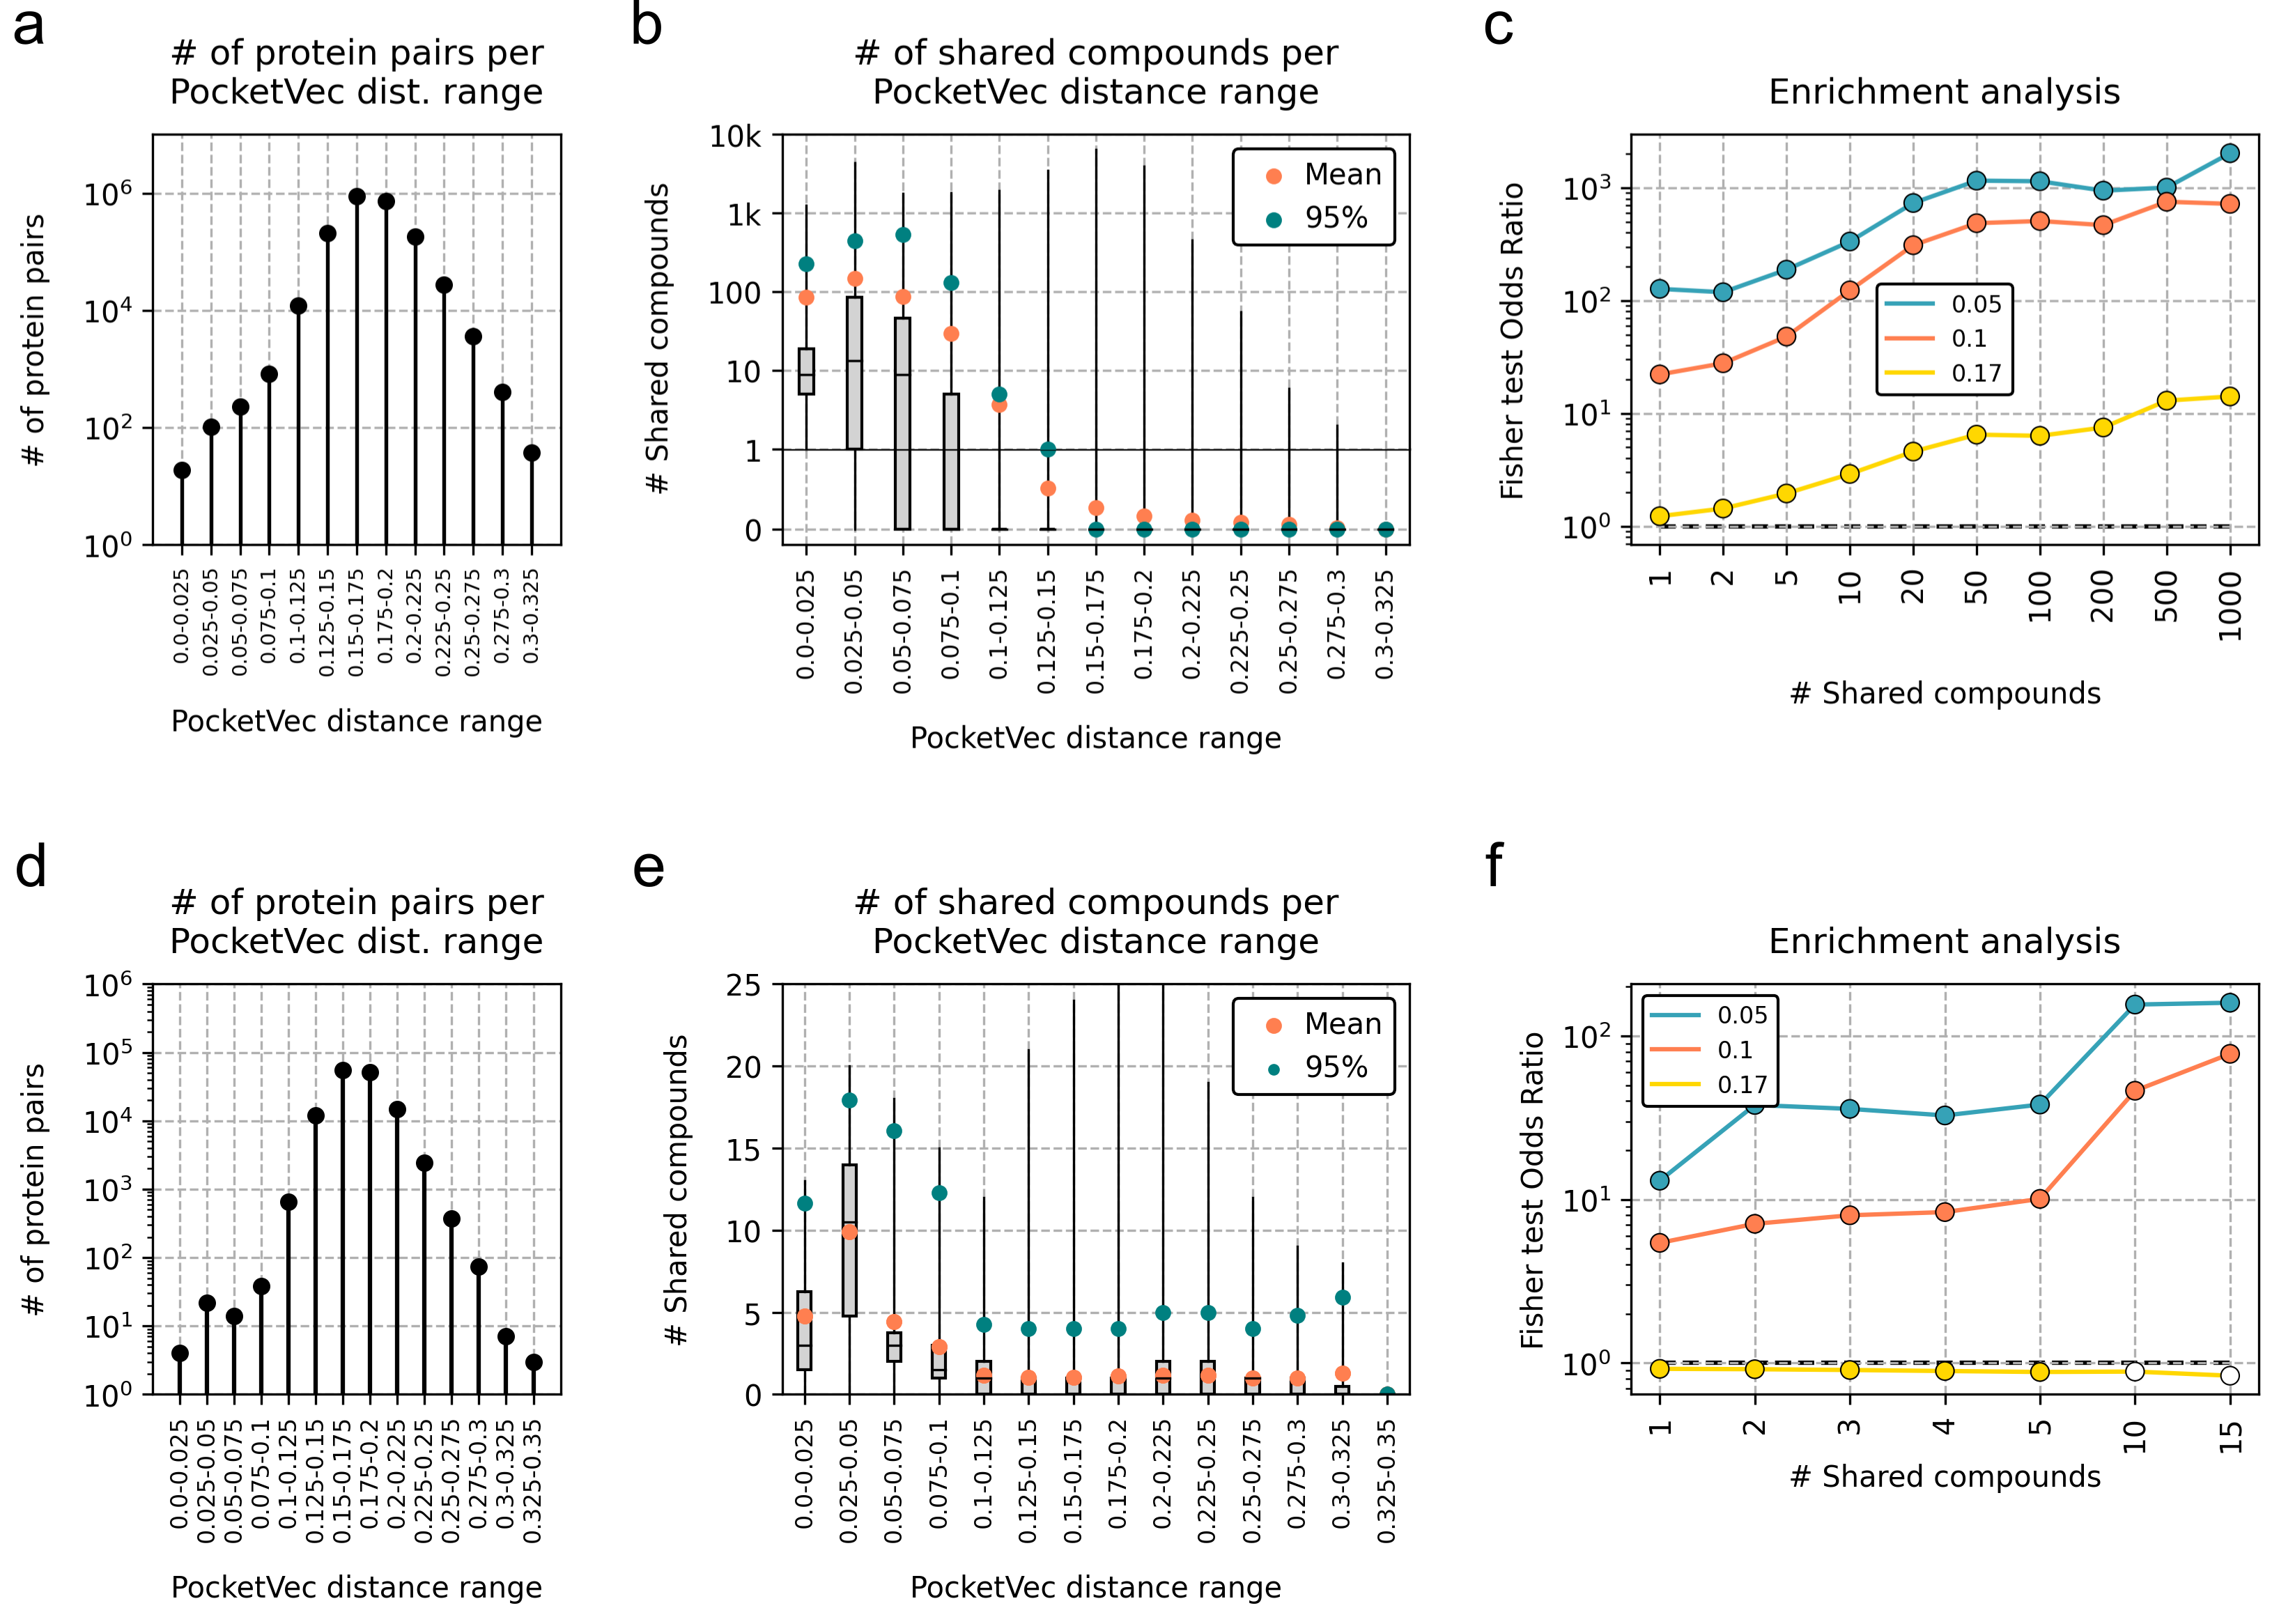
\includegraphics[width=\linewidth]{figures/PocketVec/Main/Fig6.png} 
  \caption{
    \textbf{Relationship between PocketVec similarity and experimentally determined compound-target pairs.}
    All vs All (PDB-LIG, PDB-PD, AF2-LIG and AF2-PD) comparison between PocketVec distance and number of shared compounds among proteins having experimental binding data in ChEMBL and BindingDB (a, b, c) and Offensperger et al.\cite{offensperger_large-scale_2024} (d, e, f).
    \textbf{a, d)} Number of protein pairs (y-axis) at each PocketVec distance range (x-axis).
    \textbf{b, e)} Number of shared compounds for all pairs having a PocketVec distance in the specified distance range. Orange dots indicate the average value while green dots indicate the lower bound for the top 5\% of the pairs. Boxplots indicate median (middle line), 25th, 75th percentile (box), and maximum and minimum values (whiskers). 
    \textbf{c, f)} Evolution of Fisher test Odds Ratio (y-axis) for an increasing number of shared compounds (x-axis) using an increasing value of PocketVec distance cut-off (0.05, 0.10 and 0.17). Colored dots indicate pvalue <0.001, gray dots indicate pvalue <0.05 and white dots indicate pvalue >0.05.
  }
  \rule[0ex]{\textwidth}{0.5pt}
  \vspace{-5mm}
  \label{PocketVec_Fig6}
\end{figure}

%%%%%%%%%%%%%%%%%%%%%%%%%%%%%%%%%%%%%%%%%%%%%%%%%%%%%%%%%%%%%%%%
%%% Identifying kinases with similar inhibition profiles through PocketVec descriptors
%%%%%%%%%%%%%%%%%%%%%%%%%%%%%%%%%%%%%%%%%%%%%%%%%%%%%%%%%%%%%%%%

\phantomsection
\subsubsection{Identifying kinases with similar inhibition profiles through PocketVec descriptors}
\label{PocketVec_ResultsAndDiscussion_Identifying_Kinases}

Protein kinases have long been a cornerstone of drug discovery efforts primarily due to their role as oncogenic targets\cite{attwood_trends_2021}. Since the breakthrough FDA-approval of imatinib in 2001, dozens of small molecules (72 as of November 2022\cite{roskoski_properties_2023}) have been approved as therapeutic kinase inhibitors for clinical use. However, the design of selective inhibitors is a challenging task due to the highly conserved ATP-binding pocket shared among human kinases. Indeed, many kinase inhibitors show high promiscuity (i.e. they bind to many kinases), while others are rather selective\cite{karaman_quantitative_2008, davis_comprehensive_2011}. This same variability is also apparent from the kinase perspective: some bind to many inhibitors while others are extremely selective\cite{hanson_what_2019}. Our characterization of druggable pockets in human proteins showed 1,286 potential binding sites within protein kinase domains. More specifically, we derived PocketVec descriptors for 229, 404, 195 and 458 pockets in the PDB-LIG, PDB-PD, AF2-LIG and AF2-PD sets, respectively. Thus, we set up to explore a potential correlation between the pockets in the different kinases and their experimentally determined small molecule inhibition profiles.

We first collected kinase-inhibitor pairs identified through systematic chemical proteomics approaches by Kuester and collaborators, where they tested interactions between 520 kinases and 243 inhibitors (2017 set)\cite{klaeger_target_2017}, and between 318 kinases and 1,183 inhibitors (2023 set)\cite{reinecke_chemical_2023}. We used a standard activity cutoff of 30nM to define binary kinase-inhibitor matrices, as recommended in Pharos 17 (\href{http://pharos.nih.gov}{http://pharos.nih.gov}). In the 2017 set, we found interactions involving 111 kinases and 94 inhibitors (Fig \ref{PocketVec_Fig7}a), with 43 kinases being inhibited by a single compound, and 18 of them interacting with 5 or more inhibitors (Fig \ref{PocketVec_FigS29}a). In the 2023 set, we identified interactions comprising 73 kinases and 164 inhibitors, where 19 kinases interacted with 1 inhibitor and 27 with 5 or more (Fig \ref{PocketVec_FigS29}b). We then compared kinases on the basis of their binarized inhibition profiles (Jaccard similarity, Fig \ref{PocketVec_Fig7}d, j, upper triangular matrices), and we observed that a relatively small fraction of kinase pairs shared at least 1 inhibitor (12.3\% and 9.7\% for the 2017 and 2023 sets, respectively). We also compared the kinases using PocketVec descriptors (Fig \ref{PocketVec_Fig7}d, j, lower triangular matrices), finding that the fraction of kinase pairs showing similar druggable pockets (i.e. PocketVec distances <0.17) was 40.5\% and 41.4\%, respectively. As expected, these fractions were significantly higher than the figure obtained when comparing random sets of pocket descriptors (\textasciitilde2\%. Fisher’s exact test, OR >30, p-value \textasciitilde0), since all kinases contain at least one similar ATP-binding pocket. Reassuringly, as observed in the general analysis of human druggable pockets (Fig \ref{PocketVec_Fig3}h), we found that the higher the number of common inhibitors between pairs of kinases, the more similar their pockets were according to PocketVec descriptors (Fig \ref{PocketVec_Fig7}b, h). However, even when no shared inhibitor was found for a pair of kinases, as expected, the similarity between their ATP-binding pockets was quite remarkable, suggesting that the PocketVec distance threshold should be lowered to disentangle drug promiscuity.
  

Next, we parsed the general inhibition matrices to derive inhibition profiles for each kinase (i.e. a vector describing whether it does or does not interact with every tested inhibitor), and we assessed the coherence between PocketVec distances and the similarity between experimentally determined inhibition profiles. Indeed, kinase pairs with low PocketVec distances (<0.17) showed a significant enrichment for similar inhibition profiles (Fisher’s exact test, OR = 3.2, p-value <0.0003 in the 2017 set, and OR = 4.1, p-value <0.003 in the 2023 set for a Jaccard similarity >0.5). These enrichments were even more pronounced when we applied more stringent distance thresholds (PocketVec distance <0.10) with OR >118 and OR >125 (p-values <10\textsuperscript{-10}) for the 2017 and 2023 sets, respectively (Fig \ref{PocketVec_Fig7}c, i).

We then compared our results using PocketVec descriptors to more classical structure and sequence similarity analyses (see \hyperref[PocketVec_Methods]{Methods}). As expected, we found that structurally similar proteins (Max. TM-score >0.85) were also moderately enriched in similar inhibition profiles (OR = 2.4, p-value <0.05; OR = 1.7, p-value >0.05), as were kinases sharing >35\% sequence identity (OR = 4.8, p-value <10\textsuperscript{-6}; OR = 5.5, p-value <10\textsuperscript{-4}). Finally, we studied the relationship between structure, sequence, PocketVec and inhibition profile similarity between kinase pairs. Consistently with our global analysis of the human druggable pockets (Fig \ref{PocketVec_Fig5}a), higher structure and sequence similarities consistently led to lower PocketVec distances in both the 2017 (Fig \ref{PocketVec_Fig7}e, f) and the 2023 (Fig \ref{PocketVec_Fig7}k, l) sets.

%%%%%%%%%%%%%%%%
%%% FIGURE 7 %%%
%%%%%%%%%%%%%%%%

% \begin{figurehere}
%   \centering
%   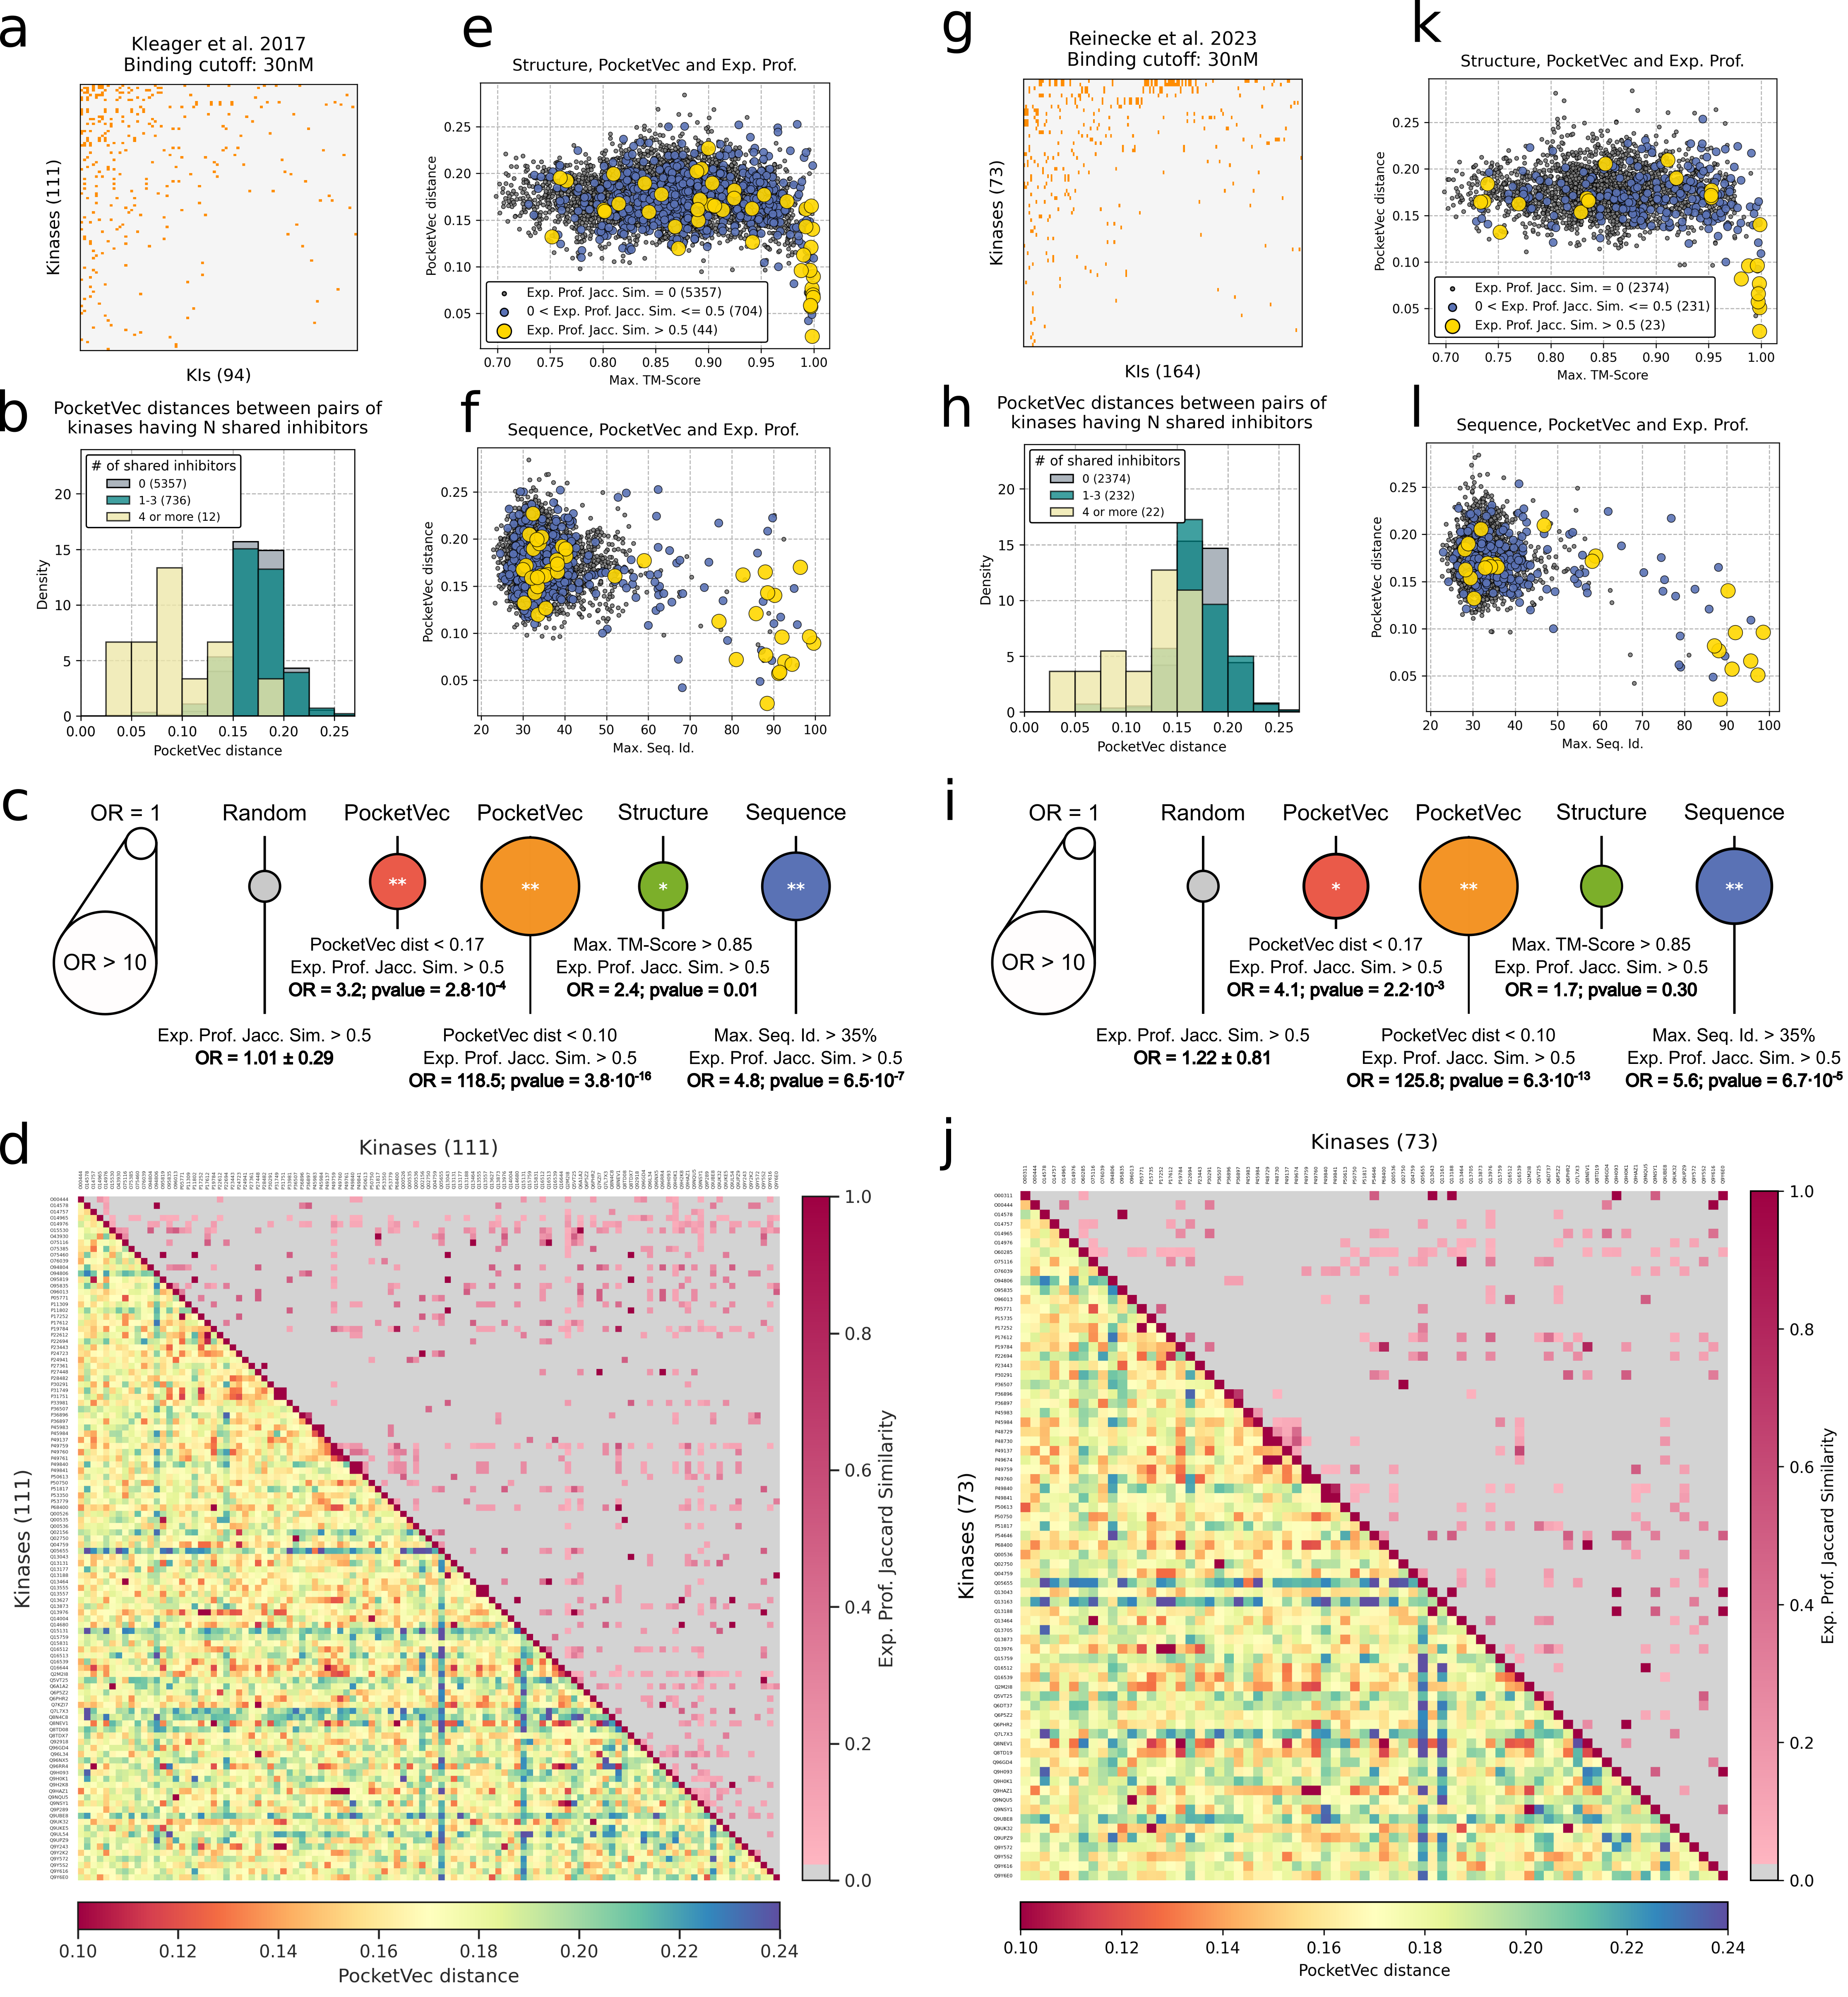
\includegraphics[width=0.8\linewidth]{figures/PocketVec/Main/Fig7.png} 
%   \caption{
%     Correlation between inhibition profiles and PocketVec descriptors. All the analyses have been performed on the data obtained from Kleager et al.\cite{klaeger_target_2017} (right panels) and Reinecke et al.\cite{reinecke_chemical_2023} (left panels).
%     \textbf{a, g)} Inhibition matrix between protein kinases, and small molecule kinase inhibitors binarized at 30 nM. Both kinases and inhibitors are sorted by the number of active inhibition events. Orange dots indicate inhibition and white dots indicate no inhibition.
%     \textbf{b, h)} Distributions of PocketVec distances grouped by the number of shared inhibitors between kinases (0, 1-3 and 4 or more). The number of kinase pairs per number of shared inhibitors is specified in parenthesis.
%     \textbf{c, i)} Enrichments (Fisher’s exact test) in similar inhibition profiles (Jaccard Similarity >0.5) for those kinase pairs being similar in terms of PocketVec distance (red: <0.17, orange: <0.10), structural similarity (TM-score >0.85) and sequence identity (>35\%). For comparison, the results obtained with randomly selected kinase pairs (gray) are also included. Circle areas are proportional to the corresponding ORs and p-values are specified in the center with the following format: * p-value < 0.05, ** p-value < 0.001.
%     \textbf{d, j)} Pairwise kinase comparisons. Rows and columns correspond to alphabetically sorted kinases (by Uniprot ID). Upper triangular matrices: kinases are compared on the basis of their experimentally determined inhibition profiles. Each square represents the Jaccard similarity between the inhibition profiles of two targets: the higher the Jaccard similarity, the more similar the corresponding inhibition profiles. Lower triangular matrices: kinases are compared on the basis of their PocketVec descriptors (employing the minimum distance among all PocketVec descriptors in the Protein Kinase Domains). The color of each square indicates the minimum PocketVec distance between two targets: the lower the PocketVec distance (red), the more similar the kinases are at pocket level according to our descriptors.
%     \textbf{e, k)} Relationship between structural similarity (x-axis, Max. TM-score) and PocketVec distances (y-axis) between pairs of protein kinases. Each point represents a kinase pair and is colored and sized in terms of the similarity between experimentally determined inhibition profiles.
%     \textbf{f, l)} Relationship between sequence similarity (x-axis, Max. Seq. Id.) and PocketVec distances (y-axis) between pairs of protein kinases. Each point represents a kinase pair and is colored and sized in terms of the similarity between experimentally determined inhibition profiles.
%     \label{PocketVec_Fig7}
%   }
% \end{figurehere}

\begin{Figure_modified}
 \begin{center}
  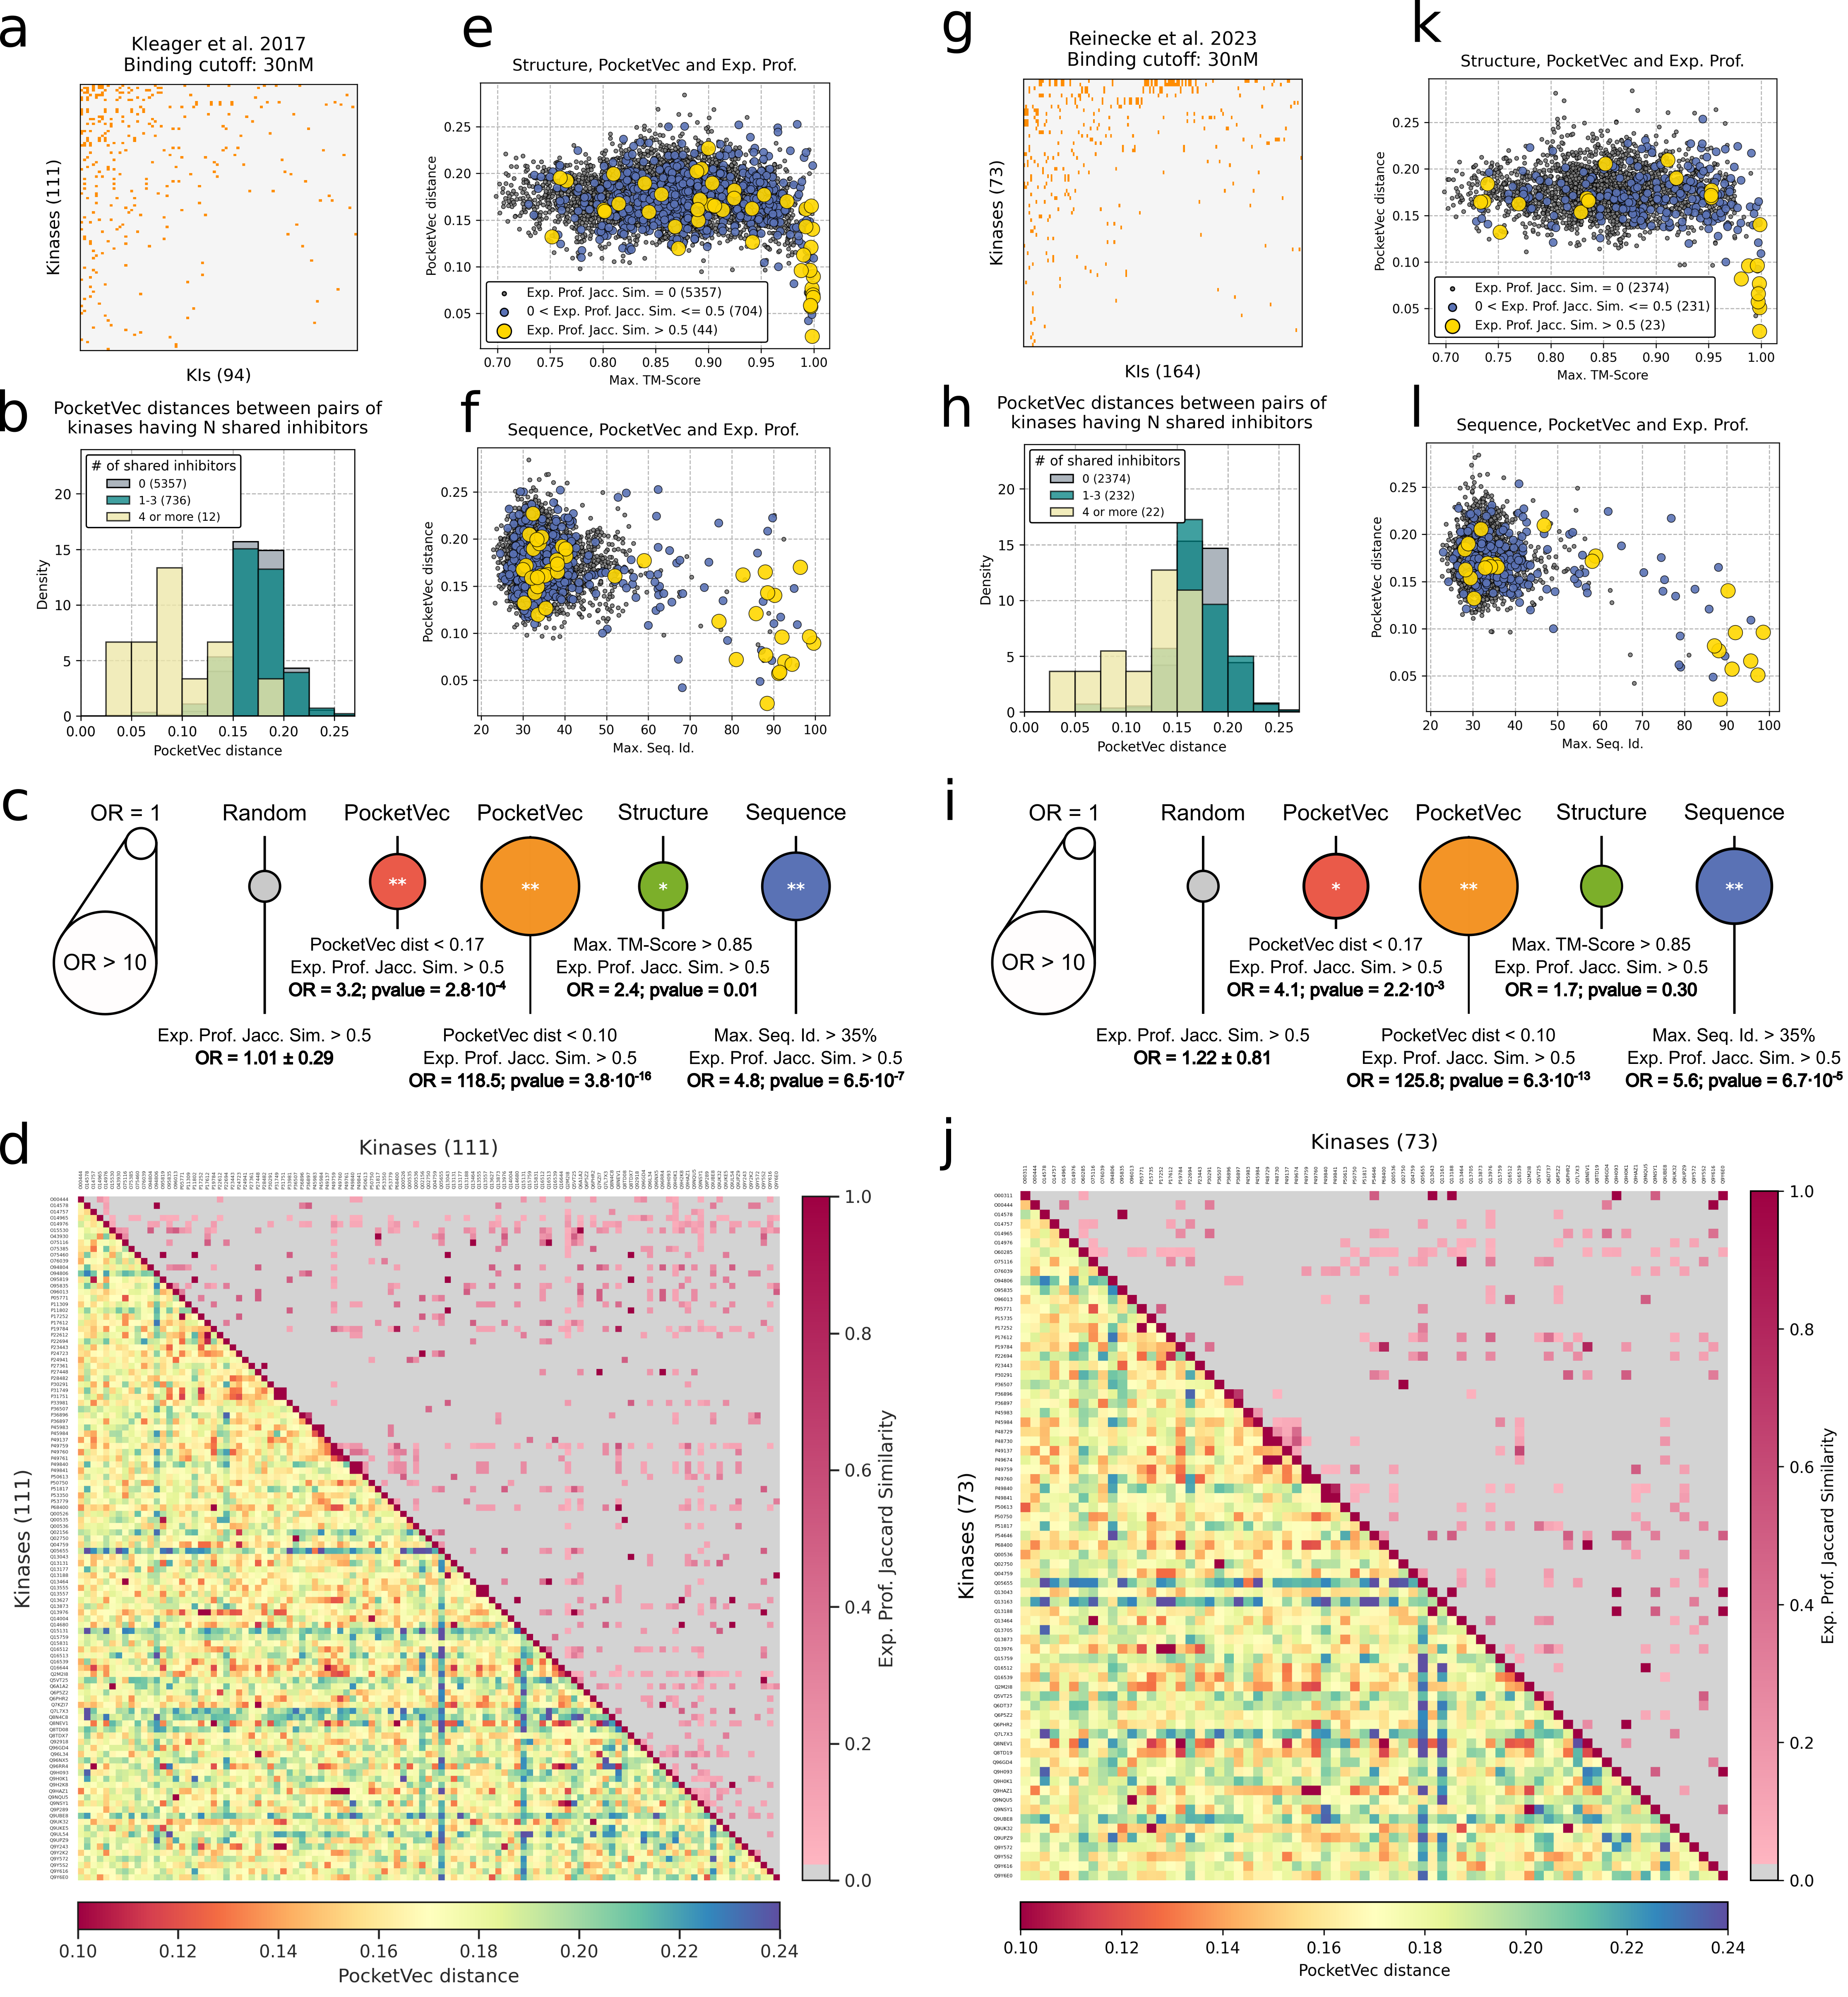
\includegraphics[width=1\textwidth]{figures/PocketVec/Main/Fig7.png}
  \caption{\textbf{Correlation between inhibition profiles and PocketVec descriptors.} All the analyses have been performed on the data obtained from Kleager et al.\cite{klaeger_target_2017} (right panels) and Reinecke et al.\cite{reinecke_chemical_2023} (left panels).
    \textbf{a, g)} Inhibition matrix between protein kinases, and small molecule kinase inhibitors binarized at 30 nM. Both kinases and inhibitors are sorted by the number of active inhibition events. Orange dots indicate inhibition and white dots indicate no inhibition.
    \textbf{b, h)} Distributions of PocketVec distances grouped by the number of shared inhibitors between kinases (0, 1-3 and 4 or more). The number of kinase pairs per number of shared inhibitors is specified in parenthesis.
    \textbf{c, i)} Enrichments (Fisher’s exact test) in similar inhibition profiles (Jaccard Similarity >0.5) for those kinase pairs being similar in terms of PocketVec distance (red: <0.17, orange: <0.10), structural similarity (TM-score >0.85) and sequence identity (>35\%). For comparison, the results obtained with randomly selected kinase pairs (gray) are also included. Circle areas are proportional to the corresponding ORs and p-values are specified in the center with the following format: * p-value < 0.05, ** p-value < 0.001.
    \textbf{d, j)} Pairwise kinase comparisons. Rows and columns correspond to alphabetically sorted kinases (by Uniprot ID). Upper triangular matrices: kinases are compared on the basis of their experimentally determined inhibition profiles. Each square represents the Jaccard similarity between the inhibition profiles of two targets: the higher the Jaccard similarity, the more similar the corresponding inhibition profiles. Lower triangular matrices: kinases are compared on the basis of their PocketVec descriptors (employing the minimum distance among all PocketVec descriptors in the Protein Kinase Domains). The color of each square indicates the minimum PocketVec distance between two targets: the lower the PocketVec distance (red), the more similar the kinases are at pocket level according to our descriptors.
    \textbf{e, k)} Relationship between structural similarity (x-axis, Max. TM-score) and PocketVec distances (y-axis) between pairs of protein kinases. Each point represents a kinase pair and is colored and sized in terms of the similarity between experimentally determined inhibition profiles.
    \textbf{f, l)} Relationship between sequence similarity (x-axis, Max. Seq. Id.) and PocketVec distances (y-axis) between pairs of protein kinases. Each point represents a kinase pair and is colored and sized in terms of the similarity between experimentally determined inhibition profiles.
 }
  \vspace{-5mm}
  \rule[0ex]{\textwidth}{0.5pt}
  \vspace{-9mm}
 \label{PocketVec_Fig7}
 \end{center}
\end{Figure_modified}

Despite the coherence of the results of the three metrics, interestingly, we found 9 kinase pairs (4 in the 2017 and 5 in the 2023 sets) with clear inhibition profile similarities that only PocketVec descriptors could pick. On the other hand, our analyses also revealed 8 cases (5 in the 2017 and 3 in the 2023 sets) where PocketVec descriptors fell short to detect similarities that could be recovered by sequence or structure comparisons alone. Overall, these results emphasize the coherence and complementarity between strategies, highlighting the potential of PocketVec descriptors to identify otherwise unattainable similarities in experimental inhibition profiles among protein kinases. 
\subsection{Code and data availability}
\label{PocketVec_Code}

All the code necessary to generate PocketVec descriptors for any pocket of interest is available in our GitLab (\href{https://gitlabsbnb.irbbarcelona.org/acomajuncosa/pocketvec}{https://gitlabsbnb.irbbarcelona.org/acomajuncosa/pocketvec}), together with installation instructions and guidelines for running the code. On average, the generation of a PocketVec descriptor for a protein pocket takes 1h on an Intel Xeon Gold 6138 CPU.

In addition, in the same repository under the results directory, we also provide all the pre-computed descriptors and the comparisons with sequence and structure similarity measurements, as described in the text.



\subsection{Concluding remarks}

We have presented PocketVec, a novel approach to generate vector-like protein pocket descriptors based on inverse docking and the chemogenomics principle that similar pockets bind similar ligands. A thorough assessment of its performance ranks it among the best available methodologies to characterize and compare protein druggable pockets, while overcoming some important limitations. We have also systematically searched for druggable pockets in the folded human proteome, using experimentally determined protein structures and AF2 models, identifying over 32,000 binding sites in more than 20,000 protein domains. We then derived PocketVec descriptors for each small molecule binding site and took advantage of their vector-like format to run an all-against-all pocket similarity search, exploring over 1.2 billion pairwise comparisons. Besides, we provide pre-computed descriptors for every identified human pocket together with the annotated Python code to generate new descriptors for any pocket of interest. We found that PocketVec descriptors are complementary to other, more classical, search strategies, enabling the identification of pocket similarities not revealed by structure- or sequence-based comparisons. As illustrative examples of applicability, we unveiled a clear relationship between pocket similarities, as defined by low PocketVec distances, and the probability of those pockets to bind the same compounds, as experimentally detected. Moreover, a systematic comparison of druggable pockets in protein kinases showed that kinase pairs with similar PocketVec descriptors also exhibited similar experimentally determined inhibition profiles. 

There have been recent attempts to identify druggable pockets at the proteome level\cite{wang_cavityspace_2022, konc_probis-fold_2022, sim_hproteome-bsite_2022, tsuchiya_possum_2023}. However, the novelty of our ligand-centric methodological approach, the accuracy of our descriptors and the systematic and exhaustive identification and characterization of binding pockets enabled the analyses of the effects of protein structural variation on pocket definition and small molecule binding at an unprecedented scale. Besides, the comprehensive list of human-derived pocket descriptors will become a valuable resource for the bio and cheminformatics communities.

This first generation of descriptors has been primarily designed for global analyses, such as the comprehensive characterization of all human druggable pockets. Indeed, our analyses have revealed dense clusters of similar pockets in distinct proteins for which no inhibitor has yet been co-crystalized, opening the door to strategies to prioritize the development of chemical probes to cover the druggable space\cite{carter_target_2019}. Moreover, our initial descriptors can be easily adapted to cater to specific tasks (i.e. exploring substrate specificity in a given protein family) by refining the selection of predefined lead-like molecules used or fine-tuning the similarity cutoff, thereby enhancing their performance. Of special interest are the anticipation of undesired off-targets as well as the guidance of rational polypharmacology, where single univalent molecules could be designed to target two proteins simultaneously, provided that their druggable pockets are similar enough\cite{duran-frigola_detecting_2017}. However, the main impact is likely to come from proteochemometric approaches, where a combination of ligand and target descriptors are used to train machine learning models\cite{fernandez-torras_connecting_2022}. It has been shown that structure-based descriptors of the targets are often superior to distinguish drug selectivity, although the sequence-based ones are usually used when key protein structural details are lacking\cite{bongers_proteochemometrics_2019}. The generation of accurate descriptors derived for not yet described pockets in AF2 protein models overpasses this limitation, and opens up many possibilities. We envisage a scenario where small molecule and pocket descriptors combined are used to train AI-based generative models (e.g. to design new chemical entities that bind each protein druggable cavity\cite{jin_hierarchical_2020, blaschke_reinvent_2020}). Indeed, the estimated space of 10\textsuperscript{33} synthetically accessible drug-like molecules is mostly unexplored and represents a reservoir of potentially bioactive compounds\cite{polishchuk_estimation_2013}. Deep learning strategies have successfully designed new antibiotic scaffolds\cite{wong_discovery_2024} and placed 15 AI-designed drugs in clinical trials, including first-in-class molecules against several targets\cite{jayatunga_ai_2022}. Overall, accurate descriptors of druggable pockets might serve as a cornerstone for the development of generative AI approaches in drug discovery, offering unprecedented opportunities to expedite the design of a chemical toolbox to probe biology and, ultimately, to new therapeutics.
\subsection{Methods}
\label{PocketVec_Methods}

\phantomsection
\subsubsection{Selection of compound sets}

Fragments: we downloaded the Glide\cite{friesner_glide_2004, halgren_glide_2004} diverse fragment dataset from the Schrodinger website (\href{https://www.schrodinger.com}{https://www.schrodinger.com}) in November 2020. This collection of compounds is composed of 667 molecules having molecular weights in the 50-200 g·mol\textsuperscript{-1} range (Fig \ref{PocketVec_FigS2}).

Lead-like molecules (LLM): we retrieved a set of 650k lead-like molecules from MOE v2019.01 (Chemical Computing Group, Montreal, Canada). We then performed a k-means clustering using TAT fingerprints, setting the number of clusters to 1,000, and selected the corresponding 1,000 molecules closest to each cluster centroid to build the library. These compounds exhibit molecular weights in the 200-450 g·mol\textsuperscript{-1} range (Fig \ref{PocketVec_FigS2}). 

\phantomsection
\subsubsection{Small molecule docking strategies}

Rigid docking: we performed rigid docking calculations using rDock\cite{ruiz-carmona_rdock_2014} (downloaded on July 2021 from \href{https://github.com/CBDD/rDock}{https://github.com/CBDD/rDock}). We prepared the protein structures using MOE v2019.01 (Chemical Computing Group, Montreal, Canada), Biopython\cite{cock_biopython_2009} and the structure checking utility from BioExcel Building Blocks\cite{andrio_bioexcel_2019}. We ran all docking calculations using standard parameters and scoring functions. The binding site box was built around the pocket centroid (ligand centroid or detected pocket centroid) with a radius of 12 Å (RbtLigandSiteMapper option) and the number of runs was set to 25. Finally, we set the DIHEDRAL\_MODE to FIXED (rigid docking). The considered score for each molecule was the minimum value of SCORE.INTER.

Flexible docking: we used SMINA\cite{koes_lessons_2013} (downloaded on November 2020 from \href{https://sourceforge.net/projects/smina}{https://sourceforge.net/projects/smina}) for the flexible docking calculations. We prepared the protein structures using Reduce\cite{word_asparagine_1999}, OpenBabel\cite{oboyle_open_2011}, Biopython\cite{cock_biopython_2009} and the structure checking utility from BioExcel Building Blocks\cite{andrio_bioexcel_2019}. We ran all the calculations using standard parameters and scoring functions for flexible docking. The binding site box was automatically derived from the position of the bound ligand (autobox\_ligand parameter). The considered score for each molecule was the minimum value of \textit{minimized\_affinity}. 


\phantomsection
\subsubsection{Post-docking analysis}

For each pocket under evaluation, docking scores were stored in a one-dimensional NumPy array\cite{harris_array_2020} and then translated into rankings using SciPy\cite{virtanen_scipy_2020} (\textit{rankdata} function, method \textit{max}). In this way, the molecule with the lowest docking score was assigned the top ranking (1\textsuperscript{st}), while the one with the highest docking score was ranked as the N\textsuperscript{th} (being N the total number of tested molecules; N=128 in the standard PocketVec pipeline). It is important to note that molecules yielding positive docking scores (e.g. due to structural clashes with the protein) were not explicitly considered and their corresponding rankings were set to an outlier value (e.g. 129). The rationale behind this procedure was that such outlier molecules were indeed informative (i.e. the pocket was too small to fit them) but needed to be distinguished from binders having poor (but negative) docking scores (i.e. weak binders). Specifically, docking scores in the range 0-50, 50-100 and >100 were translated into N+1, N+2 and N+3 rankings, respectively (129, 130, 131 in the standard PocketVec pipeline).

\phantomsection
\subsubsection{Benchmark set}

A good strategy to identify the best combination of small molecules and docking methods to develop pocket descriptors, and to assess their validity, is to see if they can faithfully capture reported similarities between small molecule binding pockets. To this end, we used ProSPECCTs\cite{ehrt_benchmark_2018}, a collection of 10 datasets composed of protein-ligand binding site pairs classified as similar or dissimilar according to specific criteria (downloaded in July 2021 from \href{http://www.ewit.ccb.tu-dortmund.de/ag-koch/prospeccts/}{http://www.ewit.ccb.tu-dortmund.de/ag-koch/prospeccts/}). P1 (P1.2) includes 326 (45) protein-ligand complexes involving 12 (12) different proteins, and it is meant to study the sensitivity of pocket comparison tools to the binding site definition by comparing proteins having identical sequences with chemically distinct (similar) ligands located at the same site. P2 comprises 17 PDB files resolved by NMRs, containing a total of 329 different models, and was designed to assess the impact of protein flexibility in pocket comparisons. P3 and P4 include a variable number (1 to 5) of randomly added artificial mutations in the P1 proteins leading to changes in the physicochemical (P3) and physicochemical and shape (P4) properties of the protein binding site. For the sake of simplicity and coherence with reported performances, we have only considered structures with 5 mutations (representing 326 out of 1630 mutated structures). P5 (P5.2) was designed to detect pairs of unrelated proteins binding to identical or similar ligands, and consists of 80 (100, including phosphate binding sites) protein-ligand complexes\cite{kahraman_shape_2007}. P6 (P6.2) is intended to evaluate the identification of distant relationships between pockets binding to identical ligands but having variable pocket environments\cite{barelier_recognition_2015}, and it includes 115 protein structures excluding (including) cofactors. We did not use P6 or P6.2 to benchmark our methodology since all pocket pairs are bound to identical or highly similar ligands, and the similar/dissimilar classification is done considering fine details of protein-ligand binding, such as the involved ligand functional groups. Thus, this set is not appropriate to guide and assess the developments of our pocket descriptors. Finally, P7 was retrieved from published successful applications of pocket similarity studies in a diverse set of proteins, and it contains 1,151 protein structures. A detailed overview of all ProSPECCTs datasets is presented in Fig \ref{PocketVec_FigS3}.

\phantomsection
\subsubsection{Entropy measurements}

For each molecule within each ProSPECCTs dataset, rankings were first binned into 100 different groups (bins) in order to discretize a variable (rankings) that, in practical terms, was continuous (since ranking range was usually higher than the number of considered structures). Shannon's Entropy was then calculated using such binned data (SciPy\cite{virtanen_scipy_2020}, entropy function, base 2).

\phantomsection
\subsubsection{Domain-based characterization of the human druggable pockets}

We searched all human protein identifiers from UniProt (July 2022, \textit{organism\_id 9606} and \textit{reviewed} set to \textit{true}), retrieving a total of 20,386 unique human proteins\cite{the_uniprot_consortium_uniprot_2023}. Then, for each human protein, we retrieved all Pfam domains\cite{mistry_pfam_2021}, considering only those entities labeled as ‘domain’ (e.g. we did not include ‘repeats’). Overall, we found 28,044 domains (2,704 unique Pfam domains) in 11,242 human proteins (Fig \ref{PocketVec_Fig2}a and Fig \ref{PocketVec_FigS15}).

To structurally annotate these domains, we used two different strategies. On the one hand, we looked for experimentally determined structures searching the PDB\cite{goodsell_rcsb_2020}. For each human domain, we gathered all PDB chains showing a structural coverage of the domain ≥80\% using the localpdb package\cite{ludwiczak_localpdb_2022} (PDB version 2022.02.25). We identified at least one PDB structure for 7,774 domains (1,839 unique Pfam domains in 4,726 proteins), processing all PDB files and removing those regions outside the domains under study. Additionally, we downloaded all predicted structures for Homo Sapiens from AlphaFold DB (\href{https://alphafold.ebi.ac.uk/download\#proteomes-section}{https://alphafold.ebi.ac.uk/download\#proteomes-section}, proteins having <2,700 amino acids, August 2022), processed all files and removed those regions that did not match the domains under study, leaving predicted structures for 25,589 domains (2,671 unique Pfam domains in 11,022 proteins).

To identify druggable pockets, we also followed two complementary strategies.

a) Ligand--based. In the ligand-based pocket definition, we identified all the PDB structures (chains) corresponding to human protein domains that contained small molecules (HET PDB codes) co-crystallized with the domains of interest that fulfilled the following criteria: i) being annotated as ligands in PDBSUM\cite{laskowski_pdbsum_2018} data, ii) not being one of the 20 naturally occurring amino acids, iii) having a number of carbon atoms >6, to filter out solvent molecules and crystallography-related species and vi) having solvent accessibility ≤0.4 or buriedness ≥15. We defined solvent accessibility as the ratio between the ligand solvent-accessible surface area (SASA) in the bound state and the ligand SASA in the free state. SASA values were calculated with RDKit (\href{https://www.rdkit.org}{https://www.rdkit.org}). Additionally, we defined buriedness as the number of protein residues having a distance below 8Å to the ligand centroid, and we calculated these values using Biopython\cite{cock_biopython_2009}. The cut-off values for accessibility (0.4) and buriedness (15) were set upon visual inspection of many bound ligands. We considered both parameters in order to recover as many interesting cases as possible: accessibility values usually underestimated pockets defined by small ligands while buriedness values often underrated large pockets. By applying all these conditions, we made sure to consider only pharmacologically relevant small molecules while filtering out inorganic chemicals, short peptides and crystallization additives such as ethylene glycol (EDO), glycerol (GOL), polyethylene glycol (PEG) and DMSO (DMS), among many others. In total, we found at least one PDB structure containing a ligand fulfilling all conditions for 1,279 domains (363 unique Pfam domains in 1,205 proteins). For 503 of these, we only found a single ligand, whereas for 254 of them we could find 10 or more ligands (Fig \ref{PocketVec_FigS16}), including a variety of metabolic nucleotides such as ADP (found in 114 domains, Fig \ref{PocketVec_FigS30}) or GDP (found in 102 domains, Fig \ref{PocketVec_FigS30}).

To compile the list of unique ligand-defined pockets we followed the procedure shown in Fig \ref{PocketVec_Fig2}a. First, we chose a reference PDB structure for each protein domain where we considered the structural coverage of the domain and the resolution of the crystal structure. We then superimposed all domain structures with the corresponding bound ligands onto their reference structure using TM-align\cite{zhang_tm-align_2005}. 

To define a final set of ligand-based druggable pockets per domain, we used a single-linkage clustering technique, merging into a single pocket all those ligands whose centroids were at a distance ≤5Å while maintaining the maximum distance between the global centroid of the cluster and the centroids of the individual compounds ≤18Å. We considered the final global cluster centroids as the pocket centroids. Overall, we found 1,604 ligand-defined pockets in 1,279 protein domains (363 unique Pfam domains in 1,205 proteins). We named this set of pockets \textbf{PDB-LIG}.

We then superimposed the reference PDB structure of the previous domains to their AF2 predicted counterparts by means of TM-align\cite{zhang_tm-align_2005}, and transferred the location of the identified PDB-LIG pockets. We only considered those pockets having a pLDDT value >70 for all the residues at a distance ≤8Å from the pocket centroid. Overall, we identified 1,405 pockets in 1,131 domains (339 unique Pfam domains in 1,074 proteins), and named this set of pockets \textbf{AF2-LIG}.

b) Pocket--detection. As a complementary strategy, and to increase the overall coverage of human druggable pockets, we attempted a \textit{de novo} identification of pockets. To establish a standardized protocol to predict them, we assessed the accuracy of different methods when identifying the PDB-LIG pockets defined above. In brief, we first removed bound ligands from reference \textit{holo} structures (1,279 PDB structures, one per domain) and used Fpocket\cite{le_guilloux_fpocket_2009} and P2rank\cite{krivak_p2rank_2018}, two state-of-the-art methods, to detect pockets in ligand-free domain structures. Additionally, we also used Prank\cite{krivak_improving_2015}, a functionality of P2rank aimed at rescoring the pockets predicted by Fpocket. In this way, we benchmarked three different strategies to detect and score domain binding sites. We considered that a predicted pocket and a ligand-defined pocket matched if the distance between their centroids was ≤6.14Å, which corresponded to the 95\textsuperscript{th} percentile of the distribution of all pairwise distances between ligand centroids within each cluster in the PDB-LIG set (Fig \ref{PocketVec_FigS31}). We found that only 0.18\% and 0.56\% of Fpocket and P2rank predicted pocket pairs, respectively, had a distance between their centroids below that value. Given the apparent over-prediction of pockets of the two methods, we explored the precision/recall balance when keeping only the top scoring predicted pockets. Overall, we found that the best strategy to detect real binding sites in ligand-free structures was the combination of Fpocket detection and Prank scoring. Using the mentioned distance cut-off (6.14Å) and considering the top-2 best scored pockets for each domain, we were able to detect 72\% of the real pockets while 47\% of detected pockets were indeed real (Fig \ref{PocketVec_Fig2}b).

Thus, we first ran Fpocket on the \textit{apo} PDB reference structure for each domain to identify potential druggable pockets, we then ranked them by means of Prank, and we finally kept the top-2 ranked pockets per domain. Overall, this accounted for a total of 14,413 predicted pockets in 7,403 domains (1,806 unique Pfam domains in 4,643 proteins). We named this set of pockets \textbf{PDB-PD}.

We then used the same strategy and criteria as before to detect pockets onto the predicted AF2 domain structures (Fpocket and Prank combination filtering out those pockets having residues with pLDDT values <70), annotating a total of 32,202 pockets in 19,211 domains (2,409 unique Pfam domains in 10,314 proteins). We named this set of pockets \textbf{AF2-PD}.

For each pocket and structure, we calculated pocket volume and buriedness using the rDock CAVITY functionality\cite{ruiz-carmona_rdock_2014} and BioPython\cite{cock_biopython_2009}, respectively.

\phantomsection
\subsubsection{Assessment of the effect of protein flexibility}

To exhaustively assess the behavior of PocketVec descriptors upon protein flexibility and conformational changes, from the PDB-LIG set, we selected those pockets for which we had i) ≥10 experimental structures with a co-crystallized ligand (i.e. \textit{holo}), ii) ≥10 experimental structures without a ligand (i.e. \textit{apo}) and iii) and AF2 structure with pLDDT <70 for all residues at a distance <8Å from the pocket centroid. To avoid biasing the results towards overrepresented pockets, we capped the number of selected PDB structures to 10 in both cases (\textit{holo} and \textit{apo}). Overall, we kept 43 pockets and generated PocketVec descriptors for 10 of their \textit{holo} structures, 10 of their \textit{apo} structures and the corresponding AF2 model, resulting in a total number of 903 PocketVec descriptors (43 pockets x 21 descriptors).

Additionally, we gathered MD data from ATLAS\cite{vandermeersche_atlas_2024}, a repository of standardized MD simulations for 1,390 PDB chains including their calculated trajectories as well as several quantitative analyses. In PDB-LIG (PDB-PD), we found available MD trajectories for 7 (96) of their 1,279 (7,403) domains, encompassing 8 (184) pockets. For each domain (103) we randomly sampled 9 MD frames from ATLAS trajectories (3 random frames per replica, x3 replicas), using the corresponding TPR and XTC GROMACS files. Thus, for each pocket (192), we considered 10 individual structures: the original one from the PDB-LIG/PDB-PD set and 9 frames from the MD simulations. Then, for each pocket, we calculated all pairwise distances (45) among their PocketVec descriptors (10) and compared them with background distances against each of the 4 sets of PocketVec descriptors we already precompiled (i.e. PDB-LIG, PDB-PD, AF2-LIG, AF2-PD).

\phantomsection
\subsubsection{Assessment of the effect of metals binding proteins}

To assess the ability of our precomputed PocketVec descriptors to identify pocket similarities among metal-binding proteins, such as histone deacetylases (HDACs) or matrix metalloproteinases (MMPs), we first collected all domains within the PDB-LIG and PDB-PD sets (7,399) and kept only those having a metal atom (AU, MN, NA, CU, AG, CO, PB, RB, K, SR, FE, MG, CD, NI, HG, CA, PT, TI, ZN or CS) in at least 1 associated PDB chain (3,568). For further analysis, we only considered those PDB-LIG and PDB-PD pockets that were included within one of these domains (1,052 out of 1,594 and 6,882 out of 14,368, respectively). After that and, for each pocket within each set, we individually considered whether any of the associated PDB chains had a metal atom at a distance <6.14Å from the pocket centroid. For those that indeed had at least 1 metal atom (244 and 785 pockets for the PDB-LIG and PDB-PD sets, respectively) we kept it (if it was on the domain reference structure) or superimposed it (randomly selected from associated PDB chains) against the domain reference structure, and generated PocketVec descriptors for them with the explicit presence of the metal atom. 


\phantomsection
\subsubsection{Systematic comparison of druggable pockets within domain families}

First, for each pair of pockets within the AF2-PD and AF2-LIG sets that were located at the same Pfam domains, we computed the correlation between PocketVec similarity (defined as 1-PocketVec distance), sequence identity and Cα RMSD among pockets. We selected a maximum of 10 protein domains per Pfam domain to avoid biasing the results towards the most frequently occurring ones. We then removed those domain pairs having a global TM-score <0.5 and we performed all pairwise residue mappings using the corresponding Pfam multiple sequence alignments (MSA). After that, pockets (residues <8Å to the pocket centroid) were compared on the basis of their sequences and structures (sequence identity and RMSD Cα, respectively). In fact, we only considered those pocket pairs having a sequence alignment coverage ≥80\% and a centroid distance <6.14Å after domain structural alignment, to account for structural variability (see \textit{Pocket detection} in the previous section).

Additionally, we also ran an all-against-all comparison of pockets in the human pocketome (e.g. PDB-LIG, PDB-PD, AF2-LIG and AF2-PD). Global domain structures were compared using TM-align\cite{zhang_tm-align_2005} (Cα RMSD, TM-score), while domain sequence identities were calculated using global pairwise alignments in BioPython\cite{cock_biopython_2009} (Needleman-Wunsch algorithm, BLOSUM62, gap opening = −10, gap extension = −0.5). 

\phantomsection
\subsubsection{Relationship between PocketVec similarity and experimentally determined compound-target pairs}

We obtained raw binding data from the Chemical Checker (v.2024) compound-target space\cite{duran-frigola_extending_2020}, which contains experimental data on 836,654 compounds bound to 6,933 protein targets, as collected from ChEMBL v.33\cite{zdrazil_chembl_2024} and BindingDB v.2024\cite{gilson_bindingdb_2016}. We also collected all PocketVec descriptors from our study (i.e. PDB-LIG, PDB-PD; AF2-LIG and AF2-PD), encompassing a total number of 10,539 proteins. Of these, we had binding data for 2,028 proteins. We then evaluated the corresponding 2,055,378 protein pairs on the bases of the number of shared compounds (in ChEMBL and BindingDB) and the cosine distances between their PocketVec descriptors.

We then calculated the number of protein pairs within each range of PocketVec distances in an all-vs-all comparison of PocketVec descriptors where, for each protein pair, we kept the minimal distance between PocketVec descriptors, regardless of their set of origin (e.g. PDB-LIG, AF2-PD, etc). Additionally, we depicted the number of shared compounds between each protein pair plotted against the minimal PocketVec distance between each pair and, finally, we calculated the Fisher test odds ratio considering a varying number of shared compounds for a PocketVec distance ≤0.17, ≤0.10 and ≤0.05.

We also performed a similar analysis on the fragment-protein binding pairs recently presented\cite{offensperger_large-scale_2024}, where Winter and co-workers comprehensively tested the potential binding of 407 fragment compounds on 5,951 proteins. We applied the filtering criteria defined by the authors in the original manuscript (i.e. log2 fold change >2.3, median normalized log2 fold change >1, p value <0.05 and adjusted p value <0.25) and we ended up with a binary interaction matrix comprising 332 fragment compounds and 2,744 proteins. As also indicated by the authors, we further removed proteins that were frequent hitters (>40 active fragments) as well as those that were rarely hit (<4 active fragments), restricting our analyses to 301 fragment compounds and 525 proteins for which we had PocketVec descriptors. 


\phantomsection
\subsubsection{Comparison of kinase inhibition profiles with PocketVec descriptors, sequence and structure similarity measurements}

We collected experimentally determined binding affinities from Klaeger et al.\cite{klaeger_target_2017} and Reinecke et al.\cite{reinecke_chemical_2023} (Table \ref{PocketVec_TableS2}). We considered undefined measures as inactive, and low-confidence and high-confidence measures were binarized at 30 nM (as recommended in Pharos\cite{nguyen_pharos_2017}). We then removed all compounds that did not inhibit any kinase and all protein kinases that did not have any inhibitor or any PocketVec descriptor in the Protein Kinase Domain (Pfam PF00069). In this way, we eventually defined a binary inhibition matrix between 111 protein kinases and 94 small molecule kinase inhibitors for Klaeger et al. (Fig \ref{PocketVec_Fig7}a and Table \ref{PocketVec_TableS2}a) and between 73 kinases and 164 inhibitors for Reinecke et al. (Fig \ref{PocketVec_Fig7}b and Table \ref{PocketVec_TableS2}b).

We pairwise compared protein kinases on the basis of their binarized inhibition profiles (Jaccard similarity) and their PocketVec descriptors (employing the minimum distance among all PocketVec descriptors within their Protein Kinase Domains PF00069). Additionally, we also performed sequential and structural comparisons between kinases at domain level following the same strategy as in previous sections. In brief, domain structures were compared using TM-align\cite{zhang_tm-align_2005} (Cα RMSD, TM-score) and domain sequence identities were calculated using global pairwise alignments in BioPython\cite{cock_biopython_2009} (Needleman-Wunsch algorithm, BLOSUM62, gap opening = −10, gap extension = −0.5). Only the highest TM-score and sequence identity values among domains were considered for each pair of kinases.
\newpage